\documentclass[11pt]{My_preprint}

\title{Averaged equations for disperse multiphase flows}

\author[1,2]{Nicolas Fintzi}
\author[1]{Jean-Lou Pierson}
% \author[2]{Stephane Popinet}
\author[2]{Daniel Lhuillier}
\affil[1]{IFP Energies Nouvelles, Rond-point de l’changeur de Solaize, 69360 Solaize}
\affil[2]{Sorbonne Université, Institut Jean le Rond $\partial$’Alembert, 4 place Jussieu, 75252 PARIS CEDEX 05, France}

\begin{document}

\maketitle

\begin{abstract}
    This article presents a comprehensive study of the averaged equations for dispersed multiphase flows.
    We present a systematic derivation of a general averaged hybrid model that incorporates the influence of internal properties and surface properties of arbitrary particles dispersed in a continuous phase.
    The dispersed phase averaged equations are derived using two distinct formalism :
    the particle-average or Lagrangian formalism proposed by \citet{zhang1994ensemble,jackson1997locally};
    and the phase-average method, which is also employed for the continuous phase based on the approach of \citet{drew1983mathematical}. 
    The particle-phase averaged formalism yields the conventional linear conservation equations, as well as the less familiar moments' conservation equations.
    The primary contribution is the demonstration of the equivalence between the particle-averaged and phase-averaged equations. 
    We show that the phase-averaged equation of the dispersed phase, is in fact a series expansion of the so-called particle-averaged moments equations. 
    The second contribution of this work is the global derivation of linear and moments equations of the particle phase in their most generalized form, the link to the continuous phase is also made. 
    We expose the mass, momentum and energy equations for both phases and investigate where does the contribution of the particle inner and surface stresses impact these equations. 
    % We demonstrate where does the stress and surface tension stresses plays a role in the particles balance equations. 
    % Consequently, as first stated by \citet{zhang1997momentum} and \citet{lhuillier2000bilan}, we proved that by incorporating an arbitrary number of moment equations, we can achieve an arbitrary order of accuracy in the modeling of the dispersed phase.
    Additionally, it is shown how energy transfer take place across scales and phases within a dispersed model, correcting a misconception regarding the diffusive fluxes. 
    To illustrate that we choose two specific example : a suspension of cylinders where we focus on the modeling of the rotational motion and averaged inertia martix transport. 
    The second case is the case of spherical rising droplets were we point out the impact of the internal motion on the pseudo turbulent equation. 
    % Finally, to provide a practical application and enhance the understanding of the first-moments conservation laws, we propose to study various examples.
    % In particular, we demonstrate how to derive a hybrid model capable to predict the distribution of surfactant over the interface of bubbles in contaminated rising bubbly flows.
    The closure problem isn't solved here. 
    Instead, the ambition of the manuscript is to provide a set of equation adaptable to any flow kind and discuss the various form it can takes depending on the particle nature. 
    Overall we provide a clear dispersed two-phase flow hybrid models for arbitrary particles. 
\end{abstract}




\section{Introduction}

%Dispersed multiphase flows are ubiquitous in chemical engineering processes. 
%Examples include gas-solid flows in fluidized bed reactors, liquid-liquid flows in liquid-liquid extractors, and bubbly flows in flotation processes. 
%Developing a versatile model capable of capturing the various nature of the dispersed multiphase flow is therefore essential.
%In this work we aim to bridge the existing gaps in current models by providing a unified and adaptable framework for any kind of dispersed multiphase flow problems including interfaccial transport equation.

Dispersed multiphase flows are encountered across a wide range of chemical engineering applications. 
These include gas-solid interactions in fluidized bed reactors , liquid-liquid flows in extractors, and gas-liquid bubbly flows in flotation processes. 
These systems exhibit a wide range of scales, from the size of individual inclusions (as small as a few micrometers) to the size of the reactor (often exceeding one meter), making fully resolved simulations computationally impractical. 
As a result, the current engineering practice relies on averaged equations of motion for both the dispersed and continuous phases. 
Therefore, developing a robust set of averaged equations that accurately captures the complexities of dispersed multiphase flows is essential. 
In this study, we aim to overcome the limitations of existing models by proposing a comprehensive set of averaged equations that can be applied to various types of dispersed multiphase flows, including interfacial transport processes.

%Due to the two many scales encountered in this process ranging from the particle size (from let'say 10 micrometer) to the reactor size (larger thant one meter) it appears to be unfeasible to model the process into play using fully resolved simulations.
%The current engineering practice is to relay on averaged set of equation of motion for both the dipsersed and continuous phase equation.
%Therefore, it is essential to develop a rigorous set of averaged equations that can accurately represent the diverse behaviors of dispersed multiphase flows. 
%In this study, our goal is to address the limitations of existing models by proposing a comprehensive averaged set of equations that can be applied to various kind of dispersed multiphase flow, including interfacial transport equations. %framework 

%Most of the averaged two-fluid models relies on the framework proposed by \citep{drew1983mathematical} where both dispersed and continuous phase are treated in a similar fashion (see \citet{hu2021cfd} for instance).
%Despite its very versatility (this framarwork may be used for non dispersed flows such as stratified or slug flow), the phisical meaning of the closure terms are difficult to obtain \citep{drew1983mathematical} and the mathematical well posdeness of the whole system is sill a matter of debate \citep{panicker2018hyperbolicity,lhuillier2013}.
%Another treatment of the dispersed phase is possible and by treating properly the dispersed phase in a lagrangian framework.
%This framework takes it root from the kinetic theory of gases in which the motion of the particles is described by the single-particle distribution function which obeys Botlzmann equation \citep{chapman1990mathematical}. 
%This approach have been very succesfull in predicting the motion of dry granlaur material \citep{rao2008introduction} or gas-solid flows \citep{simonin1996}.
%The main problematic of this framework is that the fluid phase and the dispersed phase are treated using two disting formalism: phase averaged for the fluid phase and lagrangian averaging for the particle average.
%In a pioneering study \citet{buyevich1979flow} demonstrated that both averaging formalism can be linked, by performing a Taylor expansion of the closure terms around the center of mass of the particle.
%Then, this framework was revisited by \citet{lhuillier1992} and \citet{zhang1994averaged,zhang1994ensemble}. 
%The latter provided closures in the inviscid flow limit for the mass and momentum transport equation.
%Numerous example of averaged dispersed two-phase flows model have been proposed this last two decades.
%After that \citet{jackson1997locally,zhang1997momentum} derive the averaged conservation equations for a solid spherical particle suspension.
%They provided the closure in the stokes flow limits.  
%As started by \citep{zhang1994averaged,zhang1994ensemble} where they study spherical bubbles suspension.
 
The majority of averaged two-fluid models are based on the framework proposed by \citet{drew1983mathematical}, where both the dispersed and continuous phases are treated similarly (see, for example, \citet{hu2021cfd}). 
Despite its versatility-allowing applications beyond dispersed flows, such as stratified or slug flow-the physical interpretation of the closure terms remains difficult \citep{drew1983mathematical}, and the mathematical well-posedness of the entire system is still a matter of debate \citep{panicker2018hyperbolicity, lhuillier2013}.
An alternative approach treats the dispersed phase using a Lagrangian framework. 
This approach originates from kinetic theory of gases, where the motion of particles is described by a single-particle distribution function governed by the Boltzmann equation \citep{chapman1990mathematical}. 
It has proven particularly successful in predicting the dynamics of dry granular materials \citep{rao2008introduction} and gas-solid flows \citep{simonin1996}. 
However, the fluid phase and the dispersed phase are handled through two distinct formalisms: phase averaging for the fluid and Lagrangian averaging for the dispersed phase.
In a pioneering study, \citet{buyevich1979flow} demonstrated that these two averaging methods could be connected by performing a Taylor expansion of the closure terms around the particle’s center of mass. 
This "hybrid" formalism was later revisited by \citet{lhuillier1992ensemble}, and by \citet{zhang1994averaged, zhang1994ensemble}. The latter provided closures for the momentum transport equations in the inviscid flow limit. 
Subsequently, \citet{jackson1997locally} derived averaged conservation equations for a suspension of spherical solid particles, providing closures for the Stokes flow regime.

%Most of the previous authors working on the "hybrid" formalism considered solid particles \citet{buyevich1979flow,jackson1997locally}. 
%A notable exception is the work of \citet{zhang1994ensemble} who considered spherical bubble with time dependent radii and \citet{zhang1997momentum} who considered spherical drops.  %They all derived Lagrangian based equations for the dispersed phase considering point of mass spherical particles.
%But then how to account for different inclusion shapes, fluid internal motion and transport equations on the surface within these Lagrangian models ?
%Indeed, to the best of our knowledge, the surface properties such as surface tension and chemical concentration of surfactant over the surface, have not been taken into account into such averaged hybrid model. 
%While it is of major importance to predict the hydrodynamics bubbly flows.
%Although the lagrangian form of surface transport equations is well known \citet{lhuillier2000bilan} is application to define a general lagrangian quantities remains unknown.
%Therefore, a whole in one, hybrid model that encapsulate all the physics, meaning, surface properties, particles of arbitrary shape, higher moments equations is needed. 

Many previous studies that used the "hybrid" formalism have focused on solid particles \citep{buyevich1979flow,jackson1997locally}. 
Notable exceptions include \citet{zhang1994ensemble}, who investigated spherical bubbles with time-varying radii, and \citet{zhang1997momentum}, who examined spherical droplets. 
Despite these advancements, the question remains: how can different inclusion shapes, internal fluid motion, and surface transport equations be incorporated into such Lagrangian models? 
To the best of our knowledge, important surface properties-such as surface tension and the distribution of surfactants-have yet to be integrated into these averaged hybrid models. 
While the Lagrangian formulation of interfacial area equation is well established \citep{lhuillier2000bilan}, its application to define general Lagrangian quantities for a dispersed phase is still not fully explored. 
Thus, there is a need for a comprehensive hybrid model that encompasses all relevant physical aspects, including surface properties, arbitrarily shaped particles.%, and higher-order moment equations.


%Even though these hybrid models for fluid particles were already quite sophisticated it still misses some major points. 

% Additionally, a proper and general derivation of these models must be established in the most general case possible, i.e. for any kind particles and conservation laws. 



%Some author tried to model fluid particle within a Lagrangian approach and already answered part of these questions.  
%Among them \citet{lhuillier2000bilan} and \citet{morel2015mathematical,zaepffel2012multisize} applied the Lagrangian framework equations for fluid particle with mass transfer. 
%These model consist in establishing the conservation equation of an integrated Eulerian quantity $f$, within the volume of a particle denoted by $\Omega_\alpha$, namely  $\int_{\Omega_\alpha} f d\Omega$. 
% Likewise, the so-called first moments of a quantity $f$ is defined by $\int_{\Omega_\alpha} \textbf{r} f_k d\Omega$ with \textbf{r} the position from the center of mass to any point in the volume of the particle. 
% These integrals can be derived within time and yield the moments conservation equitation for any Lagrangian moment, , of the particle $\alpha$. 

Several authors have addressed the question of equivalence between Lagrangian (or particle-averaged) and phase-averaged equations in various contexts \citep{zhang1997momentum,lhuillier2000bilan,nott2011suspension}. 
In \citet[Appendix A]{zhang1997momentum}, the authors demonstrated that these two frameworks are equivalent for spherical inclusions when only considering the firt order moments. 
Later, \citet[Appendix A]{nott2011suspension} extended the proof of \citet{zhang1997momentum}, showing that the Lagrangian and phase-averaged equations are strictly equivalent for suspensions of solid spherical particles by considering an infinite number of higher-order terms. 
In addition, \citet{lhuillier2010multiphase} argued that the phase-averaged equations applied to the dispersed phase are, in fact, a Taylor series expansion of the particle-averaged moment equations.
Similarly, in the context of interfacial area balance equations, \citet{lhuillier2000bilan} reached a comparable conclusion when comparing the phase-averaged and particle-averaged area density equations for spherical particles. 
These studies focus on monodisperse suspensions of spherical particles and all arrive at the same conclusion: the particle-averaged equation is rigorously equivalent to the phase-averaged equation for the dispersed phase.
In this work, we extend these results by providing a general proof of the equivalence between the phase-averaged and particle-averaged frameworks for inclusions of arbitrary shapes, including interfacial transport effects.




%Another question that has been addressed by several authors \citep{zhang1997momentum,lhuillier2000bilan,nott2011suspension} is the one of the equivalence between Lagrangian or particle-averaged and phase-averaged equations. 
%In \citet[Appendix A]{zhang1997momentum} they provided a demonstration that both formalism are equivalent at first order of tthe Taylor expansion for spherical inclusions.%for the momentum equation of tspherical . 
%In a different context of nterfacial area balance equation \cite{lhuillier2000bilan}  reached a similar conclusion when comparing the phase-averaged area density and particle-averaged area density equations for spherical particles. 
%Next, \citet[Appendix A]{nott2011suspension} provided the proof that  Lagrangian or particle-averaged and phase-averaged equations were strictly equivalent for suspension of solid spherical particles even considering an infinite number of higher order terms. 
%In \citet{lhuillier2010multiphase} they state that the phase-averaged equation applied on the dispersed phase is in fact a Taylor series expansion of the particular-averaged moments equations. 
%In all these studies they focus  mono-disperse spherical particle suspension and all reached the same conclusion, i.e. the particular-averaged linear momentum equation is rigorously equivalent to the phase-averaged momentum equation for the dispersed phase. 
%Here, we provide a general proof of the equivalence between phase-averaged framework and particle-averaged framework for an arbitrary shaped inclusion with interfacal tarnsport. 
%\citet[Appendix A]{zhang1997momentum} provided evidences that the particle-averaged momentum equation is as legitimate as the phase-averaged momentum equation, which is consistent with \ref{eq:proof2}. 
%Additionally, \citet[Appendix A]{nott2011suspension} derived a similar expression than \ref{eq:proof2}, also in the case of the averaged momentum equation for suspension of solid spherical particles.
%This demonstration has been derived for the area density concentration of spherical particles. 
%however, they reach a compatible but different conclusion. 

% Finally, to gives a more specific insight of the use of such a model in the practical cases, we take the example the contaminated rising bubbly flow. 
% In particular, we demonstrate how to derive a model to predict the distribution of surfactant over the interface of bubbles, as it is of major importance to predict mass transfer and drag force correlation \citep{kentheswaran2022direct}.
% Additionally, we also show how to derive the orientation tensor equation in fibrous media. 

%In this article we derive the a general hybrid model for disperse two phase flow with interfacial transport. 
%We start in \ref{sec:two-fluid} to expose the two-fluid formulation and the distributional form of the interfcaial transport equation. 
%Then, in \ref{sec:Lagrangian} we propose a Lagrangian-based model to describe each inclusion fluid particles with arbitrary shapes and surface properties.
%In \ref{sec:averaged_eq} we provide a demonstration that the particle-averaged equation is rigorously equivalent to the phase-averaged equation for any kind of dispersed multiphase flow and conservation law. 
%From this demonstration we present the hybrid set of conservation equations consisting of one equation for the fluid phase and an arbitrary number of equations for the dispersed phase repereseting the conservation of moments.
%The findings obtained in the course of the investigation are discussed in \ref{sec:conclusion}.
In \ref{sec:two-fluid}, we begin by presenting the two-fluid formulation and the distributional form of the interfacial transport equation. 
Next, in \ref{sec:Lagrangian}, we introduce a Lagrangian-based model that describes individual fluid particles with arbitrary shapes and surface properties. 
In \ref{sec:averaged_eq}, we demonstrate that the particle-averaged equation is rigorously equivalent to the phase-averaged equation for any type of dispersed inclusions. 
Building on this demonstration, we introduce a hybrid set of conservation equations, consisting of one equation for the fluid phase and multiple equations for the dispersed phase, representing the conservation of moments. 
Finally, we discuss the findings of this investigation in \ref{sec:conclusion}.
%based on the local conservation laws presented 
%Then we present the Lagrangian balance on an arbitrary particle.  
%conclude that the particle-averaged equations are sufficient to describe every aspect of the flow since they compose the phase-averaged equation.%, which confirm the affirmation of \citet[Appendix A]{zhang1997momentum}. 
%With the use of this general framework we are now able to identify in which circumstance the specific properties of the particles such as, internal velocities, shape, and surface tension forces, come into play in the averaged model. 
%The organization of this manuscript is as follows. 
%It is then demonstrated how to perform an average onto these equations to obtain the classical two-fluid formulation of two phase flows. 
%By deriving these time varying integrated properties along with applying an averaging procedure on these equations, we are able to derive a Lagrangian model for fluid particles. 

\JL{TO DO.
\begin{itemize}
    \item faire une derniere passe en faisant attention aux notations (par exemple $\text q_\alpha$ qui ne doit pas etre en italique), à l'anglais, aux coquilles de tout type
    \item je n'ai pas relu ni l'annexe C ni l'annexe D. Mais dans ces dernieres il faudrait specifier ce que veut dire le signe $[]$ ou le remplacer par une notation plus usuelle.
\end{itemize}

}




\section{The two-fluid formulation}
\label{sec:two-fluid}

\label{sec:two-fluid}

We consider a system made of two phases, $\Omega_1(t)$ and $\Omega_2(t)$, separated by a sharp interface $\Sigma$(t), that fill the considered domain $\Omega \subset \mathbb{R}^3$, in such a way that $\Omega = \Sigma(t) \cup \Omega_1(t) \cup \Omega_2(t)$ (see \ref{fig:Scheme}). 
These domains obey the same mathematical constrains as defined in \cite{bothe2022sharp}. 
To track the position of the phases we define the Phase Indicator Function (PIF), 
\begin{equation}
    \chi_k(\textbf{y},t) =  \left\{
      \begin{tabular}{cc}
        $1 \;\text{if} \;\textbf{y} \in \Omega_k(t)$\\
        $0 \;\text{if} \;\textbf{y} \notin \Omega_k(t)$
      \end{tabular}
      \right.
      \text{for $k \in 1,2$}
      \label{eq:PIF}
\end{equation}
\begin{figure}[h!]
    \centering
    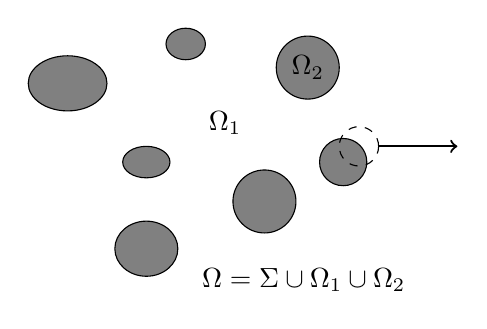
\begin{tikzpicture}
        \foreach \x/\y/\ra/\r in {
        1/3/0.2/0.25,
        2.55/2.7/0.4/0.4,
        0.5/0.4/0.35/0.4,
        2/1/0.4/0.4,
        3/1.5/0.3/0.3,
        0.5/1.5/0.2/0.3,
        -0.5/2.5/0.35/0.5}{
            \draw[fill=gray](\x,\y) ellipse(\r cm and \ra cm);
        }
        \draw[dashed](3.2,1.7)circle(0.25);
        % \draw[thick,->](3.2,1.7)++(0.1767,0.1767)--++(0.4,0.4)--++(1,0);
        \draw[thick,->](3.2,1.7)++(0.25,0)--++(1,0);
        \draw(2.55,2.7)node{$\Omega_2$};
        \draw(1.5,2)node{$\Omega_1$};
        \draw(2.5,0)node{$\Omega = \Sigma \cup \Omega_1 \cup \Omega_2$};
        % \draw(2.5,-1)node{$\Sigma = \sum_\alpha \Sigma_\alpha$};
        % \draw(2.5,-0.5)node{$\Omega_2 = \sum_\alpha \Omega_\alpha$};
    \end{tikzpicture}
    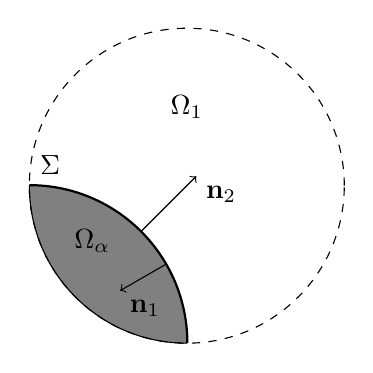
\begin{tikzpicture}%[scale = 0.9]
        \draw[very thick](0:2)arc(0:90:2)node[above right]{$\Sigma$};
        \draw[fill=gray](0:2)arc(0:90:2)arc(180:270:2);
        \draw[dashed](2,2)circle(2);
        \draw[->](1.42,1.42)--++(0.7,0.7)node[below right]{$\textbf{n}_2$};
        \draw[->](1.73,1)--++(-0.577,-0.333)node[below right]{$\textbf{n}_1$};
        \draw(2,3)node{$\Omega_1$};
        \draw(0.8,1.3)node{$\Omega_\alpha$};
    \end{tikzpicture}
    \caption{Scheme of the topology of dispersed two phase flows.}
    \label{fig:Scheme}
\end{figure}
From now on the $k$ indies will refer to either the phase $1$ or $2$, and we drop the time and position arguments in each functions. 
Then, the transport equation of $\chi_k$ can be written as \citep{drew1983mathematical,kataoka1986local,morel2015mathematical},
\begin{equation}
    \pddt \chi_k
    + \textbf{u}_I \cdot \nablabh \chi_k
    = 0,
    \label{eq:dt_chi_k}
\end{equation}
where $\textbf{u}_I$ is the velocity of $\Sigma(t)$.
Besides, it can be shown \citep{tryggvason2011direct,drew1983mathematical,kataoka1986local,bothe2022sharp} that,
\begin{equation}
    \nablabh \chi_k
    = - \delta_I \textbf{n}_k
    \label{eq:grad_chi_k}
\end{equation}
where we have introduced the Interface Indicator Function (IIF) defined as $\delta(\textbf{y}-\textbf{y}_I)$, with $\delta$ being the Dirac-delta function and $\textbf{y}_I$ the position vectors lying on the domain $\Sigma(t)$.
We also define $\textbf{n}_k$ as the outward normal vector of the domain $\Omega_k$.
Taking the gradient of \ref{eq:dt_chi_k} yields the IIF transport equation namely,
\begin{equation}
    \pddt \delta_I
    + \nablabh \cdot \left[(\textbf{u}_I\cdot\textbf{n})\textbf{n} \delta_I\right]
    = \delta_I (\textbf{u}_I\cdot\textbf{n})(\nablabh \cdot\textbf{n})
\end{equation}
As pointed out by \citet{morel2007surface}, it is more convenient to rewrite this equation under the following form,
\begin{equation}
    \pddt \delta_I
    + \nablabh \cdot (\delta_I \textbf{u}_I)
    = \delta_I \nablabhI \cdot \textbf{u}_I.
    \label{eq:dt_delta_I}
\end{equation}
where we introduced the surface divergence operator defined as $\nablabhI \cdot ()= (\textbf{I}-\textbf{nn})\cdot \nablabh \cdot ()$.
Likewise, we can derive an expression for the gradient of $\delta_I$ by taking the gradient of \ref{eq:grad_delta_I} yielding,
\begin{equation}
    % &
    \nablabh\delta_I 
    = \textbf{n} \cdot \nablabh (\textbf{n} \delta_I),
    % &
    % \pddt\delta_I 
    % = - \textbf{n} \cdot \nablabh (\textbf{u}_I  \cdot \textbf{n} \delta_I)
    \label{eq:grad_delta_I}
\end{equation}


Let $f_k(\textbf{y})$ being a volumetric property of the flow solely defined in $\Omega_k(t)$.
Likewise, let $f_I(\textbf{y})$ be an arbitrary surface property defined on $\Sigma(t)$.
Then it is possible to derive the local conservation equations for volumetric and surface quantities \citep{bothe2022sharp,morel2015mathematical,tignol1986modelisation}, using Reynolds transport theorem  and divergence theorem on an arbitrary control volume.
These conservation laws read as, 
\begin{align}
    \label{eq:dt_f_k}
    \pddt f_k
    &= \nablabh \cdot \left(
        \bm{\Phi}_k
        - f_k\textbf{u}_k
        \right)
    + \textbf{S}_k
    & \text{ in } \Omega_k,&\\
    \pddt f_I  
    &= 
    \nablabhI \cdot (\mathbf{\Phi}_{I||} - f_I \textbf{u}_I)
    + \textbf{S}_I
    - \Jump{
        f_k (\textbf{u}_I - \textbf{u}_k)
        + \mathbf{\Phi}_k
     } 
    & \text{ on } \Sigma&
    \label{eq:dt_f_I}
\end{align}
for respectively the volumetric and surface properties.
In \ref{eq:dt_f_I} we introduced the notation $\Jump{\ldots}$ to indicate the sum over both phases, i.e. $\sum_{k=1}^2 [\ldots] \cdot \textbf{n}_k$. 
Where we introduced $\bm{\Phi}_k$ and $\bm{\Phi}_I$ as the non-conservative flux tensor corresponding to $f_k$ and $f_I$. 
The non-conservative flux is often expressed through a constitutive equation depending on the nature of the flow such as the stress tensor for the momentum.
$\textbf{S}_k$ and $\textbf{S}_I$ is defined as the volumetric source term of respectively the phase $k$ and at the interface $\Sigma$.
It is important to notice that \ref{eq:dt_f_k} and \ref{eq:dt_f_I} are solely defined in respectively $\Omega_k$ and $\Sigma$, therefore these equations are referred as local conservation equations.

To generalize these equations over the domain $\Omega$ we follow the formalism of \citet{drew1983mathematical,marle1982macroscopic} and \citet{kataoka1986local} for the volumetric quantities.
Indeed, to any local quantities $f_k$ defined in $\Omega_k$, we assign the field $\chi_k f_k$ which is defined in $\Omega$. 
Similarly, for any local surface quantities $f_I$ defined on $\Sigma$ we assign the field quantity $\delta_I f_I$ defined on $\Omega$. 
Then, multiplying \ref{eq:dt_f_k} and \ref{eq:dt_f_I} by respectively $\chi_k$ and $\delta_I$, and making use of \ref{eq:dt_chi_k} and \ref{eq:dt_delta_I} gives, 
\begin{align}
    \pddt (\chi_k f_k)
    &= \nablabh \cdot (\chi_k \bm{\Phi}_k - \chi_k f_k \textbf{u}_k)
    + \chi_k \textbf{S}_k
    + \delta_I\left[
        \bm{\Phi}_k
        + f_k
        \left(
            \textbf{u}_I
            - \textbf{u}_k
        \right)
    \right]
    \cdot \textbf{n}_k ,
    % & \forall \textbf{y} \in \Omega&
    \label{eq:dt_chi_k_f_k}\\
    \pddt (\delta_If_I)  
    &= 
    \nablabh \cdot (\delta_I \mathbf{\Phi}_{I||} - \delta_I f_I \textbf{u}_I)
    +\delta_I\textbf{S}_I 
    - \delta_I \Jump{
    f_k (\textbf{u}_I - \textbf{u}_k)
    + \mathbf{\Phi}_k
    }.
    \label{eq:dt_delta_I_f_I}
\end{align}
We obtained $k$'s equations defined over the domain $\Omega$ for the bulk quantities, and third global equations for the surface quantities also valid over $\Omega$. 
The transformation of these equations from local to global conservation makes appear a term on the RHS of \ref{eq:dt_chi_k_f_k} representing the interfacial transfer of $f_k$ and $\mathbf{\Phi}_k$, while the surface transport equation did not change fundamentally. 
The set of equations formed by \ref{eq:dt_chi_k_f_k} for $k =1,2$ is commonly known as the \textit{two-fluid} formulation of multiphase flows, to which we add the \textit{jump condition} across the phase given by \ref{eq:dt_delta_I_f_I} \citep{morel2015mathematical,tryggvason2011direct,drew1983mathematical,kataoka1986local}. 
In this work, we prefer to think of those equations as a set of three equations, formed by \ref{eq:dt_chi_k_f_k} for the volumetric conservation equations and \ref{eq:dt_delta_I_f_I} for the surface conservation equations. 

Now that we properly defined the volumetric and surface conservation laws over $\Omega$, let's derive of two phase flows.
We now define any bulk quantity $f$ as $f = \sum_k \chi_k f_k + \delta_I f_I$.
Then adding \ref{eq:dt_chi_k_f_k} for $k=1,2$ and \ref{eq:dt_delta_I_f_I} give the commonly known as the \textit{single-fluid} formulation,
\begin{equation}
    \pddt f
    = \nablabh \cdot (\bm{\Phi} - f \textbf{u})
    + \textbf{S}.
    \label{eq:dt_f}
\end{equation}
Actually, it is more common in the literature to define the bulk quantities as $f = \sum_k \chi_k f_k$ and consider the interfacial terms as source terms as it is often neglected \citep{morel2015mathematical,tryggvason2011direct}. 
Nevertheless, in this work we consider a general case without approximation therefore it is more convenient to think of the bulk quantities as a sum of three phase quantities. 

\subsection{The averaged conservation equations}
\label{sec:avg_def}
In this study, we employ the ensemble average technique to establish the averaged conservation equations. 
This method is just one of several averaging approaches, including the volume average method \citep{jackson1997locally} and time averaging \citep{ishii2010thermo}. 
Despite their differences, all these techniques yield the same set of averaged equations \citep{jackson1997locally,zhang1997momentum}.
In the following we recall some properties of the ensemble average operator. 
Let, $P(\FF)$ be the probability density function that describes the probability of finding the flow in the configuration $\FF$. 
We note $d\PP = P(\FF) d\FF$ the probable number of flows located in the incremental region of the phase space $d\FF$ around the point $\FF$. 
It follows from this definition, that the ensemble average of an arbitrary local property $f^0(\textbf{x},t;\FF)$ defined on the whole space $\Omega$, is,
\begin{equation}
    f(\textbf{x},t)
    = \avg{f^0}(\textbf{x},t)
    =\int f^0(\textbf{x},t;\FF) d\mathscr{P}. 
    \label{eq:avg}
\end{equation}  
Note that we dropped the super script $^0$ on $f(\textbf{x},t)$ to indicate that this is an averaged quantity. 
The macroscopic variables are averaged over all $\FF$, and therefore depend only on $\textbf{x}$ and $t$.
Thus, we omit the arguments of the averaged fields, as this notation eliminates any potential ambiguity. 
The ensemble average quantities are assumed to satisfy the following properties \citep{drew1983mathematical}
\begin{align}
    \label{eq:avg_properties}
    \avg{f^0+h^0} &= f+h, \\ 
    \avg{\avg{f^0}h^0} &= fh, \\
    \avg{\pddt f^0} 
    &= \pddt f, \\ 
    \avg{\grad f^0}
    &= \grad f. 
\end{align}
were $f$ and $h$ are two arbitrary Eulerian fields. 
The first two relations are called the Reynolds' rules, the third one is the Leibniz' rule and the last one, is the Gauss' rule \citep{drew1983mathematical}.
Additionally, for any phase quantity defined in $\Omega_k$ we introduce the definition, 
\begin{equation}
    \phi_k f_k (\textbf{x},t) = \avg{\chi_k f_k^0},
    \label{eq:1_avg}
\end{equation}
where $\phi_k(\textbf{x},t) = \avg{\chi_k}$ is the volume fraction of the phase $k$.
And $f_k$ is the average of the field $f_k^0$ conditioned on the presence of the phase $k$ in the configuration $\FF$ at $\textbf{x}$ and time $t$.
Equally, for interface quantities we have 
\begin{equation}
    \phi_I f_I (\textbf{x},t) = \avg{\delta_I f_I^0},
\end{equation}
with $\phi_I = \avg{\delta_I}$ the interfacial area concentration function. 
Here, $f_I$ is the average of $f^0_I$ conditioned on the presence of an interface in the configuration $\FF$ at $\textbf{x}$ and time $t$. 
Additionally, we define the field of fluctuation of a given quantity around its mean as,
\begin{align}
    f'(\textbf{x},t,\FF) = f^0(\textbf{x},t,\FF) - f(\textbf{x},t).
    \label{eq:def_fluctu}
\end{align}
This relation applies to phase averaged quantities such that $f'_k = f^0_k - f_k$ and $f'_I = f^0_I - f_I$. 


Applying the ensemble average on \ref{eq:dt_chi_k_f_k} and \ref{eq:dt_delta_I_f_I} and considering the properties from \ref{eq:avg_properties} to \ref{eq:def_fluctu}, yields the general form of the averaged equations of multiphase flows, namely,
\begin{align}
    \pddt (\phi_k f_k)
    +\div (\phi_k f_k \textbf{u}_k - \mathbf{\Phi}_k^\text{eq})
    &= 
    \phi_k s_k
    + \avg{\delta_I\left[
        \mathbf{\Phi}_k^0
        + f_k^0
        \left(
            \textbf{u}_I^0
            - \textbf{u}_k^0
        \right)
    \right]
    \cdot \textbf{n}_k} ,
    \label{eq:avg_dt_chi_f}\\
    \pddt (\phi_I f_I)
    +\div (\phi_I f_I \textbf{u}_I- \mathbf{\Phi}_{I}^\text{eq})
    &= 
    \phi_I s_I
    - \avg{\delta_I 
    \Jump{
    f_k^0 (\textbf{u}_I^0 - \textbf{u}_k^0)
    + \mathbf{\Phi}_k^0
    } 
     },
    \label{eq:avg_dt_delta_f}
\end{align}
with, 
\begin{align*}
    \mathbf{\Phi}_k^\text{eq}
    = \avg{\chi_k f_k' \textbf{u}_k'}
    - \phi_k \bm\Phi_k,
    &&
    \mathbf{\Phi}_{I}^\text{eq}
    = \avg{\delta_I f_I' \textbf{u}_I'}
    - \phi_I \bm\Phi_I. 
\end{align*}
These equations are to be solved for the averaged field $\phi_k,\phi_I,f_k$ and $f_I$ with a complementary equation of volume conservation, i.e. $\phi_f+\phi_d+\phi_I = 1$.
The main differences between these equations and their microscale counterparts (\ref{eq:dt_f_k} and \ref{eq:dt_f_I}) are:
(1) The unknowns are now averaged quantities,
(2) Factors $\phi_k$ and $\phi_I$ are introduced in front of all the terms, and
(3) The additional terms $\avg{\chi_k f_k' \textbf{u}_k'}$ and $\avg{\delta_I f_I' \textbf{u}_I'}$ appear, representing the covariance between the conserved quantity ($f_k$ or $f_I$) and the local velocities.  
For a complete understanding, we derived the mass, momentum, and energy averaged equations in \ref{ap:two-fluid_model}. 
These are derived considering the simplifying hypothesis exposed in \ref{ap:hypothesis}. 
In addition, \ref{ap:two-fluid_model} presents how to derive the secondary averaged equations of the averaged energy $E_k$, i.e. the equation for the mean internal energy $e_k$, the pseudo turbulent energy $k_k = \frac{1}{2\phi_k}\avg{\chi_k (u'_k)^2}$, and the averaged kinetic energy $(u_k)^2/2$.  


It is important to highlight that the two-fluid model fails to adequately distinguish between the two phases, as evidenced by the \textit{symmetry} $k = 1$ and $2$ in the aforementioned equations. This symmetry does not hold physically because the dispersed phase possesses a distinct topological nature compared to the continuous phase. 
More importantly, in a dispersed two-phase flow system the closure terms are expressed as a function of the Lagrangian properties of the particles whereas this system of equation provides us with continuously averaged quantities. 
Specifically, the mean drag force or torque term in the averaged momentum equation is expressed as a function of the center of mass linear and angular velocity  of the particles. 
Whereas this system of equation provides us with the phase averaged velocity of the whole phase not with no consideration for the particles properties.  
Therefore, in the subsequent section, we will introduce a kinetic model specifically devoted to the dispersed phase. 
As illustrated below, the equations governing the dispersed phase are more comprehensive as they bear a resemblance to the equations governing a single particle.



\section{Lagrangian equations for the dispersed phase}
\label{sec:Lagrangian}

In this section, we present a Lagrangian-based model capable of describing the dispersed phase with an arbitrary order of accuracy.

\subsection{Fundamental properties}

At this stage, we define some fundamental properties associated to each particle labeled $\alpha$.
Following the strategy of \citet{lhuillier2009rheology,lhuillier1992volume,zaepffel2011modelisation} and \citet[Chapter 2]{morel2015mathematical}
we define the mass $m_\alpha$, position of center of mass $\mathbf{x}_\alpha$, and the momentum $\textbf{p}_\alpha$ of the particle $\alpha$, as
\begin{align}
    m_\alpha(t,\FF)
    = \intO{ \rho_d  }, 
    &&
    \textbf{x}_\alpha(t,\FF)
    = \frac{1}{m_\alpha(t,\FF) }\intO{ \rho_d \textbf{x} }, 
    &&\textbf{p}_\alpha(t,\FF) 
    = \intO{ \rho_d \textbf{u}_d^0 }.
    \label{eq:mass_pos}
    % \label{eq:momentum_energy}
\end{align}
$\Omega_\alpha(t,\FF)$ is the time-dependent domain occupied by the particle $\alpha$ (see \ref{fig:Scheme}). 
Subsequently, we define the velocity of the particle center of mass as
\begin{equation*}
\textbf{u}_\alpha = \frac{d \textbf{x}_\alpha}{dt}.
\end{equation*}
Replacing $\textbf{x}_\alpha$ by its definition (\ref{eq:mass_pos}) we obtain
\begin{equation*}
    \textbf{u}_\alpha = \frac{1}{m_\alpha}
    \frac{d}{dt} 
    \left(
        \intO{ \rho_d \textbf{x} }
    \right)
    - \frac{1}{m_\alpha^2} \frac{d}{dt} \left(\intO{ \rho_d } \right)
    \intO{ \rho_d \textbf{x} }.
\end{equation*}
%\tb{ A finaliser
Using the Reynolds transport theorem (\ref{eq:reynolds_transport}) for both terms in parentheses and making use of the conservation of mass (\ref{eq:dt_rho}) and the definition of $\textbf{x}_\alpha(t,\FF)$ in the last term, gives
\begin{equation}
    \textbf{u}_\alpha = 
    \frac{1}{m_\alpha}\intO{ \left[
        \pddt (\textbf{x}\rho_d ) + \div\left(\textbf{u}_d \textbf{x} \rho_d\right) 
    \right]} \\
    + \frac{1}{m_\alpha}\intS{ \textbf{x} \rho_d(\textbf{u}_I   - \textbf{u}_d) \cdot \textbf{n}_d }
    -  \frac{\textbf{x}_\alpha}{m_\alpha}    \intS{ \rho_d(\textbf{u}_I   - \textbf{u}_d) \cdot \textbf{n}_d }
\end{equation}
Then by considering the mass conservation for the first term and noticing that $\grad \textbf{x} = \bm\delta$, for the second term gives, 
\begin{equation}
    \textbf{u}_\alpha(t,\FF) = \frac{1}{m_\alpha(t,\FF)} \left(
        \textbf{p}_\alpha(t,\FF)
        +  \intS{\rho_d \textbf{r} (\textbf{u}_I^0 - \textbf{u}_d^0)\cdot \textbf{n}_d }
        \right),
        \label{eq:dt_y_alpha}
\end{equation}
where $\textbf{r}(\textbf{x},t) = \textbf{x} - \textbf{x}_\alpha(t)$. 
In \ref{eq:dt_y_alpha}, it can be observed that the first component of the velocity represents the linear momentum divided by the mass of the particle. 
This corresponds to the mass-averaged velocity over the volume of the particle.
The second term in \ref{eq:dt_y_alpha} arises from the contribution of anisotropic mass transfer across the surface of the particle. 
This mass transfer leads to the motion of the particle's center of mass, thereby contributing to the total velocity.
To illustrate this concept, let us consider a fixed drop with no momentum lying over a very hot plate.
In this scenario, we assume that the plate is sufficiently hot to induce evaporation, specifically on the bottom portion of the drop.
Hence, under the effect of an anisotropic evaporation flux one may expect the second term to be non-negligible.
Consequently, the center of mass of the drop has a non-zero velocity in the opposite direction of the plate, even though the momentum is assumed to be zero.
Note that \ref{eq:dt_y_alpha} generalized usual expression of the center of mass velocity whom neglect the second term.
In the following, for the sake of brevity we discard the dependency on $t$ and $\FF$ on the notations for all Lagrangian quantities denoted by the subscript $_\alpha$ and in particular $\Gamma_\alpha$ and $\Omega_\alpha$.
Nevertheless, the reader must understand that all Lagrangian quantities and integration domains subscribed by $_\alpha$ are time and configuration-dependent. 

The particle's internal relative motions or the \textit{inner velocity} is given by $\textbf{w}_d^0 = \textbf{u}_d^0 - \textbf{u}_\alpha$. 
Substituting the inner velocity in the momentum definition (\ref{eq:mass_pos}) yields
\begin{equation}
    \label{eq:momentum_definition_1}
    \textbf{p}_\alpha
    = m_\alpha \textbf{u}_\alpha
    + \int_{\Omega_\alpha} \rho_d \textbf{w}_d^0 d\Omega.
\end{equation}
Alternatively, from \eqref{eq:dt_y_alpha}, we obtain,
\begin{equation}
    \textbf{p}_\alpha
    =  m_\alpha \textbf{u}_\alpha
    - \int_{\Gamma_\alpha} \rho_d\textbf{r}(\textbf{u}_I^0 - \textbf{u}_d^0)\cdot \textbf{n}_d d\Sigma
    \label{eq:momentum_definition}
\end{equation}
Therefore, the momentum of a particle can be seen as a sum of the mean velocity plus the integral of the fluctuation (\ref{eq:momentum_definition_1}), with the latter being equivalent to minus the first moment of mass transfer term (\ref{eq:momentum_definition}).
Indeed, by identification we obtain : $\intO{ \rho_d \textbf{w}_d^0 } = - \intS{  \rho_d\textbf{r} (\textbf{u}_I^0 - \textbf{u}_d^0)\cdot \textbf{n}_d }$. 
Hence, the internal velocity fluctuations within a fluid particle do not contribute to the total linear momentum $\textbf{p}_\alpha$, as long as the anisotropic mass transfer is negligible.  
Only within this simplified context we can consider the classic relation $\textbf{p}_\alpha = m_\alpha \textbf{u}_\alpha$. 

\subsection{Conservation laws}

We assign to a particle indexed, $\alpha$, occupying the domain $\Omega_\alpha$ (see \ref{fig:Scheme}) an arbitrary Lagrangian property $q_\alpha$ defined by $q_\alpha  = \intO{ f_d^0}$.
Similarly, we define $q_{I\alpha} = \intS{ f_I^0}$ as an integrated surface property of the particle $\alpha$.

\subsubsection{Inside the volume}
To describe the evolution of any arbitrary Lagrangian quantity $q_\alpha$, we need to establish its time derivative.
Since $q_\alpha$ is an integral quantity with a time-dependent domain of integration, we apply the general Reynolds transport theorem for volume integral which gives for material domains (here the droplet volume),
\begin{equation}
    \ddt  \intO{f_d^0}
    = \intO{\left[ \pddt f_d^0 + \div\left(f_d^0\textbf{u}_d^0\right) \right]}\\
    + \intS{ f_d^0 (\textbf{u}_I^0-\textbf{u}_d^0)\cdot \textbf{n}_d }.
    \label{eq:reynolds_transport}
\end{equation}
By substituting the integrand of the first integral on the right-hand side (RHS) with \ref{eq:dt_f_k} we obtain the conservation law of the quantity $q_\alpha$, namely,  
\begin{equation}
    \ddt{q_\alpha}
    = \intO{ s_d^0 }
    + \intS{ \left[
        f_d^0 (\textbf{u}_I^0-\textbf{u}_d^0) 
        + \mathbf{\Phi}_d^0 
        \right] \cdot \textbf{n}_d }.
    \label{eq:dt_q_alpha}
\end{equation}
In \ref{eq:dt_q_alpha} we used the Gauss divergence theorem to show that
\begin{equation}
    \intO{\div \mathbf{\Phi}_d^0} = \intS{\mathbf{\Phi}_d^0 \cdot \textbf{n}_d}.
\end{equation}
The first term on the right-hand side of \ref{eq:dt_q_alpha} accounts for the total contribution of the source term $s_d^0$ to the particle $\alpha$,
while the second term is the surface integration of the exchange terms, which includes the phase transfer flux $f_d^0 (\textbf{u}_I^0-\textbf{u}_d^0)$ and the diffusive flux $\mathbf{\Phi}_d^0$. 


Let us consider the specific case of the momentum balance, i.e. $q_\alpha = \textbf{p}_\alpha$.
In this situation, \ref{eq:dt_q_alpha} reads
\begin{equation}
    \ddt  \textbf{p}_\alpha
    = \intO{ \rho_d\textbf{g} }
    + \intS{ 
        \left[
        f_d^0 (\textbf{u}_I^0-\textbf{u}_d^0)
         + \bm{\sigma}_d^0%\cdot\textbf{n}_d  
        %+ \mathbf{\Phi}_d^0 
        \right] 
        \cdot \textbf{n}_d },
\end{equation}
% first term reads as $\intO{ \rho_d\textbf{g} }$ 
The first term on the right-hand side represents the total weight acting on the particle $\alpha$, 
the second term represents the total source of momentum due to phase transfer, and it is expressed as, $\intS{ \rho_d \textbf{u}_d^0 (\textbf{u}_I^0-\textbf{u}_d^0)\cdot\textbf{n}_d }$,
and the last term $\intS{ \bm{\sigma}_d^0\cdot\textbf{n}_d }$, represents the resultant of the hydrodynamic forces acting on the surface of the particle.
It is important to notice that under this form, the exchange terms are expressed as integrals of dispersed phase fields denoted by the subscript $_d$.
Nevertheless, depending on the nature of the dispersed phase, these fields may not always be defined.
For rigid particles the stress within the particle $\bm{\sigma}_d^0$ is indeterminate \citep{guazzelli2011}.  
Hence, our objective is to express these exchange terms, in terms of the continuous phase field quantities instead of the dispersed phase fields, i.e. in terms of $\mathbf{\Phi}_f^0$ and $\textbf{u}_f^0$ rather than $\mathbf{\Phi}_d^0$ and $\textbf{u}_d^0$. 

\subsubsection{On the interfaces}
To address this issue in a general manner, let us derive the conservation equation for the integrated surface property $q_{I\alpha} = \intS{f_I^0}$.
To differentiate time-varying surface integrals within time, we make use of the general Leibniz rule, which states that for an arbitrary function $f_I^0$ defined on $\Gamma(t)$ we have the relation \citep{nadim1996concise}
\begin{equation}
    \ddt  \intS{f_I^0 }
    = \intS{ \left[
        \pddt f_I^0
        +   \gradI \cdot (\textbf{u}_I^0f_I^0)
    \right]}.
    \label{eq:surface_derivative}
\end{equation}
Substituting the right-hand side terms of \ref{eq:surface_derivative} with \ref{eq:dt_f_I}, gives,
\begin{equation}
    \ddt  q_{I\alpha}
    = \intS{ 
        s_I^0
    }
    - \intS{
 \Jump{
        f_k^0 (\textbf{u}_I^0 - \textbf{u}_k^0)
        + \mathbf{\Phi}_k^0
    }
    }.
    \label{eq:dt_q_I_alpha}
\end{equation}
We have used the surface divergence theorem applied to closed surfaces \citep{nadim1996concise}, it reads
\begin{equation}
    \intS{\gradI F}
    = 
    \intS{ F \textbf{n} (\div \textbf{n})},
    \label{eq:gauss_surface}
\end{equation} 
where $F$ is an arbitrary field.
This theorem demonstrates that any surface property parallel to the tangential plane of $\Gamma$, such as $\bm\Phi_{I||}$, satisfies the relation $\intS{\divI \bm\Phi_{I||}^0}
= 0$.
This explains why $\bm\Phi_{I||}$ does not appear in \ref{eq:dt_q_I_alpha}. 
\ref{eq:surface_derivative} can be interpreted as the conservation equation for the integrated surface property $f_I^0$, or as the jump condition of the $f^0_k$ integrated on the droplet surface. 
As discussed above we wish to get rid of $\mathbf{\Phi}_d^0$ in \ref{eq:dt_q_alpha}. 
To achieve this, we treat the particle's volume and surface as a unified entity and derive a conservation equation for $q_\alpha^\text{tot} = q_\alpha + q_{I\alpha}$. 
By summing \ref{eq:dt_q_alpha} and \ref{eq:dt_q_I_alpha} we directly obtain 
\begin{equation}
    \ddt  q_\alpha^\text{tot}
    = 
    \intO{ s_d^0 }
    + \intS{ s_I^0 }
    + \intS{ \left[
        f_f^0 (\textbf{u}_I^0-\textbf{u}_f^0) 
        + \mathbf{\Phi}_f^0 
        \right] \cdot \textbf{n}_d }. 
    \label{eq:dt_q_alpha_tot}
\end{equation}
This equation is the general form of the linear conservation law for the quantity $q_\alpha^\text{tot}$.
It applies to any particle immersed into a continuous phase following the local conservation, \ref{eq:dt_f_k} and \ref{eq:dt_f_I}.
We refer to this equation as the zeroth-order conservation equation or the linear conservation law for the particle $\alpha$.

We would like to highlight that due to the consideration of closed surface, the diffusive flux $\mathbf{\Phi}_{I||}^0$, plays no role at all in \ref{eq:dt_q_alpha_tot}.
Therefore, in the case of the linear momentum conservation law, the contribution of the momentum diffusive flux $\bm\sigma_{I||}^0$ exposed in \ref{eq:dt_rhoIu_I}, will not contribute to the momentum balance of a particle, and we obtain the relation 
\begin{equation}
    \ddt  \textbf{p}_\alpha^\text{tot}
    = 
    \intO{ \rho_d^0\textbf{g} }
    + \intS{ \rho_I^0\textbf{g} }
    + \intS{ 
        \left[
        f_d^0 (\textbf{u}_I^0-\textbf{u}_f^0)
        + \bm{\sigma}_f^0
        \right] 
        \cdot \textbf{n}_d }. 
\end{equation}
In this case, note that $\textbf{p}_\alpha^\text{tot} = \intO{\rho^0_d \textbf{u}_d^0}+\intS{\rho^0_I \textbf{u}_I^0}$ is the momentum of the particle's volume and surface. 
The latter might be negligible if the interface has a negligible weight. 
As a consequence, even in the presence of local Marangoni forces or surface viscous stresses (see \ref{eq:surface_fluxes}), the resultant of the surface diffusive fluxes would still cancel out in the linear momentum balance.
This fact has already been demonstrated by \citet{hesla1993note} who showed that the surface tension force does not contribute to the linear and angular momentum balance. 
Here, we have provided the general proof that the interfacial diffusive flux $\mathbf{\Phi}_{I||}^0$, which is present at the local scale according to \ref{eq:dt_f_I}, does not contribute to the zeroth-order conservation law of a particle with a closed surface.

For completeness, we exposed in \ref{ap:particles_eq} a clear derivation of the mass, momentum and total energy equations for a single particle.
The derivation takes place using the same hypothesis as it is exposed in \ref{ap:hypothesis}.
Especially, it is shown that the integration of the kinetic energy jump condition corresponds to the Lagrangian derivative of the particle surface, see \ref{eq:int_u_I2}. 

\subsection{Higher moment equations}

Because $f_d^0$ and $f_I^0$ are not always constant over the volumes and surfaces of the particles, it is interesting to introduce in the first place, the first moment of the quantities $f_d^0$ and $f_I^0$. 
They are defined as
\begin{align}
    &\textbf{Q}_\alpha 
    = \intO{ \textbf{r} f_d^0 },
    &\text{and}&
    &\textbf{Q}_{I\alpha}
    = \intS{ \textbf{r} f_I^0 },
    \label{eq:first_moment_definition}
\end{align}
where we recall that $\textbf{r} = \textbf{x} - \textbf{x}_\alpha$ is the distance between any point inside $\Omega_\alpha$ or $\Gamma_\alpha$, to the center of mass of the particle $\alpha$.
It is then possible to differentiate these moments with respect to time to obtain their conservation laws.
We use the Reynolds transport theorem (\ref{eq:reynolds_transport}) to describe the evolution of $\textbf{Q}_\alpha$ within time. 
It gives, 
\begin{equation*}
    \frac{d}{dt} \textbf{Q}_\alpha
      =  \intO{\left[
        \pddt(  f_d^0\textbf{r})
        + \div \left(  f_d^0 \textbf{r}\textbf{u}_d^0\right)
    \right]} 
    + \intS{  f_d^0 \textbf{r}  (\textbf{u}_I^0-\textbf{u}_d^0)\cdot \textbf{n}_d}
\end{equation*}
The first term on the right-hand side may be rewritten as
\begin{equation*}
\intO{ \left[
        \pddt(\textbf{r}  f_d^0)+ \div \left( \textbf{u}_d^0 \textbf{r} f^0_d\right) 
    \right]}
    = \intO{\textbf{r}\left[
        \pddt f_d^0
        + \div \left(f_d^0 \textbf{u}_d^0\right)
    \right] }
    + \intO{ f_d^0 \left[
        \pddt \textbf{r}
        +(\textbf{u}_d^0 \cdot \grad) \textbf{r}
    \right]}
\end{equation*}
Using \ref{eq:dt_f_k} for the first integral on the right-hand side, and considering the relation,
$  \pddt \textbf{r}
+ (\textbf{u}_d^0 \cdot \grad) \textbf{r}
= - \frac{d}{dt} \textbf{y}_\alpha  + \textbf{u}_d^0 
= \textbf{w}_d^0$,
for the second integral yields 
\begin{align}
    \frac{d}{dt} \textbf{Q}_\alpha
    % &= \intO{\textbf{r} \left[
    %      s_d^0  +  \div \bm\Phi_d^0
    % \right]}
    % +\intO{f_d^0  \textbf{w}_d }
    % + \int_{\Gamma_\alpha} \textbf{r}  f_d^0 (\textbf{u}_I^0-\textbf{u}_d^0)\cdot \textbf{n}_d  d\Sigma,\\
    = \intO{\left( 
        \textbf{r} s_d^0  
        + f_d^0  \textbf{w}_d 
        - \bm\Phi_d^0
    \right) }
    + \int_{\Gamma_\alpha} \textbf{r} \left[
        \bm\Phi_d^0
        + f_d^0 (\textbf{u}_I^0-\textbf{u}_d^0)
    \right]\cdot \textbf{n}_d  d\Sigma.
    \label{eq:dt_Q_alpha}
\end{align}
Where we have used the relation $\intO{\textbf{r}  \div \bm\Phi_d^0 }
= \intS{ \textbf{r} \bm\Phi_d^0 \cdot \textbf{n}_d }
- \intO{ \bm\Phi_d^0 }$. 
\ref{eq:dt_Q_alpha} is the first order moment conservation equation for the particle $\alpha$. 
Following the same procedure, and making use of \ref{eq:surface_derivative}, \ref{eq:gauss_surface} and \ref{eq:dt_f_I}, one can equally show that 
\begin{align}
    \ddt {\textbf{Q}_{I\alpha}}
    &= \intS{ \left(
        \textbf{r}s_I^0
        + f_I^0 \textbf{w}_I^0
        - \mathbf{\Phi}_{I||}^0
    \right) }
    - \intS{\textbf{r} 
    \Jump{\mathbf{\Phi}_k^0
        + f_k^0 (\textbf{u}_I^0 - \textbf{u}_k^0)
    }
    },
    \label{eq:dt_Q_I_alpha}
\end{align}
where $\textbf{w}_I^0 = \textbf{u}_{I||}^0 - \textbf{u}_\alpha$.
In \ref{eq:dt_Q_alpha}, we recognize the first moment of the source term $s_d^0$, the first moment of the diffusive flux term $\bm\Phi_d^0\cdot\textbf{n}_d$ and the first moment of phase exchange term, $f_d^0 (\textbf{u}_I^0-\textbf{u}_d^0)\cdot\textbf{n}_d$. 
Additionally, two supplementary terms appear in \ref{eq:dt_Q_alpha}, namely: the integral of the diffusive flux $\bm\Phi_d^0$, and a term related to the fluctuation of the internal velocity $f_d^0 \textbf{w}_d^0$.
Similar observations can be made for the first moment of surface equation \ref{eq:dt_Q_I_alpha}, as it shares similarities with \ref{eq:dt_Q_alpha}. 
In particular, it is worth noting the presence of the surface diffusive flux $\mathbf{\Phi}_{I||}^0$ in \ref{eq:dt_Q_I_alpha}.
This term will be further discussed in the following. 

For similar reason than the linear conservation equations, we sum \ref{eq:dt_Q_alpha} and \ref{eq:dt_Q_I_alpha} to expresses the conservation equation of the total first moment $\textbf{Q}_\alpha^\text{tot} = \textbf{Q}_\alpha + \textbf{Q}_{I\alpha}$, this yields 
\begin{multline}
    \ddt {\textbf{Q}_\alpha^\text{tot}}
    = \intO{ \left(
        \textbf{r} s_d^0         
        + f_d^0  \textbf{w}_d^0 
        - \mathbf{\Phi}_d^0
    \right) }
    + \intS{ \left(
        \textbf{r}s_I^0
        + f_I^0 \textbf{w}_I^0
        - \mathbf{\Phi}_{I||}^0
    \right) }
    + \intS{ \textbf{r} \left[
        \mathbf{\Phi}_f^0
        + f_f^0 (\textbf{u}_I^0-\textbf{u}_f^0)
    \right]\cdot \textbf{n}_d  }. 
    \label{eq:dt_Q_alpha_tot}
\end{multline}
Likewise, conservation laws can be derived for the $n^{th}$ order moments of volume and surface, i.e. for
\begin{align}
    \textbf{Q}_{\alpha n}
    = \intO{
         \underbrace{\textbf{rr}\ldots \textbf{rr}}_{n\text{ times}}
        f_d^0 },
        && \text{and} &&
    \textbf{Q}_{I\alpha n}
    = \intS{
         \underbrace{\textbf{rr}\ldots \textbf{rr}}_{n\text{ times}}
    f_I^0 },
    \label{eq:Q_n_definition}
\end{align} 
respectively. 
It can be shown that the derivative with time of $\textbf{Q}_{\alpha n}$ and $\textbf{Q}_{I\alpha n}$ do not involve any additional terms than in \ref{eq:dt_Q_alpha} and \ref{eq:dt_Q_I_alpha}, but rather just the $n^{th}$ order moments of the already presented terms.
We provide the full derivation of $\ddt{ \textbf{Q}_{\alpha n}}$ in \ref{ap:Moments_equations}.
In short, these higher order moments describe the distributions of the local quantities $f_d^0$ and $f_I^0$ inside the domain $\Omega_\alpha$ and $\Gamma_\alpha$, respectively.
Consequently, an infinite number of moments would be theoretically necessary to recover the fields $f_d^0$ and $f_I^0$ within $\Omega_\alpha$ and $\Gamma_\alpha$. 
Thus, one can reach an arbitrary order of accuracy upon the knowledge of an arbitrary number of moments for a given quantity.  

\subsection{Discussion}

To gain physical insight into the meaning of the first and higher moment equations, we now consider the case of mass and momentum conservation laws for a particle of arbitrary shape. 
For ease of understanding, we adopt the simplifying hypotheses presented in \ref{ap:hypothesis}. 
This implies that we consider no mass transfer across phases and no surface properties except for surface tension forces.

Following \ref{eq:Q_n_definition} we define the second-order moment of mass and the first-order moment of momentum as respectively,
\begin{equation}
    \textbf{M}_\alpha 
    = \intO{ \rho_d \textbf{r} \textbf{r} }
    \;\;\;\text{and}\;\;\;
    \textbf{P}_\alpha 
    = \intO{ \rho_d \textbf{r} \textbf{u}_d^0 }.
    \label{eq:first_moment_of_momentum_def}
\end{equation}
Note that $\textbf{M}_\alpha$ is analogous to the inertia tensor $\textbf{I}_\alpha$ in solid mechanics, both are related through the expression $\textbf{I}_\alpha = \bm\delta : \textbf{M}_\alpha - \textbf{M}_\alpha$.
For a constant density, the tensor $\textbf{M}_\alpha$ describes the second moment of the volume distribution around the particle center of mass.
Likewise, the tensor $\textbf{P}_\alpha$ describes the first moment of the velocity distribution within the particle volume. 
To provide a clearer physical interpretation of the moment of momentum tensor, we decompose $\textbf{P}_\alpha$ into two distinct parts. 
Namely, 
$\textbf{P}_\alpha = \textbf{S}_\alpha+\textbf{T}_\alpha$, where $\textbf{S}_\alpha$ represents the symmetric part and $\textbf{T}_\alpha$ is the antisymmetric part of $\textbf{P}_\alpha$.
Then, the tensors $\textbf{S}_\alpha$ and $\textbf{T}_\alpha$ correspond respectively to the stretching and angular momentum of the particle $\alpha$. 
The tensor $\textbf{S}_\alpha$ quantifies how fast and in which direction the particle gets elongated or flattened, in other words it represents the mean rate of deformation experienced by the particle.
The tensor $\textbf{T}_\alpha$ is related to the angular momentum of the particle denoted by the pseudo vector $\bm\mu_\alpha = \intO{ \rho_d \textbf{r} \times \textbf{u}_d^0 }$. 
Indeed, both  $\textbf{T}_\alpha$ and $\bm{\mu}_\alpha$ represent the angular momentum and are related through $(\bm{\mu}_\alpha)_i = \epsilon_{ijk} (\textbf{P}_\alpha)_{jk}= \epsilon_{ijk} (\textbf{T}_\alpha)_{jk}$, where $\bm\epsilon$ is the third order alternating unit tensor or Levi-Cita tensor. 
Lastly, we also introduce the scalar $M_\alpha =\frac{1}{3}\bm\delta : \textbf{P}_\alpha = \frac{1}{3}\intO{ \rho_d \textbf{r} \cdot \textbf{u}_d^0 }.$, which quantifies the rate at which the particle is being compressed or expanded.
To better explain the implication of these quantities on the particle kinematics we provide in \ref{eq:scheme}, three schemes representing possible inner velocity fields with their corresponding value of the moment of momentum tensor.
Note that in \ref{eq:scheme} we explicit
\begin{figure}[h!]
    \centering
    \hfill
    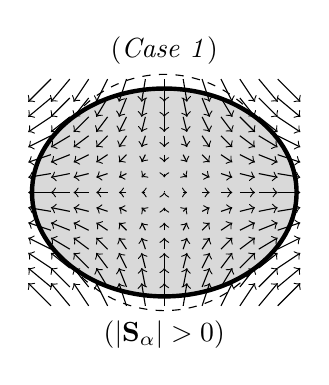
\begin{tikzpicture}[ultra thick,scale=0.6]
        \def\nRows{6}
        \def\nCols{6}
        \draw[dashed,thin] (0,0)circle(2.5);
        \draw[fill=gray!30] (0,0)ellipse(2.8 and 2.2);
        \foreach \x in {-\nRows,...,\nRows} {
            \foreach \y in {-\nCols,...,\nCols} {
                \pgfmathsetmacro\distance{veclen(\x*0.4, \y*0.4)};
                \pgfmathparse{\distance < 2.45 ? "blue" : "white"}
                \edef\colour{\pgfmathresult};
                \ifthenelse{\equal{\colour}{blue}}{                    
                    \draw[thin,->](\x*0.4,\y*0.4)--++(0.08*\x,-0.08*\y);
                }
            }
        }
        \node (txt) at (0,3){(\textit{Case 1})};
        \node (txt) at (0,-3){($|\textbf{S}_\alpha| > 0$)};
    \end{tikzpicture}
     \hfill
    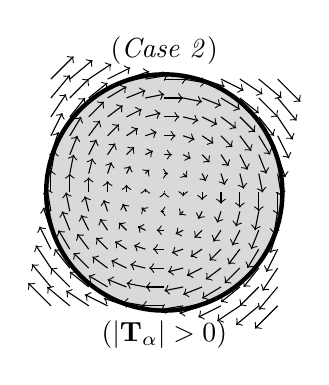
\begin{tikzpicture}[ultra thick,scale=0.6]
        \def\nRows{6}
        \def\nCols{6}
        \draw[fill=gray!30] (0,0)circle(2.5);
        \foreach \x in {-\nRows,...,\nRows} {
            \foreach \y in {-\nCols,...,\nCols} {
                \pgfmathsetmacro\distance{veclen(\x*0.4, \y*0.4)};
                \pgfmathparse{\distance < 2.5 ? "blue" : "white"}
                \edef\colour{\pgfmathresult};
                \ifthenelse{\equal{\colour}{blue}}{                    
                    \draw[thin,->](\x*0.4,\y*0.4)--++(0.08*\y,-0.08*\x);
                }
            }
        }
        \node (txt) at (0,3){(\textit{Case 2})};
        \node (txt) at (0,-3){($|\textbf{T}_\alpha| > 0$)};
    \end{tikzpicture}
    \hfill
    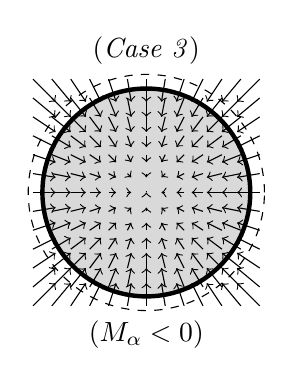
\begin{tikzpicture}[ultra thick,scale=0.6]
        \def\nRows{6}
        \def\nCols{6}
        \draw[dashed,thin] (0,0)circle(2.5);
        \draw[fill=gray!30] (0,0)circle(2.2);
        \foreach \x in {-\nRows,...,\nRows} {
            \foreach \y in {-\nCols,...,\nCols} {
                \pgfmathsetmacro\distance{veclen(\x*0.4, \y*0.4)};
                \pgfmathparse{\distance < 2.3 ? "blue" : "white"}
                \edef\colour{\pgfmathresult};
                \ifthenelse{\equal{\colour}{blue}}{                    
                    \draw[thin,->](\x*0.4,\y*0.4)--++(-0.08*\x,-0.08*\y);
                }
            }
        }
        \node (txt) at (0,3){(\textit{Case 3})};
        \node (txt) at (0,-3){($M_\alpha < 0$)};
    \end{tikzpicture}
    \hfill
    \caption{Graphical representation of the inner kinematics of an arbitrary particle under three scenarios. 
        The arrows represent the velocity field inside the particle, $\textbf{w}_d^0$, with the corresponding value of the moment of momentum tensor indicated below. 
        The operator $|\ldots|$ refers to the norm of the tensors. 
        According to the inner velocity field:
        (\textit{Case 1}) The particle experiences a mean rate of deformation, resulting in non-zero stretching of momentum along the principal axis of deformation;
        (\textit{Case 2}) The particle is rotating, leading to a non-zero angular momentum vector in the direction of rotation;
        (\textit{Case 3}) The particle undergoes compression, resulting in a negative trace of the moment of momentum.
    }
    \label{eq:scheme}
\end{figure}

Injecting, $f_d^0 = \rho_d$ in the second-order moment equation (derived in \ref{ap:Moments_equations}) we obtain :
\begin{equation}
    \ddt {\textbf{M}_\alpha}=2\textbf{S}_\alpha. 
    \label{eq:dt_M_alpha}
\end{equation}
which is the second-order moment of mass conservation equation. 
From \ref{eq:dt_M_alpha} we deduce that the evolution of the distribution of mass of a particle is solely motivated by the stretching of momentum $\textbf{S}_\alpha$. 
This implies that the angular momentum (not to be confused with the angular velocity) plays no role in the evolution of the second moment of mass. 
This is due to the symmetry of the tensor $\textbf{M}_\alpha$, which must be preserved after differentiation with respect to time.
Note that if the particle has a constant $\textbf{M}_\alpha$ under change of reference frame, such as for spherical particles where we can write $\textbf{M}_\alpha= \frac{a^2 m_\alpha}{5} \bm\delta$, then $\textbf{S}_\alpha=0$ since $\ddt \textbf{M}_\alpha = 0$ in this situation.
This argument has no restriction on the internal particle motions, thus it is also true for fluid particles with possible inner motion. 
Additionally, applying the trace operator on both sides of \ref{eq:dt_M_alpha}, yields the interesting relation $\ddt {M_\alpha}=\frac{2}{3}\bm\delta : \textbf{S}_\alpha$.
We can state that $M_\alpha = \lambda^\alpha_1(t)+\lambda^\alpha_d(t)+\lambda^\alpha_3(t)$, with $\lambda_i^\alpha$ for $i=1,2,3$, the eigenvalues of $\textbf{M}_\alpha$, as it is a symmetric tensor and thus always diagonalizable.
For undeformable particles, it is evident that the eigenvalues are not functions of time, implying $\ddt M_\alpha = 0$.  
Consequently, $\bm\delta : \textbf{S}_\alpha$ possesses the notable property of being zero whenever the particle shape remains constant, regardless of the orientation.

Now that we have described the kinematics of the particle shape, let us proceed to derive an equation for the dynamics of the particle shape, i.e. an equation for the moment of momentum. 
This equation is derived injecting $\textbf{Q}_\alpha = \textbf{P}_\alpha$ in \ref{eq:dt_Q_alpha_tot}, it reads, 
\begin{equation}
    \ddt {\textbf{P}_\alpha}
    - \intO{ \rho_d  \textbf{w}_d^0 \textbf{w}_d^0 }
    = 
    - \intO{\bm{\sigma}_d^0}
    - \intS{ 
        \gamma (\bm\delta - \textbf{nn})
    }
    + \intS{ \textbf{r}\bm{\sigma}_f^0\cdot \textbf{n}_d}.
    \label{eq:dt_P_alpha}
\end{equation}
On the left-hands side of \ref{eq:dt_P_alpha} we identify two inertial terms, i.e. the derivative of $\textbf{P}_\alpha$ and the internal velocity term $\intO{\rho_d\textbf{w}_d^0\textbf{w}_d^0 }$.
The inertia of the particle is then balanced by the terms on the right-hand side of the equation, namely: 
the integral of the particle internal stress $\intO{ \bm{\sigma}_d^0}$; 
the integral of the surface tension stress $\intS{ \gamma (\bm\delta- \textbf{nn}) }$; 
and the first moment of the hydrodynamic stress tensor, $\intS{\textbf{r}\bm\sigma_f^0\cdot \textbf{n}}$.
A discussion regarding the physical implications of this equation is provided below. 

The conservation equation of the angular momentum $\bm{\mu}_\alpha$ is obtained by taking the double contracted product of \ref{eq:dt_P_alpha} with $\bm\epsilon$, which gives 
\begin{equation}
    \ddt\bm{\mu}_\alpha
    =  
    % \textbf{t}_\alpha.
    \intS{ \textbf{r} \times \bm{\sigma}_f^0\cdot \textbf{n}_d }
    \label{eq:dt_mu_alpha}
\end{equation}
Notice that every term on the right-hand side of \ref{eq:dt_P_alpha} vanished due to their symmetric nature apart from the shew-symmetric part of the hydrodynamic stress, which is the hydrodynamic torque applied on the particle $\alpha$.
Particularly, the surface tension terms do not appear in the angular momentum balance since $\bm\sigma_I^0 = \gamma (\bm\delta-\textbf{nn})$ is symmetric, which is consistent with the findings of \citet{hesla1993note}. 
As a consequence, the surface tension does not affect the angular momentum regardless of the particle's shape. 
In the literature, it is common to include the torque due to inter-particular interactions in the angular momentum balance, as is done in \citet{jackson1997locally} and \citet{zhang1997momentum}.
In our case note that $\bm{\sigma}_f^0$ contains also short-range interaction forces which can be assimilated to the particle-particle interaction forces.

Taking the double contracted product of \ref{eq:dt_P_alpha} with the tensor $\bm\delta$ and using \ref{eq:dt_M_alpha}, yields directly  
% \begin{equation}
%     \frac{1}{2}\ddt^2 {M_\alpha}
%     - \frac{1}{3}\intO{ \rho_d \textbf{w}_d^0 \cdot \textbf{w}_d^0}
%     = 
%     \intO{p_d^0} 
%     % - \frac{1}{3}\intS{p_f^0 \textbf{r}\cdot \textbf{n}}
%     - \frac{2}{3} \gamma s_\alpha
%     - \frac{1}{3}\intS{p_f^0 \textbf{r}\cdot \textbf{n}}
%     + \frac{1}{3}\intS{\textbf{r}\cdot\bm\tau_f^0\cdot \textbf{n}},
%     \label{eq:dt_D_alpha}
% \end{equation}
\begin{equation}
    \frac{3}{2}\frac{d^2 M_\alpha}{dt^2}
    - \intO{ \rho_d \textbf{w}_d^0 \cdot \textbf{w}_d^0}
    = 
    - \intO{\bm\sigma_d^0:\bm\delta} 
    % - \frac{1}{3}\intS{p_f^0 \textbf{r}\cdot \textbf{n}}
    - \gamma 2 \intS{}
    % - \frac{1}{3}\intS{p_f^0 \textbf{r}\cdot \textbf{n}}
    + \intS{\textbf{r}\cdot\bm\sigma_f^0\cdot \textbf{n}}.
    \label{eq:dt_D_alpha}
\end{equation}
\ref{eq:dt_D_alpha}, corresponds to the isotropic work balance over the volume and surface of the particle. 
According to \ref{eq:dt_D_alpha}, the rate of compression of a particle, denoted by the second derivative of $M_\alpha$ evolves according to : 
the internal inertial term, $\intO{\rho_d \textbf{w}_d^0 \cdot \textbf{w}_d^0 }$;
the particle internal pressure $\intO{\bm\sigma_d^0:\bm\delta}$; 
the surface energy $\gamma\intS{  }$; 
and the trace of the hydrodynamic first moment $\intS{\textbf{r}\cdot\bm\sigma_f^0\cdot \textbf{n}}$.
If one considers spherical particles composed of compressible fluid, \ref{eq:dt_D_alpha} transforms into the Rayleigh-Lamb-Plesset equation. 
In the steady-state regime, this reduces to the Young-Laplace equation, as indicated by the presence of the first three terms on the right-hand side of \ref{eq:dt_D_alpha}. 

\tb{
    As an example we now consider the \textit{Rayleigh-Lamb-Plesset} equation for spherical bubbles with radius $a_\alpha(t)$. 
    As the droplets remain spherical while keeping a constant mass the moment of momentum and inner velocity field can be expressed, 
    \begin{align*}
        M_\alpha
        = \frac{m_\alpha}{5} a^2_\alpha(t),
        && 
        \textbf{w}_d^0
        = \frac{d a_\alpha}{dt}\frac{\textbf{r}}{a_\alpha(t)},
        \label{eq:expr1}
    \end{align*}
    where it is empathized that the radius $a_\alpha(t)$ is time-dependent. 
    The stress inside the bubbles might be expressed as compressible Newtonian fluids with no resistance to shear such that 
    \begin{equation}
        \bm\sigma_d^0 
        = 
        - p_d^0 \bm\delta
        - \lambda_d (\div \textbf{u}_d^0) \bm\delta
        % + \mu_d \left[\grad \textbf{u}_d^0 + (\grad \textbf{u}_d^0)^\dagger\right]
        = 
        - p_d^0 \bm\delta
        - \frac{3 \lambda_d}{a_\alpha} \frac{d a_\alpha}{dt}  \bm\delta
        % + \mu_d \left[\grad \textbf{u}_d^0 + (\grad \textbf{u}_d^0)^\dagger\right]
        \label{eq:StressBubbles}
    \end{equation}
    where $\lambda_d^0$ is the volume viscosity of the dispersed phase. 
    Assuming incompressible Newtonian fluid for the continuous phase and injecting the expressions \ref{eq:StressBubbles} and \ref{eq:expr1} into \ref{eq:dt_D_alpha} yields, 
    \begin{equation}
        \frac{1}{5} \rho_d^0 a_\alpha \frac{d^2 a_\alpha}{dt^2} 
        - 
        \frac{1}{a_\alpha} \frac{d a_\alpha}{dt} 
        \left(
            3 \lambda_d
            + 2 \mu_f 
        \right)
        = 
        +  \frac{1}{v_\alpha}\intO{p_d^0}
        -  \frac{1}{s_\alpha}\intS{p_f^0}
        - \gamma 2 \frac{3}{a}
    \end{equation}
    By expressing the fluid pressure on the surface in terms of the far field pressure (see daniel) one obtain the \textit{Rayleigh-Lamb-Plesset} equation. 
}

Taking the symmetric part of \ref{eq:dt_P_alpha}, and making use of \ref{eq:dt_M_alpha}, yields a dynamical balance equation for $\textbf{M}_\alpha$, namely
% \begin{multline}    
%     \frac{1}{2}\ddt^2{\textbf{M}_\alpha^\text{dev}}
%     - \intO{\left(
%         \rho_d\textbf{w}_d^0 \textbf{w}_d^0
%         - \rho_d\frac{1}{3}(\textbf{w}_d^0 \cdot \textbf{w}_d^0)\bm\delta\right)}
%     =  
%         - \mu_d \intO{\textbf{e}_d^0}
%         - \intS{\gamma\left(\frac{1}{3}\bm\delta-\textbf{nn}\right)}\\
%         + \frac{1}{2}\intS{\left(\textbf{r}\bm\sigma_f^0+ \bm\sigma_f^0\textbf{r} - \frac{2}{3}(\bm\sigma_f^0\cdot \textbf{r})\bm\delta\right)\cdot \textbf{n}}
%     \label{eq:dt_S_alpha}
% \end{multline}
\begin{equation}    
    \frac{1}{2}\frac{d^2 \textbf{M}_\alpha}{dt^2}
    - \intO{ \rho_d  \textbf{w}_d^0 \textbf{w}_d^0 }
    = 
    - \intO{\bm{\sigma}_d^0}
    - \intS{\gamma (\bm\delta - \textbf{nn})}
    + \intS{(\textbf{r}\bm{\sigma}_f^0+\bm{\sigma}_f^0 \textbf{r})\cdot \textbf{n}_d}.
    \label{eq:dt_S_alpha}
\end{equation}
On the left-hand side of \ref{eq:dt_S_alpha}, we recover the symmetric part of the inertial contributions. 
Especially, in opposition to \ref{eq:dt_P_alpha} we could substitute $\textbf{P}_\alpha+\textbf{P}_\alpha^\dagger$ by $\ddt \textbf{M}_\alpha$. 
Consequently, \ref{eq:dt_S_alpha} is a dynamical equation for the droplet mean deformation. 
In our case, only the external contribution $\frac{1}{2}\intS{\textbf{r}\bm\sigma_f^0\cdot \textbf{n}}$ is responsible for the generation of angular momentum, see \ref{eq:dt_mu_alpha}.
Taking the symmetric part of this tensor ultimately removes this contribution. 
Thus, on the right-hand side of \ref{eq:dt_S_alpha}, we identify the terms responsible for the droplet deformation exclusively.
Therefore, \ref{eq:dt_S_alpha} must be interpreted as an equation for the shape of the particle, represented by the tensor $\textbf{M}_\alpha$.

One might immediately recognize that this equation is in fact an extension of Batchelor’s famous result, 
\begin{equation}
    \intO{\bm{\sigma}_d^0}
    + \intS{\gamma(\bm\delta - \textbf{nn})}
    = \frac{1}{2}\intS{(\textbf{r}\bm\sigma_f^0+\bm\sigma_f^0\textbf{r})\cdot \textbf{n}},
    \label{eq:Batchelor}
\end{equation}
but with the consideration of the inertia of the particle.
\ref{eq:Batchelor} is particularly useful to express the unknown internal stress within solid particles (in which case $\gamma = 0$), in terms of surface integral, i.e. the stresslet $\intS{(\textbf{r}\bm\sigma_d^0+ \bm\sigma_d^0\textbf{r})\cdot \textbf{n}}$.
This relation is the main tool used to express the bulk stress of a suspension, it eventually leads to the computation of the famous Einstein equivalent viscosity, upon having a closed expression for the average of $\intS{(\textbf{r}\bm\sigma_d^0+ \bm\sigma_d^0\textbf{r})\cdot \textbf{n}}$ \citep{guazzelli2011}. 
In the inertial case, due to the limited degree of freedom of solid particles, the tensors $\textbf{M}_\alpha$ and the inner velocity field $\textbf{w}_d^0$ are fully determined by \ref{eq:dt_M_alpha} and \ref{eq:dt_mu_alpha}, indicating that $\textbf{M}_\alpha$ and $\textbf{w}_d^0$ can be utilized in \ref{eq:dt_S_alpha} not as unknowns but as source terms. 
Consequently, for solid particles, \ref{eq:dt_S_alpha} must be interpreted as a generalized equation for the undefined stress $\bm\sigma_d^0$ integrated on the volume of the particles.
Whether it is solid or fluid particles \ref{eq:dt_S_alpha} becomes particularly relevant for expressing the averaged stress within an inertial suspension in terms of Lagrangian properties, as discussed in section \ref{sec:averaged_eq}.

It is now clear that if the surface tension forces play no role in the linear and angular momentum equation, it does impact the moment of momentum $\textbf{P}_\alpha$ or more specifically its symmetric part $\textbf{S}_\alpha$.
Thus, the surface tension force impacts the hydrodynamic behavior of a particle solely through its action on $\textbf{S}_\alpha$, which is related to the shape of a particle represented by $\textbf{M}_\alpha$, through \ref{eq:dt_M_alpha}.
In \ref{ap:Moments_equations} we show how to derive the higher-order moment of momentum equations, which can also be viewed as formulas for the higher moments of the internal particle stress distribution. 
It is interesting to mention that in a recent study of \citet{dolata2021faxen} and \citet{zhou2020lamb} they use energy methods and recover the first two moments of momentum equations hidden into another but equivalent form, valid in the Stokes flow regime. 

Hence, the moment of momentum emerges as a quantity of utmost importance for all types of particles with variable shape or volume. In general, the first moments $\textbf{Q}_{\alpha}$ and $\textbf{Q}_{I\alpha}$ hold significant importance when considering particles with high internal gradients, i.e. when $\grad f_d^0$ or $\gradI f_I^0$ are non-negligible at the scale of one particle. 




\section{The hybrid model}
\label{sec:averaged_eq}
Two distinct descriptions can be applied to the dispersed phase, while only one description is applicable to the fluid phase. 
In this section, we derive averaged equations for the dispersed phase using Lagrangian conservation laws. 
Following this, we  discuss the equivalence between the particle or lagrangian averaged equations for the dispersed phase and the averaged equations for the dispersed phase presented in \ref{sec:two-fluid}.


%Two different descriptions are possible for the dispersed phase while one is available for the fluid phase. 
%In this part we first derive averaged equations for the dispersed phase based on Lagrangian conservation laws. 
%Then we provide a complete discussion regarding the equivalence between the "lagrangian" averaged equations for the dispersed phase and the averaged equations governing the dispersed phase presented in \ref{sec:two-fluid}. 
%based on 
%the set of equations just derived and the averaged equations governing the dispersed phase presented in \ref{sec:two-fluid}. 

\subsection{Dispersed phase averaged equations}

In the preceding section, we have described the dispersed phase using a Lagrangian framework. 
However, to ensure consistency with the Eulerian conservation equations that describe the continuous phase, it is necessary to extend the Lagrangian equations to an Eulerian description. 
The approach presented here follows the methodology pioneered by \citep{lhuillier1992ensemble}.
%In the last section, we have described the dispersed phase within a Lagrangian framework.
%However, to be consistent with the Eulerian conservation equations used to describe the continuous phase, we need to extend the Lagrangian equations to an Eulerian description. 
%The strategy exposed here follow the approach pionnered by \citep{lhuillier1992ensemble}.
%In order to achieve this,
We introduce the function $\delta_\alpha$, which is defined as follows, 
\begin{align}
    \delta_\alpha(\textbf{x},\textbf{x}_\alpha(t,\FF)) 
    = \delta(\textbf{x}-\textbf{x}_\alpha(t,\FF)),
    \label{eq:delta_alpha}
\end{align}
where $\delta$ is the Dirac function.
Note that we explicitly note the arguments $(t,\FF)$ to highlight that the position of the particle $\alpha$ is a function of time and of the flow configuration $\FF$.
Applying the chain rule yields \citep{lhuillier1998}%we may write the partial time derivative of $\delta_\alpha$ can be written as
%\begin{equation}
%\frac{\partial \delta_\alpha(\textbf{x},\textbf{x}_\alpha(t,\FF))}{\partial t} 
%=  \frac{\partial \textbf{x}_\alpha}{\partial t} 
%\cdot \frac{\partial \delta_\alpha}{\partial \textbf{x}_\alpha}(\textbf{x},\textbf{x}_\alpha(t,\FF)) .
%\end{equation}
%This leads to the following expression, 
\begin{equation}
    \pddt \delta_\alpha
    + \div (\textbf{u}_\alpha  \delta_\alpha)
    =0,
    \label{eq:dt_delta_alpha}
\end{equation}
where we used the identity, $\frac{\partial \delta_\alpha}{\partial \textbf{x}_\alpha}  = -\grad \delta_\alpha$ and the fact that $\textbf{u}_\alpha(t,\FF)$ is not a function of $\textbf{x}$. 
\ref{eq:dt_delta_alpha} does not apply in scenarios where topological changes occur, such as break-up or coalescence events. 
In these cases, a source term can be introduced on the right-hand side of \ref{eq:dt_delta_alpha}, similar to the approach used in population balance equations, to account for the birth or death of particles \citep{randolph2012theory}.
%It should be noted that \ref{eq:dt_delta_alpha} is not applicable if changes in topology, such as break-up or coalescence events, occur.
%In such cases it is possible, as it is done in population balance equations, to include a source term on the RHS of \ref{eq:dt_delta_alpha} to account for particle birth or death. 
%Multiplying each Lagrangian quantities $\text q_\alpha$ by $\delta_\alpha$ yields the field $\text q_\alpha(t,\FF)\delta_\alpha(\textbf{x},t,\FF)$, which is defined over the entire domain $\Omega$.
%Likewise, for any derivative of Lagrangian quantities, such as $\ddt \text q_\alpha$, we define its corresponding Eulerian field by multiplying $\ddt \text q_\alpha$ with $\delta_\alpha$ and show that :
By multiplying each Lagrangian quantity $\text q_\alpha$​ by $\delta_\alpha$​, we obtain the field $\text q_\alpha(t,\FF)\delta_\alpha(\textbf{x},t,\FF)$, which is defined throughout the entire domain $\Omega$. 
Similarly, for any derivative of a Lagrangian quantity, such as $\ddt \text q_\alpha$​, the corresponding Eulerian field is defined by multiplying $\ddt \text q_\alpha$ with $\delta_\alpha$ 
%This can be expressed as
Given that $\text q_\alpha(t,\FF)$ and $\textbf{u}_\alpha(t,\FF)$ do not depend on \textbf{x}, and by using Equation \ref{eq:dt_delta_alpha}, we obtain
\begin{equation}
    \delta_\alpha \ddt \text q_\alpha
    = \pddt (\delta_\alpha \text q_\alpha)
    + \div (\delta_\alpha \text q_\alpha \textbf{u}_\alpha).
    \label{eq:dt_delta_alpha_q_alpha}
\end{equation}
%where we have used the fact that $\text q_\alpha(t,\FF)$ and $\textbf{u}_\alpha(t,\FF)$ are not function of \textbf{x}, and we made use of \ref{eq:dt_delta_alpha}.
%Now let us consider a domain containing $N$ particles.
%We define what we call the \textit{particle field} of a quantity $\text q_\alpha$, as the sum of the $\delta_\alpha \text q_\alpha$ over all particles in the flow, namely $\displaystyle\sum_{\alpha=0}^N \delta_\alpha \text q_\alpha$.
%Notice that \ref{eq:dt_delta_alpha_q_alpha} remains valid for a sum of fields since derivative and sum operators commute.
Consider a domain containing $N$ particles. We define the \textit{particle field} for a quantity $\text q_\alpha$​ as the sum of $\delta_\alpha \text q_\alpha$ over all particles within the domain, expressed by $\displaystyle\sum_{\alpha=0}^N \delta_\alpha \text q_\alpha$​. 
Note that the formula given by \ref{eq:dt_delta_alpha_q_alpha} remains valid for the sum of such fields, since the operations of differentiation and summation commute.
%In the objective of obtaining averaged equations for the dispersed phase, we introduce the average of $\text q_\alpha$ as  
To obtain the averaged equations for the dispersed phase, we define the particle average of $\text q_\alpha$​ as
\begin{equation}
     n_p \text q_p(\textbf{x},t) = \avg{\sum_\alpha\delta_\alpha \text q_\alpha},
     \label{eq:p_avg}
\end{equation}
where, $n_p(\textbf{x},t) = \avg{\sum_\alpha \delta_\alpha}$ is the probability density of finding a particle center of mass in the infinitesimal volume $d\textbf{x}$ around \textbf{x}, and $\text q_p(\textbf{x},t)$ is the average of $\text q_\alpha$ conditionally on the presence of a particle at \textbf{x} and time $t$. 
To simplify the notations, we consider the shorthand \citep{lhuillier1998},
\begin{equation*}
    \sum_\alpha \delta_\alpha \to \delta_p, 
\end{equation*}
such that $\pavg{\text q_\alpha}=\avg{\sum_\alpha \delta_\alpha \text q_\alpha}=n_p\text q_p$.
Note that we used the subscript $_p$ on $\text q_p$ to denote that this represents a particle-averaged field, initially derived from Lagrangian quantities. 
%Furthermore, in view of equation   
Additionally, in light of \ref{eq:def_fluctu} we define the fluctuating part of a particle field $\text q_p$ as
\begin{equation}
    \text q_\alpha' = \text q_\alpha - \text q_p. 
    \label{eq:def_fluc_p}
\end{equation}

To obtain the particle phase averaged equations one multiply \ref{eq:dt_q_alpha_tot} and \ref{eq:dt_Q_alpha_tot} by $\delta_\alpha$ and apply the ensemble average (\ref{eq:avg}), this yields
\begin{align}
    \pddt (n_p\text Q_p)
    + \div (n_p \text Q_p \textbf{u}_p + \pavg{\textbf{u}_\alpha' \text Q_\alpha'})
    = \pOavg{ s_d^0 }
    + \pSavg{ s_I^0 }\nonumber\\
    + \pSavg{ \left[\mathbf{\Phi}_f^0 + f_f^0 (\textbf{u}_\Gamma^0-\textbf{u}_f^0) \right] \cdot \textbf{n}_d },
    \label{eq:avg_dt_dq_alpha_tot}\\
    \pddt (n_p\textbf{Q}_p^{(1)})
    + \div \left(n_p \textbf{Q}_p^{(1)} \textbf{u}_p + \pavg{\textbf{u}_\alpha' \textbf{Q}_\alpha^{(1)'}}\right)
    =\pOavg{ \left(
        \textbf{r} s_d^0         
        + f_d^0  \textbf{w}_d^0 
        - \mathbf{\Phi}_d^0
    \right) }\nonumber\\
    + \pSavg{ \left(
        \textbf{r}s_\Gamma^0
        + f_\Gamma^0 \textbf{w}_\Gamma^0
        - \mathbf{\Phi}_{\Gamma||}^0
    \right) }
    + \pSavg{ \textbf{r} \left[
        \mathbf{\Phi}_f^0
        + f_f^0 (\textbf{u}_\Gamma^0-\textbf{u}_f^0)
    \right]\cdot \textbf{n}_d  }.
    \label{eq:avg_dt_dQ_alpha_tot}
\end{align}
The derivation of the higher moment particle-averaged equations is provided in \ref{ap:Moments_equations}.
The only fluxes appearing in \ref{eq:avg_dt_dq_alpha_tot} and \ref{eq:avg_dt_dQ_alpha_tot} are the fluctuation tensors $\pavg{\textbf{u}_\alpha' \text q_\alpha'}$ and $\pavg{\textbf{u}_\alpha' \textbf{Q}_\alpha'}$. 
Therefore, the non-convective fluxes $\bm\Phi_d^0$ and $\bm\Phi_I^0$ do not play the role of macroscopic fluxes, as it is the case in \ref{eq:avg_dt_chi_f} and \ref{eq:avg_dt_delta_f}. Instead, they act as source terms in the first moment and higher moment equations. 
This distinction is the main structural differences between the Kinetic-like model (\ref{eq:avg_dt_dq_alpha_tot} and \ref{eq:avg_dt_dQ_alpha_tot}) and the two-phase flow model (\ref{eq:avg_dt_chi_f} and \ref{eq:avg_dt_delta_f}). 
In this study, \ref{eq:avg_dt_chi_f} and \ref{eq:avg_dt_delta_f} are referred to as the phase-averaged equations, while \ref{eq:avg_dt_dq_alpha_tot} and \ref{eq:avg_dt_dQ_alpha_tot} are called the particle-averaged equations. 


 





%\subsubsection*{Equivalence between particle and continuous models}
\subsection{Equivalence between particle-averaged and phase-averaged equations}
\label{sec:equivalence}
%To model the dispersed phase we can either use \ref{eq:avg_dt_chi_f} with $k=d$, or the particle-averaged equations: \ref{eq:avg_dt_dq_alpha_tot}, \ref{eq:avg_dt_dQ_alpha_tot} and possibly the higher moments equations in \ref{ap:Moments_equations}. 
%Consequently, it is fair to address the question of the compatibility and differences between both formalisms. 
To model the dispersed phase, there are two distinct approaches. 
We can either use \ref{eq:avg_dt_chi_f} with $k=d$, or we can employ the particle-averaged equations \ref{eq:avg_dt_dq_alpha_tot}, \ref{eq:avg_dt_dQ_alpha_tot} and potentially the higher moments equations found in \ref{ap:Moments_equations}.
Consequently, it is important to address the compatibility between these two formalisms.
It has been demonstrated in various studies \citep{buyevich1979flow,lhuillier1992ensemble,jackson1997locally,zhang1994averaged}, that phase-averaged quantities can be expressed as a Taylor series expansion of particle-averaged quantities. 

The aforementioned studies used the single-particle conditionally averaged approach to demonstrate this equivalence.  
In this work we use instead the ``distributional'' approach of \citet{pahtz2023general} since, as shown below it yields more general and simpler formulation. 
The dispersed phase indicator function $\chi_d$ can be expressed as a sum of phase indicator function, $\chi_d(\textbf{x},t,\FF) = \sum_\alpha\chi_\alpha(\textbf{x},t,\FF)$ where $\chi_\alpha =1$ in the particle domain $\Omega_\alpha(\FF,t)$ and $0$ otherwise. 
Thus, any dispersed phase quantity pertaining to a single particle can be written as, 
\begin{equation}
   f^0_d \chi_\alpha(\textbf{x},t,\FF)
   = 
   \int_{\mathbb{R}^3} 
    f^0_d \chi_\alpha(\textbf{x}_\alpha + \textbf{r},t,\FF)\delta(\textbf{x} - \textbf{x}_\alpha - \textbf{r}) 
    d\textbf{r} 
   \label{eq:taylor_f_d}
\end{equation}
Likewise, we assume that the interface indicator function $\delta_\Gamma$ can be partitioned into $N$ interface indicator function such that $\delta_\Gamma =  \sum_\alpha  \delta_{\Gamma\alpha}$.
In that case any surface-averaged quantities may be written, 
\begin{equation}
    f_\Gamma^0 \delta_\Gamma(\textbf{x},t,\FF) = 
    \sum_\alpha 
    \int_{\mathbb{R}^3} 
     f_\Gamma^0 \delta_{\Gamma\alpha}(\textbf{x}_\alpha + \textbf{r},t,\FF)\delta(\textbf{x} - \textbf{x}_\alpha - \textbf{r}) 
     d\textbf{r}. 
    \label{eq:taylor_f_I}
\end{equation}
% Notice that \ref{eq:taylor_f_d} and \ref{eq:taylor_f_I} are well-defined in the distributional sense since the integral on the right-hand side of both equations correspond to a convolution product.
Notice that the integral on the right-hand side of \ref{eq:taylor_f_d} and \ref{eq:taylor_f_I} correspond to a convolution product.
Additionally, since the Dirac distribution $\delta(\textbf{x} - \textbf{x}_\alpha - \textbf{r})$, is the unit of convolution \ref{eq:taylor_f_d} is verified (see \citet[Chapter 9]{appel2007}).
The convolution product of the Dirac delta and the derivative of the Heaviside distribution is also well-defined, see \citet[Chapter 9]{appel2007}.
It follows that \ref{eq:taylor_f_d} and \ref{eq:taylor_f_I} are well-defined in the distributional sense. 
Upon using the Taylor expansion of the Dirac delta function $\delta(\textbf{x} - \textbf{x}_\alpha - \textbf{r})$ in the neighborhood of $\textbf{r}=0$ one obtain,
\begin{equation}
\delta(\textbf{x} - \textbf{x}_\alpha - \textbf{r})
= \delta(\textbf{x} - \textbf{x}_\alpha)
- \textbf{r}\cdot\grad \delta(\textbf{x} - \textbf{x}_\alpha)
+ \frac{\textbf{rr}}{2}:\grad\grad\delta(\textbf{x} - \textbf{x}_\alpha) 
- \ldots.
% + \ldots
\label{eq:exp_delta}
\end{equation}
Injecting \ref{eq:exp_delta} into \ref{eq:taylor_f_d} and \ref{eq:taylor_f_I}, and noticing that the indicator functions, $\chi_\alpha$ and $\delta_\Gamma$, reduce the domain of integration from $\mathbb{R}^3$ to, $\Omega_\alpha$ and $\Gamma_\alpha$, respectively,  yields: 
\begin{align}
    f^0_d \chi_d
    =\delta_p\intO{f^0_d}
    - \div\left(\delta_p\intO{\textbf{r} f^0_d}\right)
    + \frac{1}{2}\grad\grad :\left(\delta_p\intO{\textbf{rr} f^0_d}\right)
    \ldots 
    \label{eq:fd_asympt}
   \\
   f_\Gamma^0 \delta_\Gamma 
   =\delta_p\intS{f^0_\Gamma}
   - \div\left(\delta_p\intS{\textbf{r} f^0_\Gamma}\right)
   + \frac{1}{2}\grad\grad :\left(\delta_p\intS{\textbf{rr} f^0_\Gamma}\right)
   \ldots 
   \label{eq:fG_asympt}
%    \\
\end{align} 
Where we recognize the zeroth, first and second order moments of $f_d^0$ and $f_\Gamma^0$, into \ref{eq:fd_asympt} and \ref{eq:fG_asympt}, respectively. 
Notice that even before applying any kind of averaging procedure \ref{eq:fd_asympt} and \ref{eq:fG_asympt} illustrates the connection between the dispersed phase fields, of the form $\chi_d(\ldots)$ or $\delta_\Gamma(\ldots)$, and the particle fields of the form $\delta_p(\ldots)$. 
It is interesting to notice that these relations hold in a distributional sense at a local level. 


Applying similar considerations to the interface indicator function $\delta_\Gamma$, and averaging over all configurations, we obtain the general relations that link continuous-averaged and particle-averaged fields, namely \citep{lhuillier1992ensemble,lhuillier1998,lhuillier2000bilan}, 
\begin{align}
    \avg{\chi_df_d^0} 
    &=  \pavg{\text q_\alpha}
        - \div  
        \pavg{\textbf{q}_\alpha^{(1)}}        
        + \frac{1}{2} \grad\grad : \pavg{\textbf{q}_{\alpha}^{(2)}}
        + \ldots  \label{eq:f_exp_chi} \\
    \avg{\delta_\Gamma  f_\Gamma ^0} 
    &=  \pavg{\text q_{\Gamma \alpha}}        
        - \div \pavg{\textbf{q}_{\Gamma\alpha}^{(1)}}
        + \frac{1}{2} \grad\grad : \pavg{\textbf{q}_{\Gamma\alpha}^{(2)}}
        + \ldots  
    \label{eq:f_exp_delta}
\end{align}
%\JL{j'ai ajoute la sommes des contributions dans les particules et de surfaces}
Summing \ref{eq:f_exp_chi} and \ref{eq:f_exp_delta} we obtain
\begin{equation}
    \avg{\chi_df_d^0+\delta_\Gamma  f_\Gamma ^0} = \pavg{\text Q_\alpha}
    - \div  
    \pavg{\textbf{Q}_\alpha^{(1)}}        
    + \frac{1}{2} \grad\grad : \pavg{\textbf{Q}_{\alpha}^{(2)}}
    + \ldots  \label{eq:f_exp}
\end{equation}
When considering an infinite number of terms in \ref{eq:f_exp} one might eventually obtain a converged approximation of $\avg{\chi_d f_d^0+\delta_\Gamma  f_\Gamma ^0}$. 
However, it is important to note that Taylor series have what is known as a \textit{radius of convergence} beyond which adding more terms does not necessarily improve the approximation \citep[Chapter 1]{appel2007}. 
In particular, for distances beyond a certain limit \textbf{r} the series might diverges depending on the behavior of the function $\avg{\chi_d f_d^0+\delta_\Gamma  f_\Gamma ^0}$ near the point $\textbf{x}$. 
For the purposes of this article, we will assume that the Taylor series has an infinite radius of convergence, although this assumption warrants further investigation.%function $f_d^0$ evaluated at a point $\textbf{x}_\alpha$ is greater than the particle size, then \ref{eq:f_exp} might converges and provides a good approximation.
%\JL{j'ai vraiment raccourci cette partie, car meme si je la trouve pertinente il y a des elements que je trouvais peu claire:
%\begin{itemize}
%\item tu dis que "to assume that $f_d$ is slowly variying at the scale of the particle", justement je ne pense pas que l'on veuille cela car sinon a quoi serve les moments d'ordres superieurs.
%Par ailleurs pr moi (mais peut etre que je me trompe), le rayon de convergence dsun' serie de Taylor n'a rien a voir avec le fait que la fonction dont on cherche la serie varie peu à l'endroit du developpement
%Enfin sur cette idée de precision de la série, pr moi le developpement en série se fait dans l'hypothèse ou la grandeur d'interet (moyennée) varie peut sur l'échelle des grandeurs macroscopiques
%en gros un developpement limite en $a/L$ ou $L$ est la taille des echelles macro.
%\end{itemize}
%}

%In brief, high care must be taken when using these kind of taylor expansion especially in that context since we do not know the exact form of $f_d$.  
%Nevertheless it is reasonable to assume that $f_d$ is slowly variying at the scale of the particle with a radius of convergence sufficiently large, in this case \ref{eq:f_exp} might provide a good approximation, 
%and we might expect an error of $\mathcal{O}[(a/L)^{n}]$ when the highest moment of the series is of order $n-1$ with $L$ being a macroscopic length scale. 
%It is within the context of this assumption that the following disscussion takes place. 

% \JL{pour l'instant j'ai eneleve la partie applicative (meme si elle me semble tres interessante). 
% D'ailleurs pq le second terme du dvt pr les conservation de la masse est nul ? 
% Ce serait bien de donner de petites lois d'echelles pr evaluer les ordres de grandeurs de chacun des termes.}
%Particularly we note that if $f_d^0 = \rho_d$ and $f_d^0 = \rho_d \textbf{u}_d^0$ we obtain, 
%\begin{align}
%    \label{eq:f_exp_exe1}
%    \phi_d \rho_d
%    = m_p n_p 
%    + \frac{1}{2}\grad^2 : (n_p\textbf{M}_p)+\ldots,\\
%    \phi_d \rho_d \textbf{u}_d
%    = m_p n_p \textbf{u}_p 
%    - \div (n_p\textbf{P}_p)+\ldots,
%    \label{eq:f_exp_exe}
%\end{align}
%respectively. 
%Meaning that $\phi_d\rho_d$ is related to the shape of the particles, represented by $\textbf{M}_p$ through \ref{eq:f_exp_exe1}.
%Additionally, considering \ref{eq:f_exp_exe}, it becomes apparent that the phase-averaged velocity $\textbf{u}_d$ encompasses the first moment of momentum $\textbf{P}_p$, which as discussed (in \ref{sec:Lagrangian}) accounts for the rotational, dilatational, and stretching motions of the particles. 
%The second terms on the right-hand side of \ref{eq:f_exp_exe1} and \ref{eq:f_exp_exe} become negligible for homogeneous mixture, i.e. if $n_p$, $\textbf{M}_p$ and $\textbf{P}_p$ are not function of \textbf{x}. 
%Conversely, these terms might become significant if $n_p$, $\textbf{M}_p$ or $\textbf{P}_p$ are space-dependent.
%For example, close to solid boundaries of a macroscopic flow strong gradients of $n_p$ are present at the particle length scale, since at the exact location of the boundaries we must respect $n_p = 0$. 
%In \cite{prosperetti1995finite} they study the importance of these terms, especially their remark that the approximation $\phi \approx n_p v_p$ may have significant consequence on the hyperbolicity of a two-phase flow system. 

To demonstrate the equivalence between the two formalisms, we follow a strategy similar to \citep{lhuillier2000bilan,lhuillier2009rheology}. 
%\JL{j'ai simplifie la description}
%We take the Taylor expansion of each terms in \ref{eq:avg_dt_chi_f} with $k=d$ using the relation \ref{eq:f_exp_chi}. 
%A similar procedure is followed for  the surface transport equations.
%Since we made use of the surface transport equations in the particles phase equations : \ref{eq:avg_dt_dq_alpha_tot} and \ref{eq:avg_dt_dQ_alpha_tot}, we also consider \ref{eq:avg_dt_delta_f} to prove equivalence. 
%As the resulting expression can become quite cumbersome, we will adopt the following definition. 
Let $\mathcal{C}_d$ denote the phase-averaged equation of conservation (\ref{eq:avg_dt_chi_f} with $k=d$) and $\mathcal{C}_\Gamma $ the averaged surface transport equation (\ref{eq:avg_dt_delta_f}).
Specifically, they are defined as follows
\begin{align}
    \mathcal{C}_d
    &=
    - \pddt \avg{\chi_df_d^0}
    - \div \avg{\chi_d \mathbf{\Phi}_d^0 - \chi_df_d^0 \textbf{u}_d^0}
    + \avg{\chi_d s_d^0}
    + \avg{\delta_\Gamma \left[
        \mathbf{\Phi}_d^0
        + f_d^0
        \left(
            \textbf{u}_\Gamma ^0
            - \textbf{u}_d^0
        \right)
    \right]
    \cdot \textbf{n}_d},\\
    \mathcal{C}_\Gamma 
    &= 
    -\pddt \avg{\delta_\Gamma f_\Gamma ^0}
    -\div \avg{\delta_\Gamma  f_\Gamma ^0 \textbf{u}_\Gamma ^0-\delta_\Gamma  \mathbf{\Phi}_{I||}^0 }
    + \avg{\delta_\Gamma s_\Gamma ^0} 
    - \avg{\delta_\Gamma  \Jump{
     \mathbf{\Phi}_k^0+
    f_k^0 (\textbf{u}_\Gamma ^0 - \textbf{u}_k^0)
    } }. 
\end{align}
It should be noted from \ref{eq:avg_dt_chi_f} and \ref{eq:avg_dt_delta_f} that $\mathcal{C}_d\equiv 0$ and $\mathcal{C}_\Gamma  \equiv 0$.
By applying the Taylor expansion to each term of $\mathcal{C}_d+\mathcal{C}_\Gamma $ as described in \ref{eq:f_exp} yields
\begin{equation}
    \mathcal{C}_d 
    + \mathcal{C}_\Gamma  
    = \mathcal{M}^{(0)} - \div \mathcal{M}^{(1)} + \frac{1}{2} \grad\grad : \mathcal{M}^{(2)} \ldots = 0,
    \label{eq:scheme_equivalence}
\end{equation} 
where the expressions for $\mathcal{M}^{(0)}$ and $\mathcal{M}^{(1)}$ are given by 
\begin{align}
    &\mathcal{M}^{(0)}
    = 
    - \avg{\delta_p \ddt {\text Q_\alpha}}
    % -\avg{\delta_p\textbf{u}_\alpha q_\alpha^\text{tot}}
    + \pOavg{ s_d^0 }
    + \pSavg{ s_\Gamma ^0 }
    + \pSavg{ 
    \left[\mathbf{\Phi}_f^0 
    + f_f^0 (\textbf{u}_\Gamma ^0-\textbf{u}_f^0) \right] \cdot \textbf{n}_d },\\
    &\mathcal{M}^{(1)} =
    -  \avg{\delta_p \ddt {\textbf{Q}_\alpha^{(1)}}}
    % - \avg{\delta_p\textbf{u}_\alpha \textbf{Q}_\alpha^\text{tot}}
     + \pOavg{ \left(
        \textbf{r} s_d^0         
        + f_d^0  \textbf{w}_d^0 
        - \mathbf{\Phi}_d^0
    \right) }
    + \pSavg{ \left(
        \textbf{r}s_\Gamma ^0
        + f_\Gamma ^0 \textbf{w}_\Gamma ^0
        - \mathbf{\Phi}_{\Gamma||}^0
    \right) } \nonumber\\
    &+ \pSavg{ \textbf{r} \left[
        \mathbf{\Phi}_f^0
        + f_f^0 (\textbf{u}_\Gamma ^0-\textbf{u}_f^0)
    \right]\cdot \textbf{n}_d  }.
\end{align}
Using \ref{eq:scheme_equivalence}, we reach one of the main conclusion of this study. 
We observe that $\mathcal{M}^{(0)}$ and $\mathcal{M}^{(1)}$ correspond to the zeroth and first-order moment equations, respectively. 
Additionally, as demonstrated in \ref{ap:Moments_equations} the coefficient $\mathcal{M}^{(n)}$ in \ref{eq:scheme_equivalence} represents the $n^{th}$ order moment in the particle-averaged conservation equation. 
From \ref{eq:scheme_equivalence} we conclude that combining \ref{eq:avg_dt_chi_f} for $k=d$ and \ref{eq:avg_dt_delta_f} effectively captures the particle moment equations through a Taylor expansion around the particle center of mass. 
%Thus, it is evident that one can use an arbitrary order of particles moments equations to achieve an arbitrarily accurate description of the dispersed phase, regardless of the properties of the multiphase flow.
Therefore, it is clear that by considering an arbitrary order of particle moments equations, one can achieve a highly accurate description of the dispersed phase.


The particle-averaged equations ($\mathcal{M}^{(0)}$\ldots $\mathcal{M}^{(n)}$) form a system with $n$ equations, one for each moment. 
In contrast, the dispersed phase-averaged equations ($\mathcal{C}_d$ and $\mathcal{C}_\Gamma$) consist of only two equations, which aggregate all the particle-averaged equations. 
This indicates that the particle-averaged formalism provides more information since it yields a separate equation for each moment, as opposed to the phase-averaged equations, which are limited to just two. 
This enhanced level of detail is achieved by considering the topology of the dispersed phase as demonstrated in the previous sections.
%Therefore, the particle-averaged formalism encompasses more information since it provides one equation for each moment, in opposition to the phase averaged equations which are only two. 
%Note that this gain in information has been possible through the consideration of the topology of the dispersed phase. 




%In \ref{ap:Moments_equations} we provide the expression for each $\mathcal{M}_n$ as well as the complete derivation of \ref{eq:scheme_equivalence}. 

%Another approach is to notice that $\mathcal{M}_n=0$ for all $n$ since \ref{eq:dt_Q_n} holds for all $n$. 
%Thus, we can rewrite \ref{eq:scheme_equivalence} such that all moments equations vanish, except $\mathcal{M}_0$ (which is arbitrary), this gives, 
%\begin{equation}
%    \mathcal{C}_d 
%    + \mathcal{C}_\Gamma 
%    = \mathcal{M}^{(0)} = 0.
%    \label{eq:proof2}
%\end{equation}
%This implies that equation \ref{eq:avg_dt_chi_f} with the surface transport equation \ref{eq:avg_dt_delta_f} is rigorously equivalent to \ref{eq:avg_dt_dq_alpha_tot}.
%\citet[Appendix A]{zhang1997momentum} provided evidences that the particle-averaged momentum equation is as legitimate as the phase-averaged momentum equation, which is consistent with \ref{eq:proof2}. 
%Additionally, \citet[Appendix A]{nott2011suspension} derived a similar expression than \ref{eq:proof2}, also in the case of the averaged momentum equation for suspension of solid spherical particles.
%Thus, in light of \ref{eq:proof2}, we generalize the conclusion of these authors and demonstrated that this is also true for all conservation laws regardless of the dispersed phase nature.  
%Considering the Lagrangian equations derived in \ref{sec:Lagrangian} this conclusion is not surprising at all since the phase-averaged and particle-averaged equations are all built on \ref{eq:dt_f_k} and \ref{eq:dt_f_I}.
%However, if one does not consider a proper derivation of the lagrangian balance equations as it is done in \ref{sec:Lagrangian} it might not be as obvious, even if \ref{eq:proof2} should remain true as demonstrated by \citet{zhang1997momentum,nott2011suspension}.
%Nevertheless, it is important to note that the conclusion given by \ref{eq:proof2} is not entirely objective since following the same procedure we could show equally that $\mathcal{C}_d+\mathcal{C}_\Gamma  = -\div\mathcal{M}^{(1)}=0$ and $\mathcal{C}_d+\mathcal{C}_\Gamma  = \frac{1}{2}\grad\grad:\mathcal{M}^{(2)}=0$ and so on. 
%Thus, it is more appropriate to examine the problem from the perspective of \ref{eq:scheme_equivalence}. 
%Namely, the particle-averaged equations ($\mathcal{M}^{(1)}$\ldots $\mathcal{M}^{(n)}$) constitute a system of equations with $n$ equations, one equation for each moment, while the phase-averaged equations ($\mathcal{C}_d$ and $\mathcal{C}_\Gamma$) is a system of two equations made of all the particle-averaged equations.
%Therefore, the particle-averaged formalism encompasses more information since it provides one equation for each moment, in opposition to the phase averaged equations which are only two. 
%Note that this gain in information has been possible through the consideration of the topology of the dispersed phase. 




\subsection{Conservation equations}

Given that the aim of this work is not only to demonstrate the equivalence but also to establish a comprehensive framework for analyzing dispersed two-phase flows, we now present \textit{the hybrid} set of conservation equations.
%Let us assume that we are interested by a macroscopic quantity $f$ that follows \ref{dt_f} at the local scale, (here $f^0$ could be the mass, momentum, concentration of chemical species etc \ldots) . 
The system of equations governing a macroscopic quantity $f$ consists of one equation for the fluid phase, which ensures the conservation of $f_f$ and $n$ equations for the dispersed phase, representing the conservation of the quantities $\textbf{Q}_p^{(n)}$.  
In its most general form, the hybrid description of $f$ can be expressed as
%The system of equations for a macroscopic quantity $f$ is constituted from one equation describing the fluid phase, meaning the conservation of $f_f$ and $n$ equations describing the dispersed phase, i.e. the conservation of the $\textbf{Q}_p^{(n)}$.  
%In all its generality the hybrid description of $f$ may be written,
\begin{align}
    \pddt (\phi_f f_f)
    +\div (\phi_f f_f \textbf{u}_f + \mathbf{\Phi}_f^\text{eff})
    &= 
    \phi_f s_f
    - \pSavg{\left[
        \mathbf{\Phi}_f^0
        + f_f^0
        \left(
            \textbf{u}_\Gamma^0
            - \textbf{u}_f^0
        \right)
    \right]
    \cdot \textbf{n}_d} ,
    \label{eq:avg_hybrid_dt_chi_f}\\
        % \pddt \pavg{[\textbf{Q}_\alpha^{(n)}]_{i_1\ldots i_n}^\alpha}
        % + \div  \pavg{\textbf{u}_\alpha [\textbf{Q}_\alpha^{(n)}]_{i_1\ldots i_n}^\alpha}
        % = \sum_{e=1}^{n} 
        % \pOavg{
        %     \prod^{n}_{\substack{ m=1 \\m \neq e}} r_{i_m} [f_d^0\textbf{w}_d^0  - \bm\Phi_d^0]_{i_e}
        % }\nonumber\\
        % + \pOavg{ \pri{1}{n} (\textbf{s}_d^0)_k }
        % +     
        % \sum_{e=1}^{n} 
        % \pSavg{
        %     \prod^{n}_{\substack{ m=1 \\m \neq e}} r_{i_m} [f_\Gamma^0\textbf{w}_\Gamma^0 - \bm\Phi_{||\Gamma}^0]_{i_e}
        % }
        % + \pSavg{ \pri{1}{n} (\textbf{s}_\Gamma^0)_k }\nonumber\\
        % +\pSavg{ \pri{1}{n} ([\bm\Phi_f^0 + \textbf{f}_f^0 \left(\textbf{u}_\Gamma^0 - \textbf{u}_f^0\right)]\cdot \textbf{n}_d)_k }.
        \pddt (n_p\text Q_p)
        + \div (n_p \text Q_p \textbf{u}_p + \pavg{\textbf{u}_\alpha' \text Q_\alpha'})
        &= \pOavg{ s_d^0 }
        + \pSavg{ s_\Gamma^0 }\nonumber\\
        &+ \pSavg{ \left[\mathbf{\Phi}_f^0 + f_f^0 (\textbf{u}_\Gamma^0-\textbf{u}_f^0) \right] \cdot \textbf{n}_d },
        \label{eq:avg_hybrid_q}
        \\
        \pddt (n_p\textbf{Q}_p^{(1)})
        + \div (n_p \textbf{Q}_p^{(1)} \textbf{u}_p + \pavg{\textbf{u}_\alpha' (Q_\alpha^{(1)})'})
        &=\pOavg{ \left(
            \textbf{r} s_d^0         
            + f_d^0  \textbf{w}_d^0 
            - \mathbf{\Phi}_d^0
        \right) }\nonumber\\
        + \pSavg{ \left(
            \textbf{r}s_\Gamma^0
            + f_\Gamma^0 \textbf{w}_\Gamma^0
            - \mathbf{\Phi}_{I||}^0
        \right) }
        &+ \pSavg{ \textbf{r} \left[
            \mathbf{\Phi}_f^0
            + f_f^0 (\textbf{u}_\Gamma^0-\textbf{u}_f^0)
        \right]\cdot \textbf{n}_d  },
        \label{eq:avg_hybrid_q_1}
        \\\nonumber
        \vdots
\end{align}
where the effective continuous phase non-convective flux term reads 
\begin{align}
    \mathbf{\Phi}_f^\text{eff}
    = \avg{\chi_f f_f' \textbf{u}_f'}
    - \avg{\chi_f \bm\Phi_f^0}
    - \pSavg{\textbf{r}\left[
        \mathbf{\Phi}_f^0
        + f_f^0
        \left(
            \textbf{u}_\Gamma^0
            - \textbf{u}_f^0
        \right)
    \right]
    \cdot \textbf{n}_d}
    + \div[\ldots].
\end{align}
%and \eqref{eq:avg_hybrid_dt_chi_f} is that in
The only difference in the conservation equation for the continuous phase between \eqref{eq:avg_dt_chi_f} and \eqref{eq:avg_hybrid_dt_chi_f} is the expansion of the exchange term $\avg{\delta_\Gamma \left[
    \mathbf{\Phi}_f^0
    + f_f^0
    \left(
        \textbf{u}_\Gamma ^0
        - \textbf{u}_f^0
    \right)
\right]
\cdot \textbf{n}_d}$ into a Taylor series in a similar way to \ref{eq:f_exp_delta}. 
The presence of the terms $\div[\ldots]$ in the expression for  $\mathbf{\Phi}_f^\text{eff}$ suggests that higher-order moments of the interphase exchange term are involved.
Similarly, the ellipsis below \ref{eq:avg_hybrid_q_1} implies that an arbitrary number of dispersed phase moment equations can be introduced. In this format, it becomes evident that the exchange term on the right-hand side of \ref{eq:avg_hybrid_dt_chi_f} is identical to that on the right-hand side of \ref{eq:avg_hybrid_q}. 
Additionally, in the effective flux $\mathbf{\Phi}_f^\text{eff}$ the exchange term from  \ref{eq:avg_hybrid_q_1} appears, and this property continues for higher-order moments.  
Consequently, the zeroth order exchange term in the equation for $\text Q_\alpha^{(0)}$ plays the role of a source term for $f_f$, while the first and higher order exchange terms act as a source into the higher moment equations, and contribute to the effective non-convective fluxes for $f_f$. 



The system of equations presented here offers a clear understanding of the roles of the dispersed phase non-convective flux terms, $\bm\Phi_d$ and $\bm\Phi_\Gamma$, in the particle phase conservation equation. 
As evidenced in \ref{eq:avg_hybrid_q}, $\bm{\Phi}_d$ and $\bm{\Phi}_\Gamma$  do not influence the lowest order particle-phase averaged conservation equation, i.e. the equation of $n_p \text Q_p$. 
However, \ref{eq:avg_dt_chi_f} (for $k = d$) and \ref{eq:avg_dt_delta_f}, show that the phase-averaged quantities $f_d$ and $f_\Gamma$, are affected by the non-convective fluxes at the particle surface and internally, since $\bm{\Phi}_d$ and $\bm{\Phi}_\Gamma$ appear in these equations.
This may seem contradictory at first, but it is important to note that $\bm{\Phi}_d^0$ and $\bm{\Phi}_\Gamma^0$ serve as source terms in the conservation equations for higher moments such as $\textbf{Q}^{(1)}_p$ \ldots $\textbf{Q}^{(n)}_p$, which are related to $f_d$ and $f_\Gamma$ through \ref{eq:f_exp}.
In summary, the non-convective fluxes $\bm{\Phi}_d$ and $\bm{\Phi}_\Gamma$  are not explicitly related to $\text Q_p$, regardless of particle nature or volume fraction. 
Instead, their influence on $\text Q_p$ is mediated through the closure terms in equation \ref{eq:avg_hybrid_q}, which may depend on the higher moments $\textbf{Q}^{(1)}_p$ \ldots $\textbf{Q}^{(n)}_p$ or other higher-order particle-related moments.%\footnote{This is typically the configuration observed in dilute flows of axisymmetric fibers within the Stokes regime. In this regime, the force acting on the fiber (which represents the exchange term in the momentum equation) is dependent on the orientation tensor, which in turn is directly linked to the second-order moment of the mass distribution.}. 
These moments, in turn, explicitly depend on $\bm{\Phi}_d$ and $\bm{\Phi}_\Gamma$ as indicated by \ref{eq:avg_hybrid_q_1}. 
%Consequently, it must be understood that the kinetic-like equations (\ref{eq:avg_dt_dq_alpha_tot}) is formally exact and apply for any type of particle and particle volume fraction, as long as the closure terms are well modeled and that the Taylor expansion used in these expressions reaches a convergence on the scale of the particles as discussed below.
%The reader is invited to interpret this expression for the specific case of the momentum conservation law. 







Now that we reached a clear understanding of the mathematical structures of the averaged two phase flow equation we start to expose the averaged set of equations which constitute the \textit{Hybrid model}. 
As, mentioned in \ref{sec:two-fluid} we consider the mass, momentum and energy for the particles and continuous phase. 
Additionally, to describe higher degree of freedom of the particle shape and momentum, one must consider the second moment of mass and first moment of momentum averaged equations. 
This, makes a total of 10 equations, 6 for the particle phase and 4 for the continuous phase.
This system involves numerous equations and closures terms, it is therefore important to consider in a second step a routine to simplify this system by the consideration of the physical particle degree of freedom.
This; is the subject of the next section.    

\subsection{Continuous phase equations}

The equations for the carrier are basically the same as in the classic to fluid model except that the interfacial terms must be modified in order to have the same form as the dispersed phase equations \citep{jackson1997locally,zhang1994averaged}. 
It is done through the use of \ref{eq:f_exp} which help us to convert the exchange terms of the form of $\avg{\delta_I \ldots }$ appearing in \ref{eq:avg_dt_chi_f} to a series expansion of particle phase  quantity : $\pSavg{\ldots} - \div (\ldots)$. 
Where the first term of this series corresponding to the particle averaged equations exchange term. 
Note that due to the expansion shape of \ref{eq:f_exp} we also see appear higher moments of surface in the fluid phase equations, they will be responsible for the additional fluxes in the fluid phase equation due to the presence particles. 
We start by exposing the . 
The continuous phase primary equations simply derived using the generic expression : \ref{eq:avg_dt_chi_f}, and applying the preceding remarks to the interfacial term. 
The mass, momentum and total energy of the continuous phase yield, 
\begin{align}
    \label{eq:dt_hybrid_rho}
    &\pddt (\phi_1 \rho_1)  
    + \div (
        \phi_1 \rho_1\textbf{u}_1
    )
    = 
    0\\
    \label{eq:dt_hybrid_rhou_1}
    &\pddt (\phi_1 \rho_1\textbf{u}_1)  
    + \div (
        \phi_1 \rho_1\textbf{u}_1\textbf{u}_1
        + \bm{\sigma}_1^\text{eq}
    )
    = 
    \phi_1 \rho_1 \textbf{g} 
    - \pSavg{{\bm{\sigma}_1^0 \cdot \textbf{n}_2}}
    % +\div  \pSavg{{\textbf{r}\bm{\sigma}_1^0 \cdot \textbf{n}_2}}
    \\
    \label{eq:dt_hybrid_rhoE_1}
    &\pddt (\phi_1\rho_1E_1)  
    + \div (
        \phi_1\rho_1E_1\textbf{u}_1
        + \bm{q}_1^\text{eq}
        + \textbf{u}_1 \cdot \bm{\sigma}_1^\text{eq}
        % - \textbf{u}_1^0 \cdot \bm{\sigma}_1^0 
        % + \textbf{q}_1^0
        )
    = 
    \phi_1 \rho_1\textbf{u}_1 \cdot \textbf{g} 
    - \textbf{u}_p \cdot \pSavg{{\bm{\sigma}_1^0 \cdot \textbf{n}_2}}\nonumber \\
    &- \pavg{ \textbf{u}_\alpha' \cdot \intS{  \bm{\sigma}_1^0 \cdot \textbf{n}_2}}
    - \pavg{ \intS{\textbf{w}_2^0 \cdot \bm{\sigma}_1^0 \cdot \textbf{n}_2}}
    + \pSavg{{\textbf{q}_1\cdot \textbf{n}_2}}
    % &\div [    
        % \textbf{u}_p \cdot \pSavg{{ \textbf{r}\bm{\sigma}_1^0 \cdot \textbf{n}_2}}
    % + \pavg{ \textbf{u}_\alpha' \cdot \intS{ \textbf{r} \bm{\sigma}_1^0 \cdot \textbf{n}_2}}
    % + \pavg{ \intS{\textbf{r}\textbf{w}_2^0 \cdot \bm{\sigma}_1^0 \cdot \textbf{n}_2}}
    % - \pavg{ \intS{\textbf{r}  \textbf{q}_1^0 \cdot \textbf{n}_2}}
    % ]
\end{align} 
where we defined the equivalent stress tensor $\bm{\sigma}_1^\text{eq}$ and energy flux $\textbf{q}^\text{eq}_1$ as,
\begin{align}
    \label{eq:sigma_eq_def}
    \bm{\sigma}_1^\text{eq}
    =& 
    \avg{\chi_1\rho_1\textbf{u}_1'\textbf{u}_1'}
    - \phi_1 \bm{\sigma}_1%- n_p \textbf{M}_p
    - \pSavg{{\textbf{r}\bm{\sigma}_1^0 \cdot \textbf{n}_2}}\\
    \textbf{q}_1^\text{eq}
    =&\textbf{q}_1^\text{e} +\textbf{q}_1^\text{k}  \nonumber\\
    \textbf{q}_1^\text{e}
    =& \rho_1 \avg{\chi_1 \textbf{u}_1' e_1'} 
    + \phi_1\textbf{q}_1 
    +\pSavg{{\textbf{r}\textbf{q}_1^0 \cdot \textbf{n}_2}} 
    \nonumber\\
    \textbf{q}_1^\text{k}
    =& \rho_1 \avg{\chi_1 \textbf{u}_1' k_1} 
    - \avg{\chi_1 \textbf{u}_1' \cdot \bm{\sigma}_1^0}
    + (\textbf{u}_1 - \textbf{u}_p)\cdot
    \pSavg{{\textbf{r}\bm{\sigma}_1^0 \cdot \textbf{n}_2}}
    \nonumber\\\nonumber
    &- \pavg{ \textbf{u}_\alpha' \cdot \intS{ \textbf{r} \bm{\sigma}_1^0 \cdot \textbf{n}_2}}
    - \pavg{ \intS{\textbf{r}\textbf{w}_2^0 \cdot \bm{\sigma}_1^0 \cdot \textbf{n}_2}}
\end{align}
It is clear that those equations yield essentially the same as the previous set of equations presented in \ref{sec:two-fluid}.
The only difference is the presence of additional fluxes inside $\bm{\sigma}^\text{eq}_1$ and $\textbf{q}^\text{eq}_1$. 
Especially, one can remark the presence of the first moments of external forces. 
In facts, according to \ref{eq:f_exp} an infinite number of moments is present however we chose to explicit only the first of the series. 

% \tb{introduce the exchange term explain the drag and first moments here, just recall that we already seen them}
% \tb{Insiste on the fact that this formulation is physical and NEW}
In this form of the averaged momentum equation we see appear the terms $\pSavg{\bm{\sigma}_1^0 \cdot \textbf{n}_2}$ which is the total components of the interphase drag force, including the mean pressure gradient of the fluid phase pressure. 
Likewise, $\pSavg{\textbf{r}\bm{\sigma}_1^0 \cdot \textbf{n}_2}$ is the total averaged first moment of force traction, which include the mean fluid phase pressure $p_1$. 
As discussed in \ref{sec:Lagrangian} this terms symmetric and skew symmetric part represent the averaged stresslet and torque on the particles, respectively.  
The latter is responsible for the Einstein viscosity computed in dilute stokes flow regime \citep{guazzelli2011}. 
The exchange term in \ref{eq:dt_avg_rhoE_k} have been decomposed into three exchange terms.
Indeed, after taking the Taylor expansion of $\avg{\delta_I (\textbf{u}^0_2 \cdot \bm{\sigma}_1^0 \cdot \textbf{n}_2)}$  we used the following decomposition on each of the moments :
\begin{align}
    \label{eq:exergysource}
    \pavg{ \intS{\textbf{u}^0_2 \cdot \bm{\sigma}_1^0 \cdot \textbf{n}_2}}
    &= 
    \textbf{u}_p \cdot \pSavg{{\bm{\sigma}_1^0 \cdot \textbf{n}_2}}
    + \pavg{ \textbf{u}_\alpha' \cdot \intS{  \bm{\sigma}_1^0 \cdot \textbf{n}_2}}
    + \pavg{ \intS{\textbf{w}_2^0 \cdot \bm{\sigma}_1^0 \cdot \textbf{n}_2}}\\
    \pavg{ \intS{\textbf{r}\textbf{u}^0_2 \cdot \bm{\sigma}_1^0 \cdot \textbf{n}_2}}
   &= 
    \textbf{u}_p \cdot \pSavg{{\bm{\sigma}_1^0 \cdot \textbf{n}_2}}
    + \pavg{ \textbf{u}_\alpha' \cdot \intS{\textbf{r}  \bm{\sigma}_1^0 \cdot \textbf{n}_2}}
    + \pavg{ \intS{\textbf{r}\textbf{w}_2^0 \cdot \bm{\sigma}_1^0 \cdot \textbf{n}_2}}
\end{align}
In this form the contribution to the energy exchange is now clear. 
The first term on the right hands side of \ref{eq:exergysource} represents the work done by the mean phase relative motion, the second term is the work made by the resultants of the forces and individual particles fluctuating velocity, the last term represent the work made by the local force traction on the particle surface with the surface velocity relative to the particle center of mass velocity.
Same comments can be made for the first order moments. 
The relative importance of these three contribution will be determined in the next section, especially we will see that  it depends highly on the particles' nature. 
To our knowledge, such a decomposition has not been seen in the literature except in \citep[Chapter 2]{scorsim2021particle} where they make similar consideration, but for solid spherical particles.
% It is mainly due to the facts that these equations are often used in the context of two-phase flow modeling, which disregard the equation of the dispersed phase energy. 
We recall that the stress integral $\pSavg{\bm{\sigma}_1^0 \cdot \textbf{n}_2}$ contains contact forces as well, making our model consistent with the latter study. 

As discussed previously, \ref{eq:dt_avg_uk2}, \ref{eq:dt_avg_kk} and \ref{eq:dt_avg_ek} need to be reformulated consistently with the dispersed phase exchange term. 
The mean kinetic energy, pseudo turbulent energy and internal energy equation can be reformulated as, 
\begin{align}
    \pddt (\phi_1 \rho_1u_1^2/2)  
    + \div (
        \phi_1 \rho_1\textbf{u}_1u_1^2/2
        + \textbf{u}_1 \cdot \bm{\sigma}_1^\text{eq}
    )
    = 
     \bm{\sigma}_1^\text{eq} : \grad \textbf{u}_1
    + \phi_1 \rho_1 \textbf{u}_1\cdot \textbf{g} 
    -  \textbf{u}_1\cdot 
        \pSavg{{\bm{\sigma}_1^0 \cdot \textbf{n}_2}} 
        % - \div 
        % \pSavg{{\textbf{r}\bm{\sigma}_1^0 \cdot \textbf{n}_2}} 
        \\
    \label{eq:dt_hybrid_k1}
    \pddt (\phi_1\rho_1k_1)  
    + \div (
        \phi_1\rho_1k_1\textbf{u}_1
        + \textbf{q}_1^\text{k} 
        )
    = 
    - \avg{\chi_1\bm{\sigma}_1^0 : \grad \textbf{u}_1^0}
    - \bm{\sigma}_1^\text{eq} : \grad \textbf{u}_1\nonumber
    - \pavg{ \textbf{u}_\alpha' \cdot \intS{  \bm{\sigma}_1^0 \cdot \textbf{n}_2}}\\
    + (\textbf{u}_1 - \textbf{u}_p)\cdot \pSavg{{\bm{\sigma}_1^0 \cdot \textbf{n}_2}} 
    - \pavg{ \intS{\textbf{w}_2^0 \cdot \bm{\sigma}_1^0 \cdot \textbf{n}_2}} 
    \\
    \label{eq:dt_hybrid_e1}
    \pddt (\phi_1\rho_1e_1)  
    + \div (
        \phi_1 \rho_1e_1\textbf{u}_1
        +
        \textbf{q}_1^\text{e} 
        )
    = 
    \avg{\chi_1\bm{\sigma}_1^0 : \grad \textbf{u}_1^0}
    + \pSavg{{\textbf{q}_1^0 \cdot \textbf{n}_2}} 
\end{align}
Our form of the pseudo turbulent energy equation is consistent with the one of former studies \citep[Chapter 7]{morel2015mathematical}\citep[Chapter 2]{scorsim2021particle}\citet{kataoka1989basic}. 
However, the  decomposition of the exchange term isn't present and the expression of $\textbf{q}_1^k$, which gather the first moments of the work, has not been exposed in the literature in such an explicit form.
The energy exchange between the macroscopic microscopic and internal averaged energy will be detailed in the following, as the energy exchange between phases will be discussed.   


\subsection{Dispersed phase equations}

% Now, we turn our attention to the particle phase equations. 
% \tb{Do i put the surface in or out}
% \subsubsection{Primary equations}

By applying straight ensemble averaging on \ref{eq:dt_m_alpha}, \ref{eq:dt_p_alpha} and \ref{eq:dt_E_alpha} we obtain the particle averaged mass, momentum and energy equation, namely, 
\begin{align}
    \label{eq:dt_hybrid_mp}
    \pddt \left(n_p m_p\right)
    + \div \left(n_pm_p\textbf{u}_p
    \right)
    = 
    0\\
    \label{eq:dt_hybrid_up}
    \pddt \left(n_p m_p \textbf{u}_p\right)
    + \div \left(n_p
    m_p \textbf{u}_p \textbf{u}_p 
    + \bm{\sigma}_p^\text{eq}
    \right)
    = 
    n_p m_p \textbf{g}
    + \pSavg{{\bm{\sigma}_1^0 \cdot \textbf{n}_2}},\\
    \label{eq:dt_hybrid_Ep}
    \pddt(m_p n_pE_p^\text{tot})
    + \div(m_pn_p E_p^\text{tot} \textbf{u}_p 
    + \textbf{q}_p^\text{eq} 
    + \textbf{u}_p \cdot \bm{\sigma}_p^\text{eq})
    =  n_p m_p \textbf{u}_p\cdot  \textbf{g}
    % +  n_p ( \textbf{u}'_1 \cdot \bm{\sigma}_1^0 \cdot \textbf{n}_2)_p^\Sigma
    -  \pSavg{\textbf{q}_1^0 \cdot \textbf{n}_2}\nonumber\\
    + \textbf{u}_p \cdot\pSavg{{\bm{\sigma}_1^0 \cdot \textbf{n}_2}}
    + \pavg{\textbf{u}_\alpha' \cdot\intS{\bm{\sigma}_1^0 \cdot \textbf{n}_2}}
    + \pSavg{{\textbf{w}_2^0 \cdot\bm{\sigma}_1^0 \cdot \textbf{n}_2}}
\end{align}
where we have defined, 
\begin{align*}
    &\bm{\sigma}_p^\text{eq}
    =  m_p\pavg{\textbf{u}_\alpha'\textbf{u}_\alpha'}
    &\textbf{q}_p^\text{eq}
    =\textbf{q}_p^\text{e} 
    +\textbf{q}_p^\text{k}  
    +\textbf{q}_p^\text{w}  
    \\
    &\textbf{q}_1^\text{e}
    = m_p \pavg{\textbf{u}_\alpha' e_\alpha'} 
    &\textbf{q}_p^\text{k}
    = m_p \pavg{\textbf{u}_\alpha' k_\alpha} 
    \\
    &\textbf{q}_p^\text{w}
    = 
     \pavg{\textbf{u}_\alpha'W_\alpha'}
    + \pavg{\textbf{u}_\alpha' s_\alpha' \gamma}.
\end{align*}
We have introduced the internal kinetic energy with $n_pW_p = \pOavg{{\rho_2  (w_2^0)^2/2}}$. 
We recognize that these equations posses indeed the exchange terms corresponding to the fluid phase averaged equations but with opposite sign. 
However, note that in opposition to the fluid phase averaged equations, the first order moments do not appear inside the fluxes of the particles equations. 
Consequently, only the fluctuating quantities plays the role of dissipative fluxes. 
It is noteworthy to mentions that in the total drag force term, $ \pSavg{{\bm{\sigma}_1^0 \cdot \textbf{n}_2}}$ the divergence of a stress is hidden, teh latter represent particles-particles contact forces, \citet{jackson1997locally,zhang1997momentum}. 
One may argue that this is not consistent since this stress would also appear on the fluid phase momentum equation upon the development of the term $\pSavg{\bm{\sigma}_1^0\cdot\textbf{n}_2}$. 
However, this is made consistent if one notice that contact force stress is also present in the first moment $\pSavg{\textbf{r}\bm{\sigma}_1^0\cdot\textbf{n}_2}$ but with opposed sign. 
Likewise, note that in some recent models it is possible to expands the momentum exchange terms, as the sum of a \textit{binary force} and the divergence of a stress accounting for particles' long range interaction forces \citep{zhang2021ensemble,nott2011suspension}. 
In opposition to the contact stress, this long range interaction stress, appears on the particle and carrier fluid momentum conservation equation. 
Eventhrougth, the latter stress has been shown to be indispensable to ensure the hypertonicity of the two phase flow equations\citep{fox2020hyperbolic}, we choose to not explicitly display this kind of stresses for succinctness. 

% \subsubsection{Secondary equations}

The particle averaged total energy can be decomposed in the similar way than the continuous averaged total energy \ref{eq:E_def}. 
The decomposition is somewhat more involving than the continuous phase and reads as, 
\begin{equation*}
    n_p m_p E_p(t) 
    = m_p n_p e_p 
    + n_p W_p
    % + n_p s_p \gamma
    + m_p n_p k_p
    + m_p n_p (u_p)^2/2
    \label{eq:E_p_def}
\end{equation*}
The total energy of the particle phase is made of the internal energy $e_p$, the internal kinetic energy $W_p$, the granular temperature $n_p k_p =\pavg{\textbf{u}_\alpha \cdot\textbf{u}_\alpha}/2$ and the kinetic energy of the mean particle phase velocity. 
The mean surface energy $n_p s_p \gamma$ is treated as a source terms in the following equations, that is why it doesn't appear in \ref{eq:E_p_def}.  
If one wish to solve for every component of the energy it is therefore needed to derive two supplementary equation. 
Applying the average procedure on \ref{eq:dt_e_alpha}, \ref{eq:dt_w2_alpha} and \ref{eq:dt_u2_alpha} one can derive an equation for the particle averaged internal energy, internal kinetic energy and mean kinetic energy, it yields, 
\begin{align}
    % &\pddt \left(n_p m_p u_p^2/ 2\right)
    % + \div \left(n_p
    % m_p u_p^2/ 2 \textbf{u}_p 
    % + \textbf{u}_p \cdot \bm{\sigma}_p^\text{eq}
    % \right)
    % = 
    % + \bm{\sigma}_p^\text{eq}  :\grad \textbf{u}_p
    % +  n_p v_p \textbf{u}_p \cdot 
    % \rho_2 \textbf{g}
    % + n_p \textbf{u}_p \cdot (\bm{\sigma}_1^0 \cdot \textbf{n}_2)^\Sigma_p,\\
    \label{eq:dt_hybrid_u2p}
    \pddt \left(n_p m_p (u_\alpha^2)_p/ 2\right)
    + \div \left(n_p
    m_p (u_\alpha^2)_p/ 2 \textbf{u}_p 
    + \textbf{q}^k_p
    + \textbf{u}_p \cdot \bm{\sigma}_p^\text{eq}
    \right)
    = 
    n_p m_p \textbf{u}_p \cdot
    \textbf{g}\nonumber\\  
    + \textbf{u}_p\cdot\pSavg{{\bm{\sigma}_1^0 \cdot \textbf{n}_2}}
    + \pavg{\textbf{u}_\alpha'\cdot\intS{\bm{\sigma}_1^0 \cdot \textbf{n}_2}}
    \\
    \label{eq:dt_hybrid_Wp}
    \pddt \left(n_p W_p\right)
    + \div 
    (n_p W_p
    \textbf{u}_p 
    +  \textbf{q}_p^\text{w}
    )
    = 
    - \pOavg{{\bm{\sigma}_2^0 : \grad\textbf{u}_2^0}}
    + \pSavg{{\textbf{w}_2^0 \cdot \bm{\sigma}_1^0 \cdot  \textbf{n}_2}}
    - \pavg{\dot{ s_\alpha}}
    \\
    \pddt \left(n_p m_p e_p\right)
    + \div \left(n_p
    m_p e_p \textbf{u}_p 
    +  \textbf{q}_p^\text{e}
    \right)
    = 
    + \pOavg{{\bm{\sigma}_2^0 : \grad\textbf{u}_2^0}}
    - \pSavg{{\textbf{q}_1^0\cdot \textbf{n}_2}}
    \label{eq:dt_hybrid_ep}
\end{align}
The center of mass kinetic energy can be further decomposed such as $\pavg{u_\alpha^2}/2 = n_p k_p + n_p u_p^2/2$. 
Then, to derive an equation for $k_p$ one must retrieve to \ref{eq:dt_hybrid_u2p} the dot product of \ref{eq:dt_hybrid_up} with $\textbf{u}_p$, which eventually yields an equation for the mean kinetic energy and another for the granular temperature $k_p$, namely,
\begin{align}
    \label{eq:dt_hybrid_up2}
\pddt \left(n_p m_p u_p^2/ 2\right)
    + \div \left(n_p
    m_p u_p^2/ 2 \textbf{u}_p 
    + \textbf{u}_p \cdot \bm{\sigma}_p^\text{eq}
    \right)
    = 
    \bm{\sigma}_p^\text{eq}  :\grad \textbf{u}_p
    +  n_p m_p \textbf{u}_p \cdot 
     \textbf{g}
    + \textbf{u}_p \cdot \pSavg{{\bm{\sigma}_1^0 \cdot \textbf{n}_2}},\\
    \label{eq:dt_hybrid_kp}
    \pddt \left(n_p m_p k_p\right)
    + \div \left(n_p
    m_p k_p \textbf{u}_p 
    + \textbf{q}^k_p
    % + \textbf{u}_p \cdot \bm{\sigma}_p^\text{eq}
    \right)
    = 
    - \bm{\sigma}_p^\text{eq}  :\grad \textbf{u}_p
    + \pavg{\textbf{u}_\alpha'\cdot\intS{\bm{\sigma}_1^0 \cdot \textbf{n}_2}},
\end{align}
respectively.
Since equation \ref{eq:dt_hybrid_Wp}, \ref{eq:dt_hybrid_ep} and \ref{eq:dt_hybrid_u2p} are discussed in \ref{sec:Lagrangian} let's focus in the granular temperature equation. 
The usual way to derive the granular temperature equations is by the use of kinetic theory, see \citet[Chapter 7 and 9]{rao2008introduction} equation (7.75). 
To bridge the usual formulation of the equation for $k_p$ with the kinetic theory and our model, we remark that the term $\pSavg {\bm{\sigma}_2^0 \cdot \textbf{n}_2}$ takes in account both hydrodynamic forces and particle interaction forces. 
Consequently, the second term on the right hands side of \ref{eq:dt_hybrid_kp} can be decomposed into a contribution due to particle-particle interactions and a contribution due to particle fluid interactions, the former is the dissipation term of see \citet[Chapter 7 and 9]{rao2008introduction} equation (7.75). 
Also, a term written as the divergence of a stress is in fact included in kinetic theory, it is supposed to account for fluxes of granular agitation due to particle-particle elastic interactions. 
This terms can be recovered from the exchange term $\pavg{\textbf{u}_\alpha'\cdot\intS{\bm{\sigma}_1^0 \cdot \textbf{n}_2}}$ with a similar procedure than the derivation of the contact stress tensor, see \citet{scorsim2021particle}. 
Consequently, if we Except that the particles-fluid interaction terms are disagreed such as in \citet{rao2008introduction} we obtain consistent results. 
Notice that we did not make any hypothesis so far, consequently, \ref{eq:dt_hybrid_kp} itself is valid regardless of the particles nature and concentration.
The hypothesis made in kinetic theory are in fact needed to derive the closure for the exchange term, $\pavg{\textbf{u}_\alpha'\cdot\intS{\bm{\sigma}_1^0 \cdot \textbf{n}_2}}$. 

\subsection{The energy exchanges}

One can verify that summing \ref{eq:dt_hybrid_ep}, \ref{eq:dt_hybrid_Wp} and \ref{eq:dt_hybrid_kp} and \ref{eq:dt_hybrid_up2} makes \ref{eq:dt_hybrid_Ep}.  
Under this form it is easy to observe the exchange terms which drive the energy transfer between each component of the total energy. 
Firstly, the source term $\bm{\sigma}_p^\text{Re} :\grad \textbf{u}_p$ appear in \ref{eq:dt_hybrid_up2} and \ref{eq:dt_hybrid_k1} with opposite sign. 
Consequently, macroscopic kinetic energy is transmitted to granular agitation through the macroscopic diffusion scalar : $\bm{\sigma}_p^\text{Re} :\grad \textbf{u}_p$. 
Then between \ref{eq:dt_hybrid_Wp} and \ref{eq:dt_hybrid_ep} we already observed that the source terms is the dissipation term,  $\pOavg{\bm{\sigma}_2^0:\grad \textbf{u}_2^0}$.
However, note that no common term is present between \ref{eq:dt_hybrid_kp} and \ref{eq:dt_hybrid_Wp} which implies that there is no direct transfer of energy between the center of mass velocity fluctuation quantified by $k_p$ and the internal velocity fluctuation energy $W_p$. 
However, notice that the transport equation for $k_1$, \ref{eq:dt_hybrid_k1}, contains the terms $\pavg{\textbf{u}_\alpha' \intS{\bm{\sigma}_1^0 \cdot \textbf{n}_2}}$ and $\pSavg{\textbf{w}_2^0 \cdot \bm{\sigma}_1^0 \cdot \textbf{n}_2}$ which are also present in \ref{eq:dt_hybrid_kp} and \ref{eq:dt_hybrid_Wp}. 
Consequently, the energy transfer from granular agitation $k_p$ and the internal kinetic energy $W_p$ is done through the fluid phase pseudo turbulent kinetic energy. 
To summarize this quite complicated energy cascade between both phases and the different scales we propose the following diagram \ref{fig:energy}. 
\begin{figure}[h!]
    \centering
    \tikzstyle{quadri}=[rectangle,draw]
    \begin{tikzpicture}[scale=1.2]
        \node[quadri] (u2) at (0,0){$(u_p)^2 / 2$};
        \node[quadri] (kp) at (4,0){$(k_p)$};
        \node[quadri] (Wp) at (8,0){$(W_p)$};
        \node[quadri] (ep) at (12,0){$(e_p)$};
        \node[quadri] (u12)at (0,-3){$\frac{\rho_1}{2}(u_1)^2$};
        \node[quadri] (k1) at (6,-3){$k_1$};
        \node[quadri] (e1) at (10,-3){$e_1$};
        \draw[->] (u2)--(kp)node[midway,above]{\footnotesize $\bm{\sigma}^\text{eq}_p:\grad \textbf{u}_1$};
        % \draw[<->,text width=2cm] (kp)--(u12) node[midway,left]{\footnotesize $+  n_p v_p \textbf{u}_p \cdot 
        % (\rho_2 \textbf{g} - \grad p_1)
        % + n_p \textbf{u}_p \cdot \textbf{f}_{pm} - \textbf{F}_\text{pfp}$};
        \draw[<->] (k1)--(u12) node[midway,above]{\footnotesize $\bm{\sigma}^\text{eq}_1:\grad \textbf{u}_1$}node[midway,below,sloped]{\footnotesize $\textbf{u}_1\cdot\pSavg{\bm{\sigma}_1^0\cdot \textbf{n}_2} $};
        \draw[<->] (k1)--(e1) node[midway,below]{\footnotesize $\avg{\chi_1 \bm{\sigma}_1^0 : \grad \textbf{u}_1^0}$};
        \draw[<->,sloped] (k1)--(kp) node[midway,above]{\footnotesize $\pavg{ \textbf{u}_\alpha'\cdot \intS{\bm{\sigma}_1^0\cdot\textbf{n}_2}}$};
        \draw[<->] (k1)--(u2) node[midway,below,sloped]{\footnotesize $\textbf{u}_p\cdot \pSavg{\bm{\sigma}_1^0 \cdot \textbf{n}_1}$};
        \draw[<->,sloped] (k1)--(Wp) node[midway,below]{\footnotesize $\pSavg{{\textbf{w}_2^0 \cdot \bm{\sigma}_1^0\cdot \textbf{n}_1}}$};
        % \draw[->] (kp)--(Wp)node[midway,above]{$(\textbf{u}_\alpha' \cdot \textbf{f}_\alpha')_p$};
        \draw[->] (Wp)--(ep)node[midway,above]{\footnotesize $\pOavg{\bm{\sigma}_2^0 : \grad \textbf{u}_2^0}$};
        \draw (e1)--(ep)node[midway,above,sloped]{\footnotesize $\pSavg{\textbf{q}_1^0 \cdot \textbf{n}_2}$};
    \end{tikzpicture}
    \caption{Energy exchange between the different components of energy in a dispersed two phase flow.
    Macroscopic kinetic energy of the particle phase, $u_p^2/2$, and of the carrier fluid $u_1^2/2$.
    $k_1$, Pseudo turbulent energy of the carrier fluid. 
    $k_p$, Pseudo turbulent energy of particle center of mass. 
     }
    \label{fig:energy}
\end{figure}
% Consequently, the energy gain due to internal dissipation stress $\pOavg{\bm{\sigma}_2^0:\grad \textbf{u}_2^0}$ comes from the internal velocity fluctuation equation. 
In the literature, it is said that the transfer terms between internal energy $e_p$ and the granular temperature $k_p$ is the \textit{dissipation rate} due to inelastic particle-particle collision present in \ref{eq:dt_hybrid_up2}, see for example \citet{fox2014multiphase,rao2008introduction}. 
However, in light of \ref{fig:energy} the energy gain due to  $\pOavg{\bm{\sigma}_2^0:\grad \textbf{u}_2^0}$ which is the \textit{dissipation rate} has no reason to be equal to the energy loss in \ref{eq:dt_hybrid_up2} represented by the term $\pavg{\textbf{u}_\alpha' \intS{\bm{\sigma}_1^0 \cdot \textbf{n}_2}}$. 
In fact some energy is first transmitted to the fluid phase $k_p$, then some of this energy is transmitted to the internal kinetic energy $W_p$, which will induce viscous dissipation within the particle. 
In short, the internal kinetic energy is transformed into internal energy but by no means the \textit{dissipation rate} $\pOavg{\bm{\sigma}_2^0:\grad \textbf{u}_2^0}$ makes the link between to the granular temperature $k_p$ and the internal energy of the particle phase $e_p$. 

\subsection{The first order momentum and mass equations}

As it is suggested in the previous section, the needs for higher moments equations arise if one of the closure terms present in the previous set of equation is highly dependent on one of the moments of the particles. 
In our case we suppose that the second order description of the averaged shape, i.e. $\mathcal{M}_p$, and a first order description of velocity distribution, i.e. $\mathcal{P}_p$,  is enough to express all closure terms. 
By applying the average operator on \ref{eq:dt_M_alpha},\ref{eq:dt_S_alpha} and \ref{eq:dt_mu_alpha}, one get the second order moment of mass, and first order moment of momentum symmetric and skew symmetric parts, namely, 
\begin{align}
    &\pddt \left(n_p \mathcal{M}_p\right)
    + \div \left(
        n_p \textbf{u}_p \mathcal{M}_p
    + \mathcal{M}_p^\text{Re}
    \right)
    =
    n_p2  \mathcal{S}_p
    \label{eq:dt_hybrid_Mp}
    \\
    % \label{eq:dt_hybrid_Pp}
    % \pddt \left(n_p \mathcal{P}_p\right)
    % + \div \left(
    %     n_p \textbf{u}_p \mathcal{P}_p
    % + \mathcal{P}_p^\text{Re}
    % \right)
    % &=
    % % -n_p v_p p_1 \textbf{I}
    % % + n_p \textbf{F}_p
    % \pSavg{
    %     \textbf{r} \bm{\sigma}_1^0 \cdot\textbf{n}_2
    % }
    % + \pOavg{
    %     \rho_2 \textbf{w}_2^0  \textbf{w}_2^0 
    %     - \bm{\sigma}_2'
    % }
    % -  \pSavg{\gamma (\textbf{I} - \textbf{nn})},\\
\label{eq:dt_hybrid_Sp}
&\pddt \left(n_p \mathcal{S}_p\right)
+ \div \left(
    n_p \textbf{u}_p \mathcal{S}_p
+ \mathcal{S}_p^\text{Re}
\right)
=
% -n_p v_p p_1 \textbf{I}
\pSavg{(\textbf{r}\bm\sigma_1^0+\bm\sigma_1^0\textbf{r})\cdot \textbf{n}_2}
% n_p  \mathscr{S}_p^*
% + \pSavg{
%     \textbf{r} \bm{\sigma}_1^0 \cdot\textbf{n}_2
% }
&+ \pOavg{
    \rho_2 \textbf{w}_2^0  \textbf{w}_2^0 
    - \bm{\sigma}_2
}
-  \pSavg{\gamma \textbf{I}_{||}},
\\
\label{eq:dt_hybrid_mup}
&\pddt \left(n_p \bm{\mu}_p\right)
+ \div \left(
n_p \textbf{u}_p \bm{\mu}_p
+ \bm{\mu}_p^\text{Re}
\right)
=
% n_p \textbf{t}_p
\pSavg{\textbf{r}\times(\bm\sigma_1^0\cdot \textbf{n}_2)}
% \label{eq:dt_hybrid_Dp}
% \pddt \left(n_p \mathcal{D}_p\right)
% + \div \left(
%     n_p \textbf{u}_p \mathcal{D}_p
% + \mathcal{D}_p^\text{Re}
% \right)
% &=
% + n_p \textbf{D}_p
% + \pOavg{
%     \rho_2 \textbf{w}_2^0 \cdot  \textbf{w}_2^0 
%     - \bm{\sigma}_2 : \textbf{I}
% }
% + 2 \pSavg{\gamma},
\end{align}
respectively, where we have defined the fluctuaiton terms as $
 \mathcal{M}_p^\text{Re}
 = \pavg{\mathcal{M}_\alpha' \textbf{u}_\alpha'} $,  $ 
 \mathcal{S}_p^\text{Re}
 = \pavg{\mathcal{P}_\alpha' \textbf{u}_\alpha'}$ and $ 
 \bm{\mu}_p^\text{Re}
 = \pavg{\bm{\mu}_\alpha' \textbf{u}_\alpha'}
$.
Note many comments can be made about these equations as they have been already treated in \ref{sec:Lagrangian}. 
However, it is interesting to discuss the case of infinitely rigid particles where the internal velocity is defined by $\textbf{w}_2^0 = \bm\Omega_\alpha \cdot \textbf{r}$ and the particle internal stress is undefined. 
In this case \ref{eq:dt_hybrid_Mp} and \ref{eq:dt_hybrid_mup} might be used to solve for the orientation and angular velocity of the particles. 
Therefore, \ref{eq:dt_hybrid_Sp} seems to be redundant and is in practice never used. 
In fact this equation can be used to determine the averaged stress, $\pOavg{\bm{\sigma}_2}$ in terms of the particles' kinetic properties. 
Knowing the internal stress of the particles, and the constitutive law of the solid material, one is able to compute the averaged deformation of the particle. 
Once the deformation is obtained, one is able to validate, or not, the assumption of infinitely rigid particles made at the origin. 



\subsection{The fluid phase equivalent stress}
\tb{This section can be shortened a lotsss }
% In this section we focus on the formulation of the averaged fluid phase equivalent stress tensor $\bm{\sigma}_1^\text{Re}$. 
For instance the stress appearing on the left hands side of the fluid phase momentum balance is of the form of \ref{eq:sigma_eq_def}. 
However, it is more convenient to express the equivalent stress as a Newtonian stress, plus a contribution arising due to the presence of the particles. 
We first reformulate $\bm{\sigma}_1$ by considering that the carrier fluid is Newtonian, therefore $\phi_1 \bm{\sigma}_1 = - \phi_1 p_1 + \phi_1 \mu_1 \textbf{e}_1$ where $\phi_1 \bm{e}_1 = \avg{\chi_1  (\grad \textbf{u}_1^0 + (\grad \textbf{u}_1^0)^T)}$. 
Additionally, we state that the fluid strain is equal to the bulk strain $\textbf{e} = \grad \textbf{u}+ (\grad \textbf{u})^T$, minus the particle averaged strain, i.e. $\phi_1 \mu_1 \textbf{e}_1 = \mu_1\textbf{e} - \mu_1 \phi_2 \textbf{e}_2$. 
Under this form we clearly remark that $\phi_2 \textbf{e}_2 = 0$ for solid particles, recovering the expression $\phi_1 \textbf{e}_1 = \textbf{e}$ of \citet{jackson1997locally}. 
Upon developing $\phi_2 \textbf{e}_2$ multipolar series, the equivalent stress of the fluid phase can be reformulated as, 
\begin{multline}
    \bm{\sigma}^\text{eq}_1 = 
    \rho_1\avg{\chi_1\textbf{u}_1'\textbf{u}_1'} 
    + \phi_1 p_1 \textbf{I} 
    - \mu_1 \textbf{e} 
    - \pSavg{\textbf{r}\bm{\sigma}_1^0\cdot \textbf{n}_2}
    + \mu_1 \pOavg{\textbf{e}_2^0}\\
    + \frac{1}{2} \div \left[
        \pSavg{\textbf{rr}\bm{\sigma}_1^0\cdot \textbf{n}_2}
        + 2\pOavg{\mu_1 \textbf{re}_2^0 }
        + \ldots
    \right]
    \label{eq:sigma_eq_0}
\end{multline} 
Already, we can see that the equivalent stress of the fluid phase is the made of the average fluid stress represented by the two first terms on the right hands side of \ref{eq:sigma_eq_0}. 
The first moment $\pSavg{\textbf{r}\bm{\sigma}_1^0 \cdot \textbf{n}_2}$ appearing in \ref{eq:sigma_eq_0} posses a skew-symmetric part and a symmetric part, the latter corresponding to the stresslet (see \ref{eq:stresslet_def}).
However, for non-solid particles \ref{eq:stresslet_def} is not entirely valid since in stokes theory the quantity referred as the stresslet is defined as \citet{pozrikidis1992boundary,kim2013microhydrodynamics},
\begin{equation}
    \label{eq:stresslet_def}
    n_p \mathscr{S}_{p,ki}
    = \frac{1}{2}
    \pSavg{
        x_k \sigma_{il}n_l + x_i \sigma_{kl}n_l 
        - \delta_{ik}
        \frac{2}{3}
        x_l \sigma_{lk}n_k
        - 2 \mu_f (u_k n_i+u_i n_i)
    }
\end{equation}
Likewise, we introduce the average skew symmetric part $\mathscr{L}_p$ and the average trace of the first moments $\mathscr{D}_p$ such as, 
\begin{align}
    \label{eq:torque_def}
    n_p \mathscr{L}_{p,ki}
    = \frac{1}{2}\pSavg{ x_k \sigma_{il}n_l - x_i \sigma_{kl}n_l }\\
    \label{eq:trace_def}
    n_p \mathscr{D}_{p,ij}
    = \frac{1}{3}\pSavg{ x_k (\sigma_{kl} + p_1 \delta_{kl})n_l } \delta_{ij}
    - n_p v_p p_1 \delta_{ij}
\end{align}
where we have retrieved the mean pressure from the trace of the first moments, so that we make appear the hydrostatic pressure  $n_p v_p p_1 \textbf{I}$ explicitely.  
Notice that the volume fraction $\phi_1$ is present in front of the averaged pressure terms in \ref{eq:sigma_eq_0}.  
In various study \citep{prosperetti2009computational,chu2016flux}, this term is shown to be problematic  since it might generate nonphysical flux of momentum. 
However, shown above and pointed out by  \citet{zhang1997momentum,jackson1997locally}, the first moment of hydrodynamic force tensor contains a part of the hydrostatic pressure.
With that contribution the total pressure in the fluid stress reach $\phi_1p_1 + n_p p_1 \approx p_1$ which is consistent.
Additionally, as seen in \ref{sec:two-fluid} the Reynolds stress is related to the pseudo turbulent kinetic energy through $\avg{\chi_1 \rho_1\textbf{u}_1'\textbf{u}_1'} : \textbf{I} = 2k_1$ . 
Therefore, we can write, $\avg{\chi_1 \rho_1\textbf{u}_1'\textbf{u}_1'} = 2 \rho_1 k_1 \textbf{I} + \avg{\textbf{u}_1'\textbf{u}_1'}^\text{dev}$ where the second term is the deviatoric part of the Reynolds stress. 

These remarks motivate us to rewrite the equivalent fluid phase stress under the general expression,  
\begin{multline*}
    \bm{\sigma}_1^\text{eq}
    = 
    \underbrace{p_1  \textbf{I}
    - \mu_1 \textbf{e} }_\text{Newtonian fluid stress}
    +  \underbrace{\phi_1 k_1 \textbf{I}
    + \rho_1 \avg{\chi_1\textbf{u}_1'\textbf{u}_1'}^\text{dev}}_\text{fluctuating stresses}
    - \underbrace{(n_p \mathscr{S}_p
    + n_p \mathscr{L}_p
    + n_p \mathscr{D}_p )}_\text{particles stresses}\\
    % + \mu_1  \pSavg{{\textbf{u}_1\textbf{n}_2 + \textbf{n}_2 \textbf{u}_1}}
    % - n_p \textbf{F}_\text{p}
    % + n_p \textbf{F}_\text{pfp} 
    + \frac{1}{2} \div \underbrace{\left[
        \pSavg{\textbf{rr}\bm{\sigma}_1^0\cdot \textbf{n}_2}
        + 2\pOavg{\mu_1 \textbf{re}_2^0 }
        + \ldots
        \right]
        }_\text{inhomogeneous particles stresses}
    \label{eq:sigma_eq1_def}
\end{multline*}
% with, 
% \begin{equation*}
%      \bm{\Sigma}
%     = 
%      \pMSavg{\textbf{rr} \bm{\sigma}_1^0\cdot \textbf{n}_2}
%      -\pMOavg{\mu_1 \textbf{r} \textbf{e}_2 }\\
% \end{equation*}
The contribution of the fluid phase equivalent pressure is made of,
the averaged $p_1$, the fluctuating part of the moment of force traction $\mathscr{D}_p$, and the fluid pseudo turbulent energy, $\phi_1 k_1$. 
The deviatoric part of the stress is constituted of the deviatoric part of the Reynolds stress $\avg{\chi_1\textbf{u}_1'\textbf{u}_1'}^\text{dev}$, the mean fluid shear rate $\mu_1 \textbf{e}$, the stresslet $\mathscr{S}_p$ and the hydrodynamic torque $\mathscr{L}_p$. 
The higher order moments found in $\bm{\Sigma}$ are not necessarily negligible, as shown in \citet{lhuillier1996contribution,jackson1997locally}, in fact they exhibit a different physical meaning. 
The first order moments will be function of the mean gradient of the fluid velocity while the other will be function of the background relative motion. 

It is known that the $n_p \mathscr{S}_p$ plays a significant role in the determination of the equivalent viscosity of the mixture. 
Therefore, it is of major importance to be able to measure it in DNS or experiment.
As, demonstrated by the expression of the ensemble averaged stress it is quite difficult to obtain such an information by experimental means, since it is mixed among other stresses.  
In DNS however we have access to pretty much any information, nevertheless surface integration of the stress can be shown to be inaccurate when performing volume of fluid method. 
Therefore, we propose the following formulas based on \ref{eq:dt_hybrid_Sp} which enable us to compute the stresslet by almost only volume integration,  
\begin{equation}
    n_p  \mathscr{S}_p
    =
    \pavg{\ddt{\mathcal{S}_\alpha}}
% -n_p v_p p_1 \textbf{I}
% + \pSavg{
%     \textbf{r} \bm{\sigma}_1^0 \cdot\textbf{n}_2
% }
- \pOavg{\rho_2 \textbf{w}_2^0  \textbf{w}_2^0 - \rho_2 \textbf{w}_2^0 \cdot  \textbf{w}_2^0 }
+ (1-\lambda)\pOavg{\bm{\tau}_2^0}
-  \gamma \pSavg{3\textbf{I} - \textbf{nn}},
\end{equation}
The last integral accounting for surface tension cannot be converted to volume integral. 
However, this integral is related only to the geometry of the interface. 
Besides, note that the pressure is absent as $\mathscr{S}_p$ is traceless. 







\section{Discussion and conclusion}
We provided a well-developed hybrid model for dispersed two phase flow made of \ref{eq:avg_dt_chi_f} for the continuous phase, and the moment equations \ref{eq:avg_dt_dq_alpha_tot} and \ref{eq:avg_dt_dQ_alpha_tot} for the particle phase. 
It is derived in the most general way based on volume and surface governing equations valid at the local scale, namely \ref{eq:dt_f_I} and \ref{eq:dt_f_k}. 
After averaging the equations that govern the dispersed phase using two distinct frameworks, namely, the phase-averaged and particle-averaged equations, we demonstrated the equivalence between both formalism by carrying out a series expansion. 
In light of \ref{eq:scheme_equivalence} we reached the major conclusion of that work, i.e.  the phase-averaged equation for the dispersed phase, is a series expansion of the particle averaged equations.  
As assumed by \citet{zhang1997momentum} it is possible to describe a particle with an arbitrary order of accuracy by deriving the moments equations of a particle. 
In this work we provided a general form of these equations together with a clear physical explanation. 
Acknowledging this fact we concluded that  any physical phenomenon could be modeled with the moments equations since they constitute the phase-averaged equation, i.e. \ref{eq:avg_dt_chi_f} for $k =2$. 
Overall, the main advancement of this model is its ability to incorporate the effects of the particles' surface and volume properties, and provide a framework for deriving particle-average equations tailored to any type of problem.
In addition, to the first order conservation laws we also derived the higher order moments equations. 

To illustrate our point all along the derivation of the hybrid model we treat the case of the momentum conservation equation. 
It is shown that the surface tension play no role on the linear and angular momentum, but it does  affect so-called stretching of momentum of a particle. 
In general any surface diffusive flux are not involved in the linear moment\ref{eq:avg_dt_dq_alpha_tot} but play as a source term in the first order moment balance equations. 

To give a more physical insight on these moments equations we end thie work by proposing some examples. 
First we showed and discus how from these moments equations we can find back already demonstrated laws, such as the Rayleigh-Pesslet equations or the orientation tensor equation in fiber suspension. 
Then, we propose a new case were we use the first moment equation of the surfactant distribution to derive a transport equation of the center of mass of surfactant along the surface of the particle. 

The main draw back of this work is that inter particles interactions are not included naturally in these models. 
It would be interested in a future studies to show how pair particles statistics can be unpacked from the phase-averaged equation. 

\tb{Discus the closure terms}
\tb{Insist on the flexibility of this model, it can be apply to any kind of particle nature, liquid, deformable  solid, solid etc..}
\tb{Do a bullet list conclusion}
\tb{INSIST On the fact that all physial phenom is included in the moments equation. 
This is teh cause of the equivalence priciple}



\section*{Acknowledgement}
We would like to express our sincere gratitude to Professor D. Lhuillier for his inspiring and insightful class, which has greatly influenced our work.
Also, the authors are grateful for many in-depth discussions with Professor St\'ephane Popinet from \textit{Institut Jean le Rond Alembert} as well. 
\bibliography{Bib/bib_bulles.bib}



\appendix

\section{Derivation of the point velocity}
\label{ap:velocity_definition}
In this Appendix we derive the velocity of the center of mass of a particle $\alpha$. Consider a particle of center of mass $\textbf{y}_\alpha$ defined such as
\begin{equation*}
    m_\alpha(t) \textbf{y}_\alpha(t)
    = \int_{\Omega_\alpha} \rho_2 \textbf{y}_2 d\Omega,
\end{equation*}
where we empathize that both, $m_\alpha(t)$ and $\textbf{y}_\alpha(t)$ are function of time. 
The center of mass velocity is defined as the derivative of $\textbf{y}_\alpha(t)$ within time.
Yielding, 
\begin{align*}
    \frac{d}{dt} \textbf{y}_\alpha (t)
    &=
    \frac{d}{dt} \left(
        \frac{1}{m_\alpha} \int_{\Omega_\alpha} \rho_2 \textbf{y}_2 d\Omega
    \right)\\
    &= \frac{1}{m_\alpha}
    \frac{d}{dt} 
    \left(
        \int_{\Omega_\alpha} \rho_2 \textbf{y} d\Omega
    \right)
    - \frac{1}{m_\alpha^2} \frac{d}{dt} \int_{\Omega_\alpha} \rho_2 d\Omega \int_{\Omega_\alpha} \rho_2 \textbf{y}_2 d\Omega
    \\
    &= \frac{1}{m_\alpha}\int_{\Omega_\alpha} \left[
        \pddt (\rho_2 \textbf{y}) + \div\left(\rho_2 \textbf{y}\textbf{u}_2\right) 
    \right]d\Omega \\
    &+ \frac{1}{m_\alpha}\int_{\Sigma_\alpha} \textbf{y} \rho_2(\textbf{u}_I   - \textbf{u}_2) \cdot \textbf{n}_2 d \Sigma
    -  \frac{1}{m_\alpha^2} \int_{\Sigma_\alpha} \rho_2(\textbf{u}_I   - \textbf{u}_2) \cdot \textbf{n}_2 d\Sigma  \int_{\Omega_\alpha} \rho_2 \textbf{y}_2 d\Omega
    \\
    &= \frac{1}{m_\alpha}\int_{\Omega_\alpha} \textbf{y} \left[
    \pddt (\rho_2) + \div\left(\rho_2 \textbf{u}_2\right) 
    \right]d\Omega
    + \frac{1}{m_\alpha}\int_{\Omega_\alpha} \rho_2  \textbf{u}_2  \cdot \grad \textbf{y} d\Omega \\
    &+ \frac{1}{m_\alpha}\int_{\Sigma_\alpha} \textbf{y}_2 \rho_2 (\textbf{u}_I - \textbf{u}_2) \cdot \textbf{n}_2 d \Sigma
    - \frac{1}{m_\alpha}  \textbf{y}_\alpha \int_{\Sigma_\alpha} \rho_2(\textbf{u}_I   - \textbf{u}_2) \cdot \textbf{n}_2 d\Sigma
\end{align*}
By considering the mass conservation on a single fluid particle for the first term, noticing that $\grad \textbf{y} = \textbf{I}$ where $\textbf{I}$ is the identity tensor for the second term, and introducing $\mathbf{r} = \mathbf{y} - \mathbf{y}_\alpha$ for the last two terms gives, 
\begin{equation*}
    \textbf{u}_\alpha
    = \frac{1}{m_\alpha} \left(
        \int_{\Omega_\alpha} \rho_2 \textbf{u}_2 d\Omega
        +  \int_{\Sigma_\alpha} \rho_2 \textbf{r}  (\textbf{u}_I - \textbf{u}_2) \cdot \textbf{n}_2 d\Sigma
    \right).
    \label{eq:vel_def}
\end{equation*}

\section{Leibniz and Gauss divergence theorem for volume and surface integral}
\label{ap:math}

In this appendix we recall the form of the Leibnitz rules, Gauss integral rule and general Reynolds transport theorem. 
\subsubsection*{Volume integral over $\Omega_\alpha$}
For a surface integral over a closed surface the Gauss divergence theorem reads : 
\begin{equation}
    \int_{\Sigma_\alpha} \textbf{f} \cdot \textbf{n}_2 d\Sigma
    = \int_{\Omega_\alpha} \div \textbf{f}d\Omega
\end{equation}

To differentiate time varying integral we make use of the Reynolds transport theorem.
For a quantity $\textbf{f}$ of arbitrary tensorial order, it is defined  as follows in our notation, 
% \begin{equation}
%     \frac{d}{dt} \int_{\Omega_\alpha} \textbf{f} d\Omega
%     = \int_{\Omega_\alpha}\pddt \textbf{f}  d\Omega
%     + \int_{\Sigma_\alpha} \textbf{f} \textbf{u}_I \cdot \textbf{n}_2 d\Sigma,
% \end{equation}
% then by adding and subtracting  $\int_{\Sigma_\alpha} \textbf{f} \textbf{u}_2 \cdot \textbf{n}_2 d\Sigma$ on the RHS we arrive to the more practical expression,
\begin{equation}
    \frac{d}{dt} \int_{\Omega_\alpha} \textbf{f} d\Omega
    = \int_{\Omega_\alpha}\left[\pddt \textbf{f} + \div\left(\textbf{f}\textbf{u}_2\right) \right]d\Omega\\
    + \int_{\Sigma_\alpha} \textbf{f} (\textbf{u}_I-\textbf{u}_2)\cdot \textbf{n}_2 d\Sigma,
    \label{eq:Reynolds}
\end{equation}


\subsubsection*{Surface integral over $\Sigma_\alpha$}

In this work we are solely interested in closed surface topology. 
For a clear demonstration of the Reynolds transport and divergence theorem for interfaces we refer the reader to the work of \citet{nadim1996concise}. 
For closed surface integral the Gauss divergence theorem reads as :
\begin{equation}
    \int_{\Sigma_\alpha}  \divI \textbf{f} d\Sigma
    = 
    \int_{\Sigma_\alpha}  \textbf{f} \cdot \textbf{n}\divI\textbf{n} d\Sigma. 
    \label{eq:surf_div_theorem}
\end{equation}
Note that only the normal component of $\textbf{f}$ remain meaning that the integral any tangential tensor $\textbf f_{||}$ vanish. 
Additional, The time derivative of any surface integral can then be obtained using Leibniz rule, which reads as  
\begin{equation}
    \frac{d}{dt} \int_{\Sigma_\alpha} \textbf{f} d\Sigma 
    = \int_{\Sigma_\alpha} \left[
        \pddt \textbf{f} 
        +   \divI (\textbf{u}_I\textbf{f})
    \right]d\Sigma,
    \label{eq:Leibnitz}
\end{equation}
The formulation of \ref{eq:Leibnitz} is sometime preferred as the partial time derivative exist only on the surface. 

\section{A detailed derivation of the moments conservation equaitons}
\label{ap:moment_derivative}
In this appendix we propose a detailed derivation of the moments equations. 
The first moment or dipoles of any property $q_\alpha$ can be defined as,
\begin{equation*}
    \mathcal{Q}_\alpha 
    = \int_{\Omega_\alpha} \textbf{r} f_2 d\Omega
\end{equation*}
We use the Reynolds transport theorem to describe the evolution of $\mathcal{Q}_\alpha$ within time. 
It gives, 
\begin{align*}
    \frac{d}{dt} \mathcal{Q}_\alpha
      &=  \int_{\Omega_\alpha} \left[
        \pddt(\textbf{r}  f_2)
        + \div \left(f \textbf{r} \textbf{u}_2\right)
    \right]d\Omega + \int_{\Sigma_\alpha} \textbf{r}  f_2  (\textbf{u}_I-\textbf{u}_2)\cdot \textbf{n}_2  d\Sigma  \nonumber \\
    &=  \int_{\Omega_\alpha} \textbf{r}\left[
        \pddt f_2
        + \div \left(f_2 \textbf{u}_2\right)
    \right] d\Omega
    + \int_{\Omega_\alpha} f_2 \left[
        \pddt \textbf{r}
        +\textbf{u}_2 \grad \textbf{r}
    \right]d\Omega\\
    &+ \int_{\Sigma_\alpha} \textbf{r}  f_2 (\textbf{u}_I-\textbf{u}_2)\cdot \textbf{n}_2  d\Sigma,
\end{align*}
Using \ref{eq:dt_f_k} for the first term, and considering the relation,
$  \pddt \textbf{r}
+ \textbf{u}_2 \cdot \grad \textbf{r}
= - \frac{d}{dt} \textbf{y}_\alpha  + \textbf{u}_2 \cdot \textbf{I}
= \textbf{w}_2$,
for the second yields the relation,
\begin{align*}
    \frac{d}{dt} \mathcal{Q}_\alpha
    &= \int_{\Omega_\alpha} \textbf{r} \left[
         \textbf{S}_2 +  \div \mathbf{\Phi}_2
    \right]d\Omega
    +\int_{\Omega_\alpha} f_2  \textbf{w}_2 d\Omega
    + \int_{\Sigma_\alpha} \textbf{r}  f_2 (\textbf{u}_I-\textbf{u}_2)\cdot \textbf{n}_2  d\Sigma,\\
    &= \int_{\Omega_\alpha} \left( 
        \textbf{r} \textbf{S}_2 
        - \mathbf{\Phi}_2
        + f_2  \textbf{w}_2 
    \right) d\Omega
    + \int_{\Sigma_\alpha} \textbf{r} \left[
        \mathbf{\Phi}_2
        + f_2 (\textbf{u}_I-\textbf{u}_2)
    \right]\cdot \textbf{n}_2  d\Sigma.
\end{align*}
To pass from the first line to the second lines we noticed that $\int_{\Omega_\alpha} \textbf{r}  \div \mathbf{\Phi}_2 d\Omega
= \int_{\Sigma_\alpha} \textbf{r} \mathbf{\Phi}_2 \cdot \textbf{n}_2 d\Sigma
- \int_{\Omega_\alpha} \mathbf{\Phi}_2 d\Omega$. 
% \JL{Dans le corps du texte tu notes $d\Sigma$ et $d\Omega$ les differentielles des surfaces et des volumes. Merci de faire la meme chose en annexe. Par ailleurs je trouve qu'il manque des explications pour passser de 78 a 79 (j'imagine que tu utilises la conservation du moment d'ordre 0) et pour passer de 79 a 80 ou tu dois faire une integration part partie. Encore faut il le preciser ...}



\section{Arbitrary order moments equation}
\label{ap:Moments_equations}
In this appendix we extend the Lagrangian conservation laws to an arbitrary order moment equation. 
Let's first define the arbitrary moment of the Eulerian field $f_d^0$, in indices notation as, 
\begin{equation*}
    [\textbf{q}_\alpha^{(n)}]_{i_1\ldots i_n}
    = \intO{
    \pri{1}{n} f_d^0 
    }
\end{equation*}
we recall here that $r_{i_m} = x_{i_m} - (\textbf{x}_\alpha)_{i_m}$. 
Then by using the Reynolds transport theorem \ref{eq:reynolds_transport} we can equally show that :
\begin{equation}
    \ddt {[\textbf{q}_\alpha^{(n)}]_{i_1\ldots i_n}}
    =\intO{
        \left[ \partial_t \left(\pri{1}{n}f_d^0\right) 
    + \partial_k \left(u_k \pri{1}{n}f_d^0\right) \right]
    }
    +\intS{ \pri{1}{n} f_d^0 \left(\textbf{u}_\Gamma^0 - \textbf{u}_d^0\right)\cdot \textbf{n}_d }. 
\end{equation}
Using the product rule on the first integral derivatives yields the expression, 
\begin{multline*}
    \ddt {[\textbf{q}_\alpha^{(n)}]_{i_1\ldots i_n}}
    =\intO{ 
        f_d^0 \left[ \partial_t \left(\pri{1}{n}\right) 
        + (\textbf{u}_d^0\cdot \grad) \left( \pri{1}{n}\right) \right]
    }\\
    +\intO{ 
        \pri{1}{n} 
        \left[ \partial_t f_d^0
    +  \div \left(\textbf{u}_d^0 f_d^0 \right) \right]
    }
    +\intS{ \pri{1}{n} f_d^0 \left(\textbf{u}_\Gamma^0 - \textbf{u}_d^0\right)\cdot \textbf{n}_d }. 
\end{multline*}
Using the product rule of derivatives on the first integral, noticing that $\pddt r_{i_e} = w_{i_e}$, and using the conservation equation \ref{eq:dt_f_k} on the second integral leads us to, 
\begin{multline*}
    \ddt {[\textbf{q}_\alpha^{(n)}]_{i_1\ldots i_n}}
    = \sum_{e=1}^{n} \intO{ 
        f_d^0 \prod^{n}_{\substack{ m=1 \\   m \neq e}} r_{i_m} (\textbf{w}_d^0)_{i_e}
        }
    +\intO{\pri{1}{n} \div\bm{\Phi}_d^0}
    + \intO{ \pri{1}{n} s_d^0}\\
    +\intS{ \pri{1}{n} f_d^0 \left(\textbf{u}_\Gamma^0 - \textbf{u}_d^0\right)\cdot \textbf{n}_d }.
\end{multline*}
The second term of this equation can be reformulated following,
\begin{align*}
    \intO{ \pri{1}{n} \div\bm\Phi_d^0 }
    &= \intO{ \div \left(\pri{1}{n} \bm\Phi_d^0 \right)}
    - \intO{ \bm\Phi_d^0 \cdot \grad \left(\pri{1}{n} \right)}\\
    &= \intS{ \pri{1}{n} (\bm\Phi_d^0 \cdot \textbf{n}_d)}
    -\sum_{e=1}^{n} 
    \intO{ (\bm\Phi_d^0)_{i_e}  \prod^{n}_{\substack{ m=1 \\m \neq e}} r_{i_m}  }
\end{align*}
Including this relation into the former equation yields, 
\begin{multline}
    \ddt {[\textbf{q}_\alpha^{(n)}]_{i_1\ldots i_n}}
    = \sum_{e=1}^{n} 
    \intO{
        \prod^{n}_{\substack{ m=1 \\m \neq e}} r_{i_m} [f_d^0 \textbf{w}_d^0  - \bm\Phi_d^0]_{i_e}
    }
    % +\intS{ \pri{1}{n} (\bm\Phi_d^0 \cdot \textbf{n}_d)}\\
    + \intO{ \pri{1}{n} s_d^0 }\\
    +\intS{ \pri{1}{n} [\bm\Phi_d^0 + f_d^0 \left(\textbf{u}_\Gamma^0 - \textbf{u}_d^0\right)]\cdot \textbf{n}_d }.
    \label{eq:dt_q_n}
\end{multline}
which is the final form of the Lagrangian conservation for the $n^{th}$ order moment of the quantity $f_d^0$ inside the particle. 
For scalar quantity this expression shows that $\ddt \textbf{q}_\alpha^{(n)}$ is entirely symmetric since it involve only product of the $r_{i_n}$ with scalar quantity. 
Regarding the seemingly non-symmetric terms involving $\textbf{w}_d^0$ and $\bm\Phi_d^0$ one can notice that due to the presence of the summation these terms turns out to be symmetric. 
% Notice that if $f_d^0$ is a vector quantity, let say of index $k$ we obtain, 
% \begin{multline}
%     \ddt {[\textbf{q}_\alpha^{(n)}]_{k i_1\ldots i_n}}
%     = \sum_{e=1}^{n} 
%     \intO{
%         \prod^{n}_{\substack{ m=1 \\m \neq e}} r_{i_m} [\textbf{f}_d^0\textbf{w}_d^0  - \bm\Phi_d^0]_{ki_e}
%     }
%     + \intO{ \pri{1}{n} (\textbf{s}_d^0)_k }\\
%     +\intS{ \pri{1}{n} ([\bm\Phi_d^0 + \textbf{f}_d^0 \left(\textbf{u}_\Gamma^0 - \textbf{u}_d^0\right)]\cdot \textbf{n}_d)_k }.
% \end{multline}
% As an example this relation can be directly applied with $f_d^0 = \rho_d \textbf{u}_d^0$ to obtain the moment of momentum conservation. 


Regarding the surface property conservation equations the derivation is similar and will not be displayed here. 
The results yield, 
\begin{multline}
    \ddt {[\textbf{q}_{\alpha\Gamma}^{(n)}]_{i_1\ldots i_n}}
    = \sum_{e=1}^{n} 
    \intS{
        \prod^{n}_{\substack{ m=1 \\m \neq e}} r_{i_m} [f_\Gamma^0\textbf{w}_\Gamma^0 - \bm\Phi_{||\Gamma}^0]_{i_e}
    }
    + \intS{ \pri{1}{n} (\textbf{s}_\Gamma^0)_k }
    \\
    +\intS{ \pri{1}{n} \Jump{\bm\Phi_k^0 + f_k^0 \left(\textbf{u}_\Gamma^0 - \textbf{u}_k^0\right)\cdot \textbf{n}_d}}.
    \label{eq:dt_Qgamma_n}
\end{multline}
From the two conservation laws above 
Summing the equation for $\textbf{q}_{\alpha\Gamma}^{(n)}$ and $\textbf{q}_{\alpha\Gamma}^{(n)}$ one obtain the equation for the total $n^{th}$ order moment,  namely, 
\begin{multline}
    \ddt {[\textbf{Q}_{\alpha}^{(n)}]_{i_1\ldots i_n}}
    = 
    \sum_{e=1}^{n} 
    \intO{
        \prod^{n}_{\substack{ m=1 \\m \neq e}} r_{i_m} [f_d^0\textbf{w}_d^0  - \bm\Phi_d^0]_{i_e}
    }
    + \intO{ \pri{1}{n} (\textbf{s}_d^0)_k }\\
    +     
    \sum_{e=1}^{n} 
    \intS{
        \prod^{n}_{\substack{ m=1 \\m \neq e}} r_{i_m} [f_\Gamma^0\textbf{w}_\Gamma^0 - \bm\Phi_{||\Gamma}^0]_{i_e}
    }
    + \intS{ \pri{1}{n} (\textbf{s}_\Gamma^0)_k }
    \\
    +\intS{ \pri{1}{n} ([\bm\Phi_f^0 + \textbf{f}_f^0 \left(\textbf{u}_\Gamma^0 - \textbf{u}_f^0\right)]\cdot \textbf{n}_d)_k }. 
    \label{eq:dt_Q_n}
\end{multline}


% The symmetric part of $[\textbf{q}_\alpha^{(n)}]_{i_0 i_1\ldots i_n}$ is, 
% \begin{equation*}
%     [\textbf{q}_\alpha^{(n)}]_{(i_0 i_1\ldots i_p \ldots i_n )}
% = \frac{1}{n+1}
% \sum_{p=0}^{n} [\textbf{q}_\alpha^{(n)}]_{i_p (i_1\ldots i_0\ldots i_n)}
% \end{equation*}
% where the parenthesis indicates the symmetric index, and it must be understood that this is permutation of the indices.  
% Therefore, the fully symmetric part of the preceding momentum balance can be obtained by summing every permutation of the index $k$ with all other index and dividing by $n$, namely,
% \begin{multline}
%     \ddt {[\textbf{q}_\alpha^{(n)}]_{(i_0 i_1\ldots i_n) }}
%     = \frac{1}{n+1}
%     \sum_{p=0}^{n}
%     \sum_{\substack{ e=0 \\   e \neq i_p}}^{n} \int_{\Omega_\alpha} 
%     \prod^{n}_{\substack{ m=0 \\   m \neq e}} r_{i_m} (w_{i_e}f_{i_p}  - \bm\Phi_{i_p i_e})d\Omega\\
%     +\frac{1}{n+1}
%     \sum_{p=0}^{n}
%     \int_{\Sigma_\alpha} \prod^{n}_{\substack{ m=0 \\   m \neq i_p}} r_{i_m}
%     (\bm\Phi \cdot \textbf{n})_{i_p}d\Sigma
%     + \int_{\Omega_\alpha} 
%     \prod^{n}_{\substack{ m=0 \\   m \neq i_p}} r_{i_m}
%     \textbf{S}_{i_p} d\Omega
% \end{multline}
% It appears that this equation is the fully symmetric parts of the moments equations. 
% The skew symmetric parts will be written, 
% \begin{multline}
%     \frac{d}{dt} (
%     [\textbf{q}_\alpha^{(n)}]_{i_0 i_1\ldots i_n} 
%     - [\textbf{q}_\alpha^{(n)}]_{(i_0 i_1\ldots i_n) }
%     )
%     = 
%     \sum_{e=1}^{n} \int_{\Omega_\alpha} \prod^{n}_{\substack{ m=1 \\   m \neq e}} r_{i_m} (w_{i_e}f_{i_0}  - \bm\Phi_{i_0 i_e})d\Omega
%     -
%     \frac{1}{n+1}
%     \sum_{p=0}^{n}
%     \sum_{\substack{ e=0 \\   e \neq i_p}}^{n} \int_{\Omega_\alpha} 
%     \prod^{n}_{\substack{ m=0 \\   m \neq e}} r_{i_m} (w_{i_e}f_{i_p}  - \bm\Phi_{i_p i_e})d\Omega\\
%     +\int_{\Sigma_\alpha} \pri{1}{n} (\bm\Phi \cdot \textbf{n})_{i_0}d\Sigma
%     -
%     \frac{1}{n+1}
%     \sum_{p=0}^{n}
%     \int_{\Sigma_\alpha} \prod^{n}_{\substack{ m=0 \\   m \neq i_p}} r_{i_m}
%     (\bm\Phi \cdot \textbf{n})_{i_p}d\Sigma
%     + \int_{\Omega_\alpha} \pri{1}{n} \textbf{S}_{i_0} d\Omega
%     -
%     \int_{\Omega_\alpha} 
%     \prod^{n}_{\substack{ m=0 \\   m \neq i_p}} r_{i_m}
%     \textbf{S}_{i_p} d\Omega
% \end{multline}
% It is known that the non-convective fluxes vanish at the order one of this equation. 
% We would like to make appear this property explicitly. 
% \begin{multline*}
%     \sum_{e=1}^{n} \int_{\Omega_\alpha} \prod^{n}_{\substack{ m=1 \\   m \neq e}} r_{i_m} \bm\Phi_{i_0 i_e} d\Omega
%     -
%     \frac{1}{n+1}
%     \sum_{p=0}^{n}
%     \sum_{\substack{ e=0 \\   e \neq i_p}}^{n} \int_{\Omega_\alpha} 
%     \prod^{n}_{\substack{ m=0 \\   m \neq e}} r_{i_m}  \bm\Phi_{i_p i_e}d\Omega\\
%     =
%     \sum_{e=1}^{n} \int_{\Omega_\alpha} \prod^{n}_{\substack{ m=1 \\   m \neq e}} r_{i_m} \bm\Phi_{i_0 i_e}d\Omega
%     -
%     \frac{1}{n+1}
%     \sum_{p=0}^{n}
%     \sum_{\substack{ e=0 \\   e \neq i_p}}^{n} \int_{\Omega_\alpha} 
%     \prod^{n}_{\substack{ m=0 \\   m \neq e}} r_{i_m}  \bm\Phi_{i_p i_e}d\Omega\\
%     =
%     \frac{- 1}{n+1}
%     \sum_{p=1}^{n}
%     \sum_{\substack{ e=1 \\   e \neq i_p}}^{n} \int_{\Omega_\alpha} 
%     \prod^{n}_{\substack{ m=1 \\   m \neq e}} r_{i_m}  \bm\Phi_{i_p i_e}d\Omega
% \end{multline*}
% Which makes a non-vanishing parts for the integral of the stress. 
% Instead, we rather derive the moments' equation antisymmetric in the indices $i_e$ $i_0$ by subtracting the permuted equation
% \begin{multline}
%     \ddt{ [\textbf{q}_\alpha^{(n)}]_{i_0 i_1\ldots i_n }}
%     = \sum_{e=1}^{n} \int_{\Omega_\alpha} \prod^{n}_{\substack{ m=1 \\   m \neq e}} r_{i_m} (w_{i_e}f_{i_0}  - \bm\Phi_{i_0 i_e})d\Omega
%     +\int_{\Sigma_\alpha} \pri{1}{n} (\bm\Phi \cdot \textbf{n})_{i_0}d\Sigma
%     + \int_{\Omega_\alpha} \pri{1}{n} \textbf{S}_{i_0} d\Omega
% \end{multline}

% As an example we give the two first order moments for particles without mass transfer: 
% If $n=1$ : 
% \begin{equation}
%     \ddt{ [\textbf{q}_\alpha^{(n)}]_{i_1}}
%     = \int_{\Omega_\alpha} (w_{i_1}f  - \bm\Phi_{i_1})d\Omega
%     +\int_{\Sigma_\alpha} r_{i_1}\bm\Phi \cdot \textbf{n}d\Sigma
%     + \int_{\Omega_\alpha}r_{i_1} \textbf{S} d\Omega
% \end{equation}
% and for $n=2$ : 
% \begin{multline}
%     \label{eq:moment_n2}
%     \ddt {[\textbf{q}_\alpha^{(n)}]_{i_1 i_2}}
%     = 
%     \int_{\Omega_\alpha} r_{i_2} (w_{i_1}f  - \bm\Phi_{i_1})d\Omega
%     +\int_{\Omega_\alpha} r_{i_1} (w_{i_2}f  - \bm\Phi_{i_2})d\Omega
%     +\int_{\Sigma_\alpha}  r_{i_1}r_{i_2} \bm\Phi \cdot \textbf{n}d\Sigma\\
%     + \int_{\Omega_\alpha} r_{i_1}r_{i_2}  \textbf{S} d\Omega
% \end{multline}
% For the momentum equation we obtain : 
% \begin{equation}
%     \ddt{ \mathcal{P}_{ij}}
%     = \int_{\Omega_\alpha} (w_{i}w_j \rho_2  - \bm{\sigma}_{ij})d\Omega
%     +\int_{\Sigma_\alpha} r_{i} \sigma_{jk} \cdot n_k d\Sigma
%     + \int_{\Omega_\alpha}r_{i} \rho_d g_j d\Omega
% \end{equation}
% \begin{multline}
%     \ddt{ \mathcal{P}_{i j k}}
%     = 
%     \int_{\Omega_\alpha} r_{j} (w_{i} w_k\rho_2 - \sigma_{ik})d\Omega
%     +\int_{\Omega_\alpha} r_{i} (w_{j} w_k\rho_2 - \sigma_{jk})d\Omega
%     +\int_{\Sigma_\alpha}  r_{i}r_{j} \sigma_{kl} n_l d\Sigma\\
%     + \int_{\Omega_\alpha} r_{i}r_{j}  \rho_2 g_k d\Omega
%     \label{eq:second_momoent_of_momentum}
% \end{multline}

% \section{Averaged moments equations}
Then, we obtain the particle averaged equation for $\pavg{\textbf{Q}_\alpha^{(n)}}$ by averaging \ref{eq:dt_Q_n},
% it is possible from this equation to carry out a particle-average, which directly yield the $n^{th}$ order moment equation : 
\begin{multline*}
    \pddt \pavg{[\textbf{Q}_\alpha^{(n)}]_{i_1\ldots i_n}^\alpha}
    + \div  \pavg{\textbf{u}_\alpha [\textbf{Q}_\alpha^{(n)}]_{i_1\ldots i_n}^\alpha}
    = \sum_{e=1}^{n} 
    \pOavg{
        \prod^{n}_{\substack{ m=1 \\m \neq e}} r_{i_m} [f_d^0\textbf{w}_d^0  - \bm\Phi_d^0]_{i_e}
    }\\
    + \pOavg{ \pri{1}{n} (\textbf{s}_d^0)_k }
    +     
    \sum_{e=1}^{n} 
    \pSavg{
        \prod^{n}_{\substack{ m=1 \\m \neq e}} r_{i_m} [f_\Gamma^0\textbf{w}_\Gamma^0 - \bm\Phi_{||\Gamma}^0]_{i_e}
    }
    + \pSavg{ \pri{1}{n} (\textbf{s}_\Gamma^0)_k }\\
    +\pSavg{ \pri{1}{n} ([\bm\Phi_f^0 + \textbf{f}_f^0 \left(\textbf{u}_\Gamma^0 - \textbf{u}_f^0\right)]\cdot \textbf{n}_d)_k }. 
\end{multline*}

\section{Arbitrary order equivalence}
\label{sec:demo}
In this appendix we provide a general proof of \ref{eq:scheme_equivalence} between particle-averaged and phase-avergaed equation for the dispersed phase. 
Let's begin by re-writing the phase averaged equation
\begin{equation}
        \pddt \avg{\chi_d f_d^0}
        = \div \avg{\chi_d \bm\Phi_d^0 - \chi_d f_d^0 \textbf{u}_d^0}
        + \avg{\chi_d s_d^0}
        + \avg{\delta_\Gamma\left[
            \bm\Phi_d^0
            + f_d^0
            \left(
                \textbf{u}_\Gamma^0
                - \textbf{u}_d^0
            \right)
        \right]
        \cdot \textbf{n}_d} 
        \label{eq:dt_f_d_O}
\end{equation}
Our objective here is to demonstrate in the first place how \ref{eq:dt_f_d_O} is related to the Lagrangian moments equations given by \ref{eq:dt_q_n}. 
The first step is to expand each term of \ref{eq:dt_f_d_O} using the relation \ref{eq:f_exp} which gives directly,
\begin{align*}
        0 &=
        - \pddt \expo{f_d^0} \\
        &+\div \expo{(\bm\Phi_d^0  - f_d^0 \textbf{u}_d^0)}\\
        &+ \expo{ s_d^0}\\
        &+ \expoS{\left[
            \bm\Phi_d^0
            + f_d^0
            \left(
                \textbf{u}_\Gamma^0
                - \textbf{u}_d^0
            \right)
        \right]
        \cdot \textbf{n}_d} \\
\end{align*}
The third term can be reformulated using the decomposition : $\textbf{u}_d^0 = \textbf{u}_\alpha + \textbf{w}_d^0$, which gives,
\begin{multline}
    \expo{f_d^0 \textbf{u}_d^0}\\
    =     \expoU{f_d^0 }\\
    +     \expo{f_d^0 \textbf{w}_d^0}
\end{multline}
Injecting this formulation in the former equation yields,
\begin{align}
    & \pddt \expo{f_d^0} \\
    &+ \div \expoU{f_d^0}\\
    &= \div \expo{(\bm\Phi_d^0 - f_d^0 \textbf{w}_d^0)}\\
    &+ \expo{ s_d^0}\\
    &+ \expoS{\left[
        \bm\Phi_d^0
        + f_d^0 
        \left(
            \textbf{u}_I^0
            - \textbf{u}_d^0
        \right)
    \right]
    \cdot \textbf{n}_d} \\
    \label{eq:nearly_done}
\end{align}
Then, notice that the first term on the right-hand side can be re-written, when evaluated at the order $n-1$, as follows,
\begin{multline*}
    \div \expo[(n-1)]{(\bm\Phi_d^0 - f_d^0 \textbf{w}_d^0)}
    = \\
    \frac{(-1)^{n}}{{(n)}!} \partialp{1}{n}  n \pOavg{ \pri{1}{n-1}(f_d^0 \textbf{w}_d^0 - \bm\Phi_d^0)_{i_{n}} }
\end{multline*} 
Upon using that expression in \ref{eq:nearly_done} we can factor out the gradient operators, i.e. the $\frac{(-1)^n}{n!} \partialp{1}{n}$, which gives, 
\begin{multline}
    0 = \frac{(-1)^n}{n!}
    \partialp{1}{n}
    \left[
        - \partial_t
        \pavg{[\textbf{q}_\alpha^{(n)}]_{i_1\ldots i_n}}
        - \div \pavg{\textbf{u}_\alpha [\textbf{q}_\alpha^{(n)}]_{i_1\ldots i_n}}
    \right.\\\left.
        +n\pavg{\int_{\Omega_\alpha} \pri{1}{n-1} (f_d^0 \textbf{w}_d^0-\bm\Phi_d^0) d\Omega}
        +\pavg{\int_{\Omega_\alpha} \pri{1}{n} s_d^0 d\Omega}
        \right.\\\left.
        +\pavg{\int_{\Omega_\alpha} \pri{1}{n} \left[
            \bm\Phi_d^0
            + f_d^0
            \left(
                \textbf{u}_I^0
                - \textbf{u}_d^0
            \right)
        \right]
        \cdot \textbf{n}_d d\Omega}
    \right].
    \label{eq:exp_f_d_O}
\end{multline}
At this stage one might immediately recognize \ref{eq:dt_q_n} in the square bracket, however notice that the third term of \ref{eq:exp_f_d_O} differ with the second term of \ref{eq:dt_q_n}. 
Indeed, 
\begin{equation*}
    n\pavg{\int_{\Omega_\alpha} \pri{1}{n-1} ( f_d^0 \textbf{w}_d^0-\bm\Phi_d^0)_{i_n} d\Omega}
    \neq
    \sum_{e=1}^{n} 
    \avg{
        \intO{
        \prod^{n}_{\substack{ m=1 \\m \neq e}} r_{i_m} [f_d^0 \textbf{w}_d^0  - \bm\Phi_d^0]_{i_e}
        }
    }. 
    \label{eq:ineq_which_does_not_make_sens}
\end{equation*}
Even if the above inequality holds as it is, it must be understood that what's matter in \ref{eq:exp_f_d_O} is the gradient of that term. 
Additionally, the contraction of either of these term with the gradient operator $\partialp{1}{n}$ makes the skew-symmetric part of these tensors (in the indices $i_1\ldots i_n$) having a vanishing contribution to the expression.
% Moreover, if one apply the operator $\partialp{1}{n}$ on each side of \ref{eq:ineq_which_does_not_make_sens} he eventually finds that, 
Thus, one might apply the operator $\partialp{1}{n}$ on each side of \ref{eq:ineq_which_does_not_make_sens} and notice that the skew-symmetric part of the LHS term of \ref{eq:ineq_which_does_not_make_sens} vanish leading to, 
\begin{equation*}
    \partialp{1}{n}\left[
        n\pavg{\int_{\Omega_\alpha} \pri{1}{n-1} ( f_d^0 \textbf{w}_d^0-\bm\Phi_d^0)_{i_n} d\Omega}
        \right]
    =
    \partialp{1}{n}\left[
    \sum_{e=1}^{n} 
    \avg{
        \intO{
        \prod^{n}_{\substack{ m=1 \\m \neq e}} r_{i_m} [f_d^0 \textbf{w}_d^0  - \bm\Phi_d^0]_{i_e}
        }
    }
    \right]. 
    \label{eq:it_make_sens_again}
\end{equation*}
Injecting this last equality in \ref{eq:exp_f_d_O} and using \ref{eq:dt_Qgamma_n} to reformulate the exchange term gives directly, 
\begin{multline}
    0 = \frac{(-1)^n}{n!}
    \partialp{1}{n}
    \left[
        - \pddt \pavg{[\textbf{Q}_\alpha^{(n)}]_{i_1\ldots i_n}^\alpha}
        - \div  \pavg{\textbf{u}_\alpha [\textbf{Q}_\alpha^{(n)}]_{i_1\ldots i_n}^\alpha}
        =+\sum_{e=1}^{n} 
        \pOavg{
            \prod^{n}_{\substack{ m=1 \\m \neq e}} r_{i_m} [f_d^0\textbf{w}_d^0  - \bm\Phi_d^0]_{i_e}
        }\right.\\\left.
        + \pOavg{ \pri{1}{n} (\textbf{s}_d^0)_k }
        +     
        \sum_{e=1}^{n} 
        \pSavg{
            \prod^{n}_{\substack{ m=1 \\m \neq e}} r_{i_m} [f_\Gamma^0\textbf{w}_\Gamma^0 - \bm\Phi_{||\Gamma}^0]_{i_e}
        }
        + \pSavg{ \pri{1}{n} (\textbf{s}_\Gamma^0)_k } \right.\\\left.
        +\pSavg{ \pri{1}{n} ([\bm\Phi_f^0 + \textbf{f}_f^0 \left(\textbf{u}_\Gamma^0 - \textbf{u}_f^0\right)]\cdot \textbf{n}_d)_k }. 
    \right],
\end{multline}
which finally proves \ref{eq:scheme_equivalence} in all of its generality.

% 
\section{Ellipsoidal surface tension stress}
\label{ap:surface_tension}
\tb{METTRE A JOUR LES FORMULES}
In this section we provide the detailed calculation of te surface tension stress tensor for ellipsoidal particles. 

In indices notation,  
\begin{equation*}
    \sigma_{I,ij}^0 =\gamma\left[
    \delta_{ij} - \frac{ H_{ik} H_{jl} :  r_kr_l}{  H_{ab}  H_{ac} r_br_c} \right]
\end{equation*}
Integrating this over a surface will eventually leads to an elliptic integral due to the elliptical surface. 

If the spheroid is aligned with the principal axes $\textbf{H} = \textbf{e}_1\textbf{e}_1 / a^2(t) + (\textbf{e}_2\textbf{e}_2+ \textbf{e}_3\textbf{e}_3)/b^2(t)$.
Thus, $\textbf{H}\cdot \textbf{r} = H_{ij} r_j = {e}_{1,i}{e}_{1,j}r_j / a^2(t) + ({e}_{2,i}{e}_{2,j} + {e}_{3,i}{e}_{3,j})r_j/b^2(t) $ which gives, the vector, 
$\textbf{H}\cdot \textbf{r} = \textbf{e}_{1} x/ a^2(t) + (\textbf{e}_{2}y + \textbf{e}_{3}z)/b^2(t)  = \textbf{e}_i r_i /a_i^2$
Consequently, the second term of the last equality reads in a main axis as, 
\begin{equation*}
    \frac{ H_{ik} H_{jl} :  r_kr_l}{  H_{ab}  H_{ac} r_br_c} 
    = \textbf{e}_i \textbf{e}_j \frac{ r_i r_j /(a_i a_j)^2 }
    {\frac{z^2}{a^4}+\frac{y^2+x^2}{b^4}}
\end{equation*}
To dealt with this ellipsoid integral we may employ the following change of variable :
\begin{align*}
    x = b \sin \theta \cos \phi\\
    y = b \sin \theta \sin \phi\\
    z = a \cos \theta 
\end{align*}
with $\theta \in [0,\pi]$ and $\phi \in [0,2\pi]$. 
The point on the ellipsoid surface can then be written as $\textbf{v} = [x(\theta,\phi),y(\theta,\phi),z(\theta,\phi)]$. 
Now let's first consider the surface calculation, in our coordinate system we have, 
\begin{equation*}
    \iint_S dS
    = 
    \int_{0}^{2\pi}
    \int_{0}^{\pi}
    \left|\frac{\partial \textbf{v}}{\partial \theta} 
    \times 
    \frac{\partial \textbf{v}}{\partial \phi} \right|
    d\theta
    d\phi
\end{equation*}
The partial derivative reads, 
\begin{align*}
    \frac{\partial \textbf{v}}{\partial \theta}
    = 
    b \cos \theta \cos \phi \textbf{e}_x
    + b \cos \theta \sin \phi\textbf{e}_y
    - a \sin \theta \textbf{e}_z
    \\
    \frac{\partial \textbf{v}}{\partial \phi}
    = 
    - b \sin \theta \sin \phi \textbf{e}_x
    + b \sin \theta \cos \phi\textbf{e}_y
\end{align*}
Taking the norm of the above vector cross product yields the relation : 
$dS = \left|\frac{\partial \textbf{v}}{\partial \theta} 
\times 
\frac{\partial \textbf{v}}{\partial \phi} \right| d\theta d\phi = b \sin\theta (a^2\sin^2\theta+ b^2 \cos^2\theta)^{1/2}d\theta d\phi$. 

Injecting these coordinate into the previous integrand formula for the dyadic normal reads, 
\begin{equation*}
    \frac{ H_{ik} H_{jl} :  r_kr_l}{  H_{ab}  H_{ac} r_br_c} 
    = \textbf{e}_i \textbf{e}_j \frac{ r_i r_j /(a_i a_j)^2 }
    {\frac{1}{a^2}\cos^2 \theta+\frac{1}{b^2}\sin^2 \theta (\cos^2 \phi+ \sin^2 \phi)}
    = \textbf{e}_i \textbf{e}_j \frac{ r_i r_j}
    {\frac{(a_i a_j)^2}{a^2}\cos^2 \theta+\frac{(a_i a_j)^2}{b^2}\sin^2 \theta }
\end{equation*}
Due to symmetry consideration the crossed terms are all null thus the remaining terms to evaluate are just the diagonal terms. 
The first term of the surface stress, that we call $S_1$ is the surface energy, i.e. the surface of the ellipsoid times the surface tension coefficient $\gamma$. 
\begin{equation*}
    (S_1)_{ij} 
    = \delta_{ij} 2\pi 
    \int_0^\pi 
    b \sin\theta (a^2\sin^2\theta+ b^2 \cos^2\theta)^{1/2} d\theta 
    = 2\pi b \left[\frac{a^2}{\sqrt{b^2-a^2}} \text{asinh}\left(\frac{\sqrt{b^2-a^2}}{a}\right)+b\right]
\end{equation*} 
where $\text{asinh}$ is the Hyperbolic Arc Sine function.
Note that the surface can be reformulated as,  
\begin{equation*}
    s_\alpha
    = 2\pi b \left[\frac{a^2}{\sqrt{b^2-a^2}} \text{ln}\left(\frac{b + \sqrt{b^2-a^2}}{a}\right)+b\right]
\end{equation*} 
which is more convenient. 
This expression is consistent with the classic ex pression of an ellipsoid surface. 
Now let's compute the integral $S_{2,zz}$ it reads, 
\begin{align*}
    S_{||}
    = 
    \gamma\int_0^{2\pi}\int_0^{\pi}\left[
        \frac{\cos^2\theta}{\cos^2 \theta+\frac{a^2}{b^2}\sin^2 \theta }
    \right]
    b \sin\theta (a^2\sin^2\theta+ b^2 \cos^2\theta)^{1/2} d\theta d\phi\\
    = 
    \gamma\int_0^{2\pi}\int_0^{\pi}\left[
        \frac{\cos^2\theta}{b^2\cos^2 \theta+a^2\sin^2 \theta }
    \right]
    b^3 \sin\theta (a^2\sin^2\theta+  b^2\cos^2\theta)^{1/2} d\theta d\phi\\
    = 
    \gamma 2\pi \int_0^{\pi}
    b^3 \cos^2\theta\sin\theta (a^2\sin^2+  b^2\cos^2\theta)^{-1/2} d\theta\\
    = \gamma 2\pi  b^3\,\left({{2\,b}\over{2\,b^2-2\,a^2}}-{{a^2\,{\rm asinh}\; \left(
    {{\sqrt{b^2-a^2}}\over{a}}\right)}\over{\left(b^2-a^2\right)^{{{3
    }\over{2}}}}}\right)
\end{align*}
Now let's see for the perpendicular components, namely, 
\begin{align*}
    S_{\bot}
    = 
    b a^2\gamma\int_0^{2\pi}\sin^2\phi d\phi 
    \int_0^{\pi}
        \sin^2\theta
    \sin\theta (a^2\sin^2\theta+ b^2 \cos^2\theta)^{-1/2} d\theta \\
    = 
    b a^2\gamma \pi
    \int_0^{\pi}
    \sin^3\theta (a^2\sin^2\theta+ b^2 \cos^2\theta)^{-1/2} d\theta \\
\end{align*}

The final results is the following, 
The surface tension stress can be written in terms of the two principal axis of the ellipsoid in the laboratory reference frame with, 
\begin{equation*}
    \intS{\bm{\sigma}_I^0}
    = \frac{2}{3} s_\alpha \gamma \textbf{I} + \textbf{pp} (-2 S)  + (\textbf{I} - \textbf{pp}){S}
\end{equation*}
where the first term is the isotropic part consisting into the surface energy and the second and third terms correspond to the components of anisotropy of the surface stress, namely, 
\begin{align*}
    S
    = 
    {{\left(\pi\,a^4\,b-4\,\pi\,a^2\,b^3\right)\,\log \left({{\sqrt{b^2
    -a^2}+b}\over{a}}\right)+\sqrt{b^2-a^2}\,\left(2\,\pi\,b^4+\pi\,a^2
    \,b^2\right)}\over{\sqrt{b^2-a^2}\,\left(3\,b^2-3\,a^2\right)}}
\end{align*}
We recall that this quantity drives the stress jump at the interface. 
As it is expected this stress jump is axis symmetric around the particle main axis. 
Besides, it is maximum at the poles and minimum at the equator of the particle. 
It is then possible to compute the integral of the stress by direct integration in the reference frame of the ellipsoid principal axes. 
The exact result yields, 
\begin{equation*}
    \gamma\pSavg{\textbf{I}-\textbf{nn}}
    = \gamma \left[
        \frac{2}{3} s_\alpha \textbf{I}
        + S (\textbf{I}-\textbf{pp}) -2S\textbf{pp}
        \right]
\end{equation*}
where the first component correspond to the isotropic part of the surface stress, and the second component to the deviatoric part of the surface stress. 
Notice that the deviatoric part of this tensor is function of one unique coefficient, $S$ due to the axis symmetrical nature of the droplets. 
Exact solution can be given in terms of the small deformation parameter $e_\bot = b/r$. 
Then an approximation can be deduced for the $e -1 \ll 1$, it gives,
\begin{align*}
    s_\alpha 
    = 4\pi r^2 \left[\frac{e_\bot^2}{2} + \frac{\ln\left(\sqrt{{e_\bot^6}-1}+{e_\bot^3}\right)}{2e_\bot\sqrt{e_\bot^6-1}}\right]
    = 4 \pi r^2 + \frac{24 v }{5 r} (e_\bot-1)^2\\
    S = \frac{4}{3} \pi r^2 \left[
    \frac{\left( \frac{1}{4} - e_\bot^6\right)  \log{\left( \sqrt{e_\bot^6-1}+{e_\bot^3}\right) } }
    { e_\bot  \left( e_\bot^6- 1\right)^{3/2} }
    +  \frac{e_\bot^2\left( e_\bot^6+  \frac{1}{2}\right)}{2\left( e_\bot^6- 1\right)}  \right]
    \approx 
    \frac{8 v}{5 r}(e_\bot-1) + \frac{12 v }{35r}(e_\bot-1)^2 \ldots
\end{align*}
\tb{METTRE A JOUR LES FORMULES}
Regarding the expression of the surface of the spheroid, it can be noticed that the function within bracket tends to $1$ for $e=1$ leaving us with $s_\alpha = 4\pi r^2$ which is the surface of the sphere. 
Then, it slowly increases when $e$ is either superior or inferior to $1$. 

Equally, the results can be expressed in terms of the deformation parameter $e_{||} = a/r$ in which case the previous results give at the second order in $e_\bot-1$ the following expression, 
\begin{align*}
    s_\alpha 
    \approx 4 \pi r^2 + \frac{6 v }{5 r} (e_{||}-1)^2 \ldots\\
    S 
    \approx 
    - \frac{4 v}{5 r}(e_{||}-1) + \frac{24 v }{35r}(e_{||}-1)^2 \ldots
\end{align*}
Noticing that the strain tensor $\textbf{C} = (e_{||}-1) \textbf{pp} + (e_\bot-1)(\textbf{I}- \textbf{pp})$ one can finally write,
\begin{align*}
    \gamma\pSavg{\textbf{I}-\textbf{nn}}
    = \frac{\gamma v}{r} \left[
        2  + \frac{1 }{15 } (\textbf{C}:\textbf{C})\right] \textbf{I}\\
        + \frac{\gamma v}{r} \left[ \frac{8}{5} \textbf{C}
        + \frac{12}{35}[\textbf{C}\cdot \textbf{C}- 6 (\textbf{C}:\textbf{pp})^2\textbf{pp}]
        \right]
\end{align*}
This gives the surface stress tensor up to the second order terms in accuracy. 
To our knowledge this has never been proposed. 
\tb{check in better details}

\section{A translating spherical droplet in stokes}
\label{ap:Translating_sphere}
In this appendix we expose the velocity fields solution for the stokes flow past a spherical drop. 
In a second step, we compute the form of the moment of momentum closure mentioned in \ref{sec:Lagrangian} in terms of the fluid properties and the drop fluid relative velocity.

We consider a drop of radius $a$ translating with the velocity $\textbf{u}_\alpha$ in a stokes flow with undisturbed velocity $\textbf{u}_1$.
The relative velocity between the droplet and the fluid is defined as $\textbf{u}_{\alpha 1}= \textbf{u}_\alpha - \textbf{u}_1(\textbf{x}_\alpha)$ where $\textbf{u}_1(\textbf{x}_\alpha)$ is the undisturbed averaged fluid velocity at the position $\textbf{x}_\alpha$. 
In these conditions, the local fluid phase velocity $\textbf{u}_1^0$, the local particle interior velocity $\textbf{u}_2^1$ and the local stress fields $\bm\sigma_2^0$ within the particle phase, might be written as\citet{pozrikidis1992boundary}\footnote{The solution of this problem is derived in the above cited book p .207.  However, the author made a slight mistakes on the constant $\textbf{c}$ which we corrected here. }, 
\begin{align*}
    u_{1,i}^0
    = \left(\frac{\delta_{ik}}{r} + \frac{r_ir_k}{r^3}\right)  g_k
    + \left(-\frac{\delta_{ik}}{r^3} + \frac{3r_ir_k}{r^5}\right)  d_k\\
    u_{2,i}^0
    = c_i
    + \left(2 r^2 \delta_{ik} - r_ir_k\right) e_k\\
    % e_{2,ik}^0
    % = \mu(
    %     3 \delta_{ij} r_k 
    %     + 3 \delta_{kj} r_i
    %     -2 r_j \delta_{ki}
    % )e_j 
    \sigma_{2,ik}^0
    = \mu 3(
        - 4 \delta_{ik} r_j
        + \delta_{ij} r_k
        + r_i \delta_{kj}
    )e_j 
\end{align*}
with, 
\begin{align*}
    &\textbf{g} = a\frac{1}{4}\left(\frac{3\lambda + 2}{\lambda +1}\right) \textbf{u}_{\alpha 1},
    &\textbf{d} = -a^3\frac{1}{4}\left(\frac{\lambda}{\lambda +1}\right) \textbf{u}_{\alpha 1},\\
    &\textbf{c} = \frac{1}{2}\left(\frac{2\lambda + 3}{\lambda +1}\right) \textbf{u}_{\alpha 1},
    &\textbf{e} = -\frac{1}{a^2}\frac{1}{2}\left(\frac{1}{\lambda +1}\right)  \textbf{u}_{\alpha 1}.\\
\end{align*}

Now that we have an explicit solution for the internal flow and stress one can compute the terms appearing in the energy and moment of momentum balance equations. 
The integral involving the particle internal motion in the equation exposed in \ref{sec:Lagrangian} are evaluated exhaustively and yield, 
\begin{equation*}
    \intO{\rho_2(\textbf{w}_2^0)_i (\textbf{w}_2^0)_j}
    = \frac{m_\alpha}{140 (\lambda +1)^2}
    (7 (\textbf{u}_{\alpha 1})_i(\textbf{u}_{\alpha 1})_j + (\textbf{u}_{\alpha 1}\cdot \textbf{u}_{\alpha 1})\delta_{ij})
\end{equation*} 
\begin{equation*}
    \intO{\rho_2(\textbf{w}_2^0)_k (\textbf{w}_2^0)_k}
    = \frac{m_\alpha}{14 (\lambda +1)^2}
     (\textbf{u}_{\alpha 1})_k(\textbf{u}_{\alpha 1})_k
\end{equation*} 
\begin{equation*}
    \intO{\rho_2(\textbf{w}_2^0)_i (\textbf{w}_2^0)_j}^\text{dev}
    = \frac{m_\alpha}{20 (\lambda +1)^2}
    ((\textbf{u}_{\alpha 1})_i(\textbf{u}_{\alpha 1})_j + (\textbf{u}_{\alpha 1}\cdot \textbf{u}_{\alpha 1})\delta_{ij})
\end{equation*} 
\begin{equation*}
    \intO{\bm\sigma_2^0}
    = 0 
\end{equation*}
\begin{equation*}
    \intO{\bm{\sigma}_2^0:\grad \textbf{u}_2^0}
    = 2\mu_2 \intO{\textbf{e}_2^0: \textbf{e}_2^0 }
    = 
    \frac{6 \mu_2 v_p}{a^2(1+\lambda)^2}
    (\textbf{u}_{\alpha 1}\cdot \textbf{u}_{\alpha 1})
\end{equation*}
\begin{align*}
    \intO{\textbf{r}\textbf{u}_2^0}
    = 0 
\end{align*}
\begin{equation*}
    \intS{\bm\sigma_1^0\cdot \textbf{n}_2}
    = - \frac{3v_\alpha\mu_1}{2 a^2} 
    \left(\frac{3\lambda+2}{\lambda+1}\right) 
    \textbf{u}_{\alpha 1}
\end{equation*}
\begin{equation*}
    \intS{\textbf{r}\bm\sigma_2^0\cdot \textbf{n}_2}
    = 0 
\end{equation*}
\begin{equation*}
    \intS{(\bm\sigma_2^0\cdot \textbf{n}_2)_i r_kr_l}
    = \frac{3\mu_1\phi_2}{10}\left(\frac{5\lambda+1}{\lambda+1}\right)u_{1 \alpha,i}\delta_{kl}
    + \frac{3\mu_1\phi_2}{5}\left(\frac{1}{\lambda+1}\right)(u_{1 \alpha,k}\delta_{il}+u_{1 \alpha,l}\delta_{ki})
\end{equation*}
\begin{equation*}
    \intO{\mu(\textbf{e}_2^0)_{ik} r_l} =
    \frac{\phi_2\mu_1}{10}\left(\frac{1}{\lambda+1}\right)
    \left(
        2\delta_{ik}u_{1 \alpha , l}
        -3\delta_{kl}u_{1 \alpha , i}
        -3\delta_{il}u_{1 \alpha , k}
    \right)
\end{equation*}
We can notice that now all these quantities are determined by the relative velocity.  
While the hill vortex is a solution valid in potential and stokes flow, the solution for the exterior flow is limited to stoke flow. 
Consequently, the zero, first and second moment of surface force are limited to stokes flow. 

\section{A translating oblate spheroidal droplet in stokes}

In this appendix we expose the velocity fields solution for the stokes flow past a spherical drop. 
In a second step, we compute the form of the moment of momentum closure mentioned in \ref{sec:Lagrangian} in terms of the fluid properties and the drop fluid relative velocity.

We consider a drop of radius $a$ translating with the velocity $\textbf{u}_\alpha$ in a stokes flow with undisturbed velocity $\textbf{u}_1$.
The relative velocity between the droplet and the fluid is defined as $\textbf{u}_{\alpha 1}= \textbf{u}_\alpha - \textbf{u}_1(\textbf{x}_\alpha)$ where $\textbf{u}_1(\textbf{x}_\alpha)$ is the undisturbed averaged fluid velocity at the position $\textbf{x}_\alpha$. 
In these conditions, the local fluid phase velocity $\textbf{u}_1^0$, the local particle interior velocity $\textbf{u}_2^1$ and the local stress fields $\bm\sigma_2^0$ within the particle phase, might be written as linear combinaison of spherical harmonique proportional to $\textbf{u}_{1\alpha} = U$ thus
\begin{align*}
    u_{1,i}^0
    = \left(\frac{\delta_{ik}}{r} + \frac{r_ir_k}{r^3}\right)  g U_k
    + \left(-\frac{\delta_{ik}}{r^3} + \frac{3r_ir_k}{r^5}\right)  d U_k\\
    p_1^0 = 
    \mu g U_j 2\frac{r_j}{r^3}\\
    u_{2,i}^0
    = c U_i
    + \left(2 r^2 \delta_{ik} - r_ir_k\right) e U_k\\
    p_2^0 
    = 10\mu e U_j r_j
\end{align*}
The stress is express as, 
\begin{align*}
    \sigma_{2,ij}^0 
    = - p_2^0 \delta_{ij}
    +\mu_2 (\partial_i u_{2,j}^0 + \partial_j u_{2,i}^0)
\end{align*}

\section{A droplet in shear flow}

We consider an infinite linear flow $\textbf{u}^\infty = \bm\Gamma\cdot \textbf{r} =(\bm\Omega + \textbf{E})\cdot \textbf{r} $ such that the undisturbed flow around the sphere is $\textbf{u}^\infty = \bm\Gamma\cdot\textbf{r}$.
The disturbance flow in this case might be determined following the method outlined in \citep{leal2007advanced}, we obtain  :
\begin{align*}
    \textbf{u}^0_1
    = \bm\Gamma\cdot\textbf{r}
    -\frac{\lambda}{(\lambda + 1)r^5} \textbf{E}\cdot\textbf{r}
    - \left(\frac{5\lambda +2}{2(\lambda +1 )r^5} - \frac{5\lambda}{2(\lambda+1)r^7}\right) \textbf{r}(\textbf{E}:\textbf{rr})\\
    p_1^0 
    = -\frac{(5\lambda+2)}{(\lambda+1)r^5}\textbf{E}:\textbf{rr}\\
% \end{align*}
% \begin{align*}
    \textbf{u}^0_2
    = \bm\Omega\cdot\textbf{r}
    + \frac{5r^2- 3}{2(\lambda + 1)} 
    \textbf{E}\cdot\textbf{r}
    -\frac{1}{\lambda+1} \textbf{r}(\textbf{E}:\textbf{rr})\\
    p_2^0 
    = \frac{21\lambda}{2(\lambda+1)}
    \textbf{E}:\textbf{rr}
\end{align*}

With that we are able to compute the following integrals,
\begin{equation*}
    \intO{\rho_2(\textbf{w}_2^0)_i (\textbf{w}_2^0)_j}
    = \frac{4\pi}{15}\bm\Omega\cdot\bm\Omega
    + \frac{4\pi}{945(\lambda+1)^2}
    (2\textbf{E}:\textbf{EI} + 15 \textbf{E}\cdot \textbf{E})
\end{equation*}
\begin{equation*}
    \intO{\rho_2(\textbf{w}_2^0)_k (\textbf{w}_2^0)_k}
    = \frac{4\pi}{15}\bm\Omega:\bm\Omega
    + \frac{4\pi}{45(\lambda+1)^2}
    \textbf{E}:\textbf{E} 
\end{equation*} 
\begin{equation*}
    \intO{\bm\sigma_2^0}
    = \frac{8\pi}{5(\lambda+1)}
    \textbf{E}
\end{equation*}
\begin{equation*}
    \intO{\textbf{e}_2^0}
    = \frac{8\pi}{3(\lambda+1)}
    \textbf{E}
\end{equation*}
\begin{equation*}
    \intO{\bm{\sigma}_2^0:\grad \textbf{u}_2^0}
    = 2\mu_2 \intO{\textbf{e}_2^0: \textbf{e}_2^0 }
    = 
    \frac{4\pi}{(\lambda+1)^2}\textbf{E}:\textbf{E}
\end{equation*}
\begin{align*}
    \intO{\textbf{r}\textbf{u}_2^0}
    = 0 
\end{align*}
\begin{equation*}
    \intS{\bm\sigma_1^0\cdot \textbf{n}_2}
    = 0
\end{equation*}
\begin{equation*}
    \intS{\textbf{r}\bm\sigma_1^0\cdot \textbf{n}_2}
    = \frac{4\pi}{5}\frac{5\lambda+2}{\lambda+1}\textbf{E} 
\end{equation*}
\begin{equation*}
    \intS{(\bm\sigma_2^0\cdot \textbf{n}_2)_i r_kr_l}
    = 0
\end{equation*}
\begin{equation*}
    \intO{\mu(\textbf{e}_2^0)_{ik} r_l} =
    0
\end{equation*}

\end{document}
